\providecommand{\toplevelprefix}{../..}  % necessary for subfile bibliography + figures compilation to work, do not move this after documentclass
\documentclass[../../book-main.tex]{subfiles}
\usepackage[UTF8]{ctex}
\begin{document}

\chapter{绪论}
\label{ch:intro}

\begin{quote}
“{\em 正如熵的持续增加是宇宙的基本法则,生命的基本法则便是其结构日益高度化,并与熵抗争。}”

$~$\hfill ——瓦茨拉夫·哈维尔 (V\'{a}clav Havel)
 \end{quote}
\vspace{5mm}

% \begin{quote}
% \hfill    ``{\em Mathematics is the art of giving the same name to different things}.''

% $~$ \hfill --- Henri Poicar\'e
% \end{quote}
% \vspace{5mm}

\section{智能、控制论与人工智能}
我们所生活的世界既非完全随机,亦非完全不可预测。\footnote{注意,如果世界是完全随机的,那么智能体便无需学习或记忆任何东西。} 相反,它遵循着特定的秩序、模式和规律,这使其在很大程度上是可预测的。\footnote{部分是确定性的,部分是概率性的。} 生命自身的出现与存在,都有赖于一个可预测的生存环境。由于好的决策和行动依赖于可靠的预测,因此,生命唯有学习并记忆环境中那些可预测的信息,方能得以生存和繁荣。由于世界上可预测的事物似乎无穷无尽,诸如动物和人类之类的智能生物,便在进化过程中不断提升自身能力,以探索和利用这些可预测性,从而追求更美好的生活。为此,它们发展出日益敏锐的感官,包括视觉、听觉、触觉、味觉和嗅觉,以便从这些高通量的感官数据中感知外部环境的可预测性。因此,所有智能体的一项根本任务便是能够:
\begin{center}
    {\em 从海量感知数据中学习并记忆可预测的信息。}
\end{center}
在我们开始理解这是如何实现之前,需要思考以下几个相关问题:
\begin{itemize}
    \item 如何从数学上建模和表示数据中此类可预测的信息?
    \item 如何在计算上从数据中有效且高效地学习此类信息?
    \item 应如何以最优的方式组织此类信息,以用于未来的预测和推断?
\end{itemize}
本书旨在为这些问题提供一些解答。这些解答将帮助我们更好地理解智能,特别是促成智能的计算原理和机制。我们有理由相信,所有形式的智能,从早期原始生命所见的低级智能,到现代科学实践这一最高形式的智能,都遵循着同一套原理和机制。下文将对此详述。

\paragraph{智能的涌现与演化。}
    
%\sdb{对于本书的第一部分来说,与之前的组织结构(从可预测性开始)相比,现在的结构读起来有些枯燥……在可预测性那部分,我们以三个深刻而重要的问题(这些问题也并非主流)开篇,言简意赅地陈述后,便立刻从第一性原理出发去理解它们;而这里,我们的开篇方式则有些“教条化”。这可能只是写作风格的问题,而非组织结构的问题}
%\yima{同意。我计划将 1.2 节的引言移到这里,作为全书的引言。}

大约四十亿年前,地球上生命得以出现的必要条件之一,是地球环境在很大程度上是可预测的。在这样的环境中,生命演化出了相应的机制,使其能够学习环境中可预测的部分,以特定方式编码这些信息,并利用其求得生存。广义而言,我们将这种学习能力称为{\em 智能}。在很大程度上,生命演化的过程就是智能机制发挥作用的过程。在自然界中,智能主要通过两种学习机制发展而来:{\em 种系发生}(phylogenetic)与{\em 个体发育}(ontogenetic)\cite{Wiener-Cybernetics-1961}。%\footnote{实际上,还存在第三种人类独有的智能,它被认为与前两者截然不同。这种人类智能被正式称为“人工智能”(AI)。我们将在后文讨论。此处,我们的讨论仅限于自然界中普遍存在的智能,包括植物和动物的智能。} 

{\em 种系发生智能}(The phylogenetic intelligence)指的是通过物种演化进行学习。物种的繁衍和生存,主要依赖于从其亲代的 DNA 或基因中继承的知识。在很大程度上,我们可以将 DNA 称为自然界的“预训练大模型”,因为它们扮演着非常相似的角色。种系发生智能的主要特点是,个体本身不具备太强的学习能力。其学习是通过基于基因随机突变的“试错”机制进行的,然后物种基于自然选择——适者生存——的过程进行演化,如图 \ref{fig:phylogenetic} 所示。
这可以被看作是自然界实现当今所谓的“强化学习”的方式。然而,这种“试错”式的学习过程可能极其缓慢、代价高昂且不可预测:众所周知,从大约四十四亿到三十八亿年前最早的生命形式出现以来,生命一直依赖于这种演化形式。\footnote{敏锐的读者可能已经注意到,早期生命的演化方式与当今大语言模型的演化方式之间,存在着惊人的相似之处。} 
\begin{figure}
    \centering
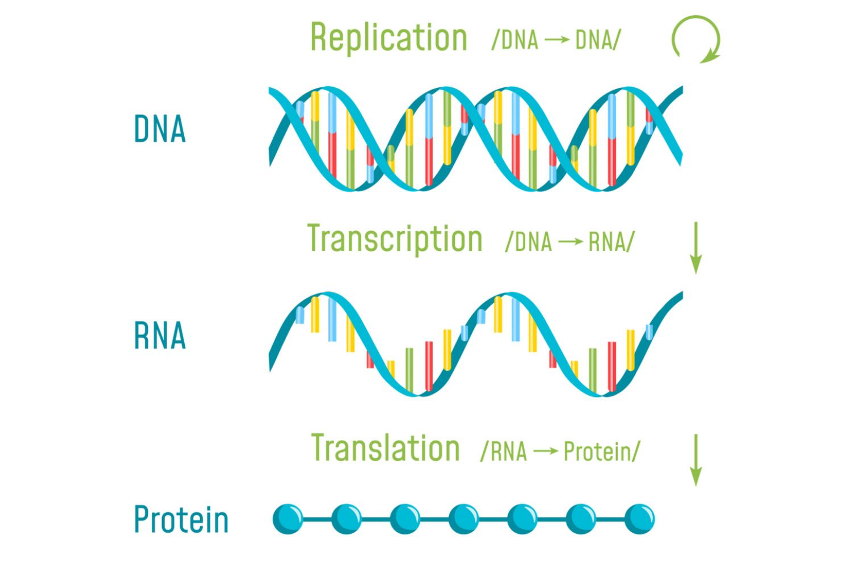
\includegraphics[width=0.5\linewidth]{\toplevelprefix/chapters/chapter1/figs/DNAs.png}
%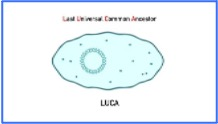
\includegraphics[width=0.28\linewidth]{\toplevelprefix/chapters/chapter1/figs/Luca.jpg}
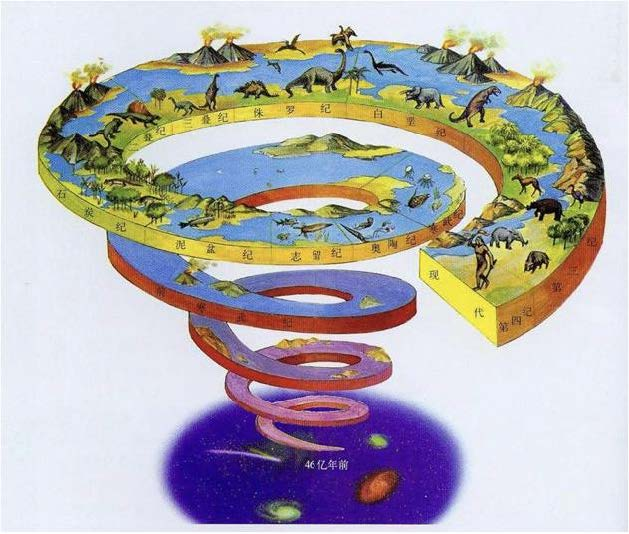
\includegraphics[width=0.40\linewidth]{\toplevelprefix/chapters/chapter1/figs/Evolution.jpg}
    \caption{种系发生智能的演化:关于外部世界的知识被编码并通过 DNA(左图)传递,然后从 DNA 解码为 RNA、蛋白质等。在生命演化的早期阶段(右图),智能通过(随机的)基因突变和自然选择——“适者生存”——在物种层面发展知识,这可以被视为一种原始的强化学习形式。}
    \label{fig:phylogenetic}
\end{figure}
\begin{figure}
    \centering
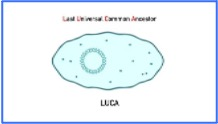
\includegraphics[height=0.19\linewidth]{\toplevelprefix/chapters/chapter1/figs/Luca.jpg}
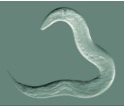
\includegraphics[height=0.19\linewidth]{\toplevelprefix/chapters/chapter1/figs/Worm.jpg}
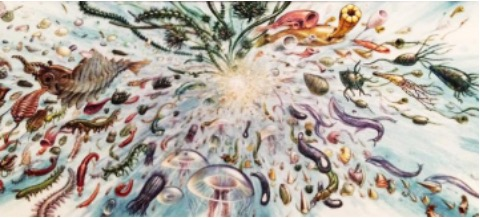
\includegraphics[height=0.19\linewidth]{\toplevelprefix/chapters/chapter1/figs/Cambrian.jpg}
    \caption{生命的演化:从生活在三十五亿至四十三亿年前、类似单细胞生物的现今所有生命的共同祖先(名为 LUCA——最后普遍共同祖先),到大约五亿五千万年前蠕虫状物种(中图)首次出现神经系统,再到大约五亿三千万年前寒武纪(右图)生命形式的大爆发。}
    \label{fig:evolution}
\end{figure}

{\em 个体发育智能}(The ontogenetic intelligence)指的是个体在其特定的生存环境中,通过自身的感官、记忆和预测进行学习,并据此改进和调整其行为的机制。个体发育学习是在大约五亿五千万到六亿年前神经系统(在蠕虫状生物中)出现之后才成为可能的,如 \ref{fig:evolution} 中图所示。也就是说,拥有了感觉和神经系统后,除了从 DNA 或基因中继承的知识外,个体还能够不断形成和完善自己关于世界的知识,这也被称为记忆。这种能力极大地增强了个体的生存机会,并促成了大约五亿三千万年前寒武纪生命形式的大爆发。与种系发生学习相比,个体发育学习的效率和可预测性都显著更高,个体在其生命周期内的有限资源下即可实现。

值得注意的是,这两种学习机制都依赖于某种形式的反馈(来自外部环境)来进行学习,即根据物种或个体的行为\footnote{物种的基因突变或个体的行为。}给予惩罚(死亡)或奖励(食物)。因此,所有智能生物,无论是作为物种还是作为个体,都依赖于一个闭环反馈机制来学习和增进其关于世界的知识。我们还注意到,从植物到鱼类,再到鸟类和哺乳动物,越是高等的物种,就越依赖其个体发育的学习能力。它们在出生后与父母待在一起、向父母学习的时间越来越长,因为同一物种的个体需要在极为多样的环境中生存。

\paragraph{人类智能的演化。}

自约31.5万年前智人出现以来,一种全新且更高形式的智能应运而生,其演化方式更为高效和经济。几千年前,语言得以发展,先是口头语言\footnote{人们曾认为梵语是第一种口头语言,其历史可追溯至公元前5000年。},后是书面语言\footnote{苏美尔语被认为是现存最古老的书面语言之一,最早于公元前3100年左右在美索不达米亚南部得到证实。}。参见图\ref{fig:human-intelligence}。语言使得个体之间能够交流并分享有用的信息。因此,一个人类社群或社会能像一个单一的智能有机体一样运作,其学习速度远超任何个体,拥有的知识也远胜任何个体。在某种程度上,书面语言或文本扮演着类似于DNA和基因的角色,它们使得人类社会能够积累关于世界的知识,并将其传承给后代。我们可以将这类智能称为{\em 社会智能},以区别于物种的系统发育智能和个体的个体发育智能。这种知识的积累方式,为古代文明奠定了基础。
\begin{figure}
    \centering
    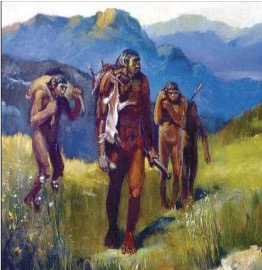
\includegraphics[height=0.25\linewidth]{\toplevelprefix/chapters/chapter1/figs/Spoken-language.jpg}
   \hspace{5mm} 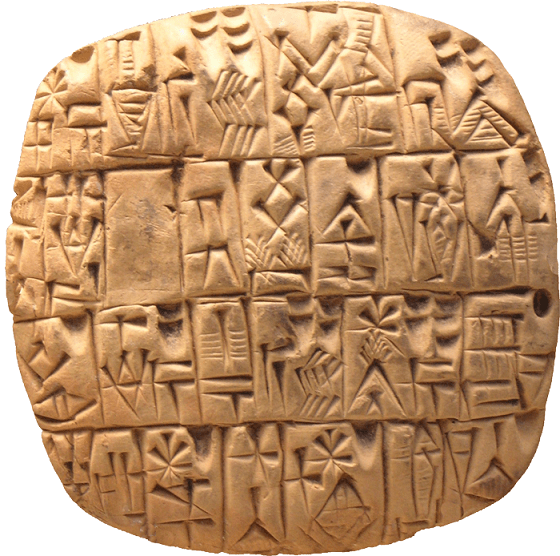
\includegraphics[height=0.25\linewidth]{\toplevelprefix/chapters/chapter1/figs/Cuneiform.png}
   \hspace{5mm} 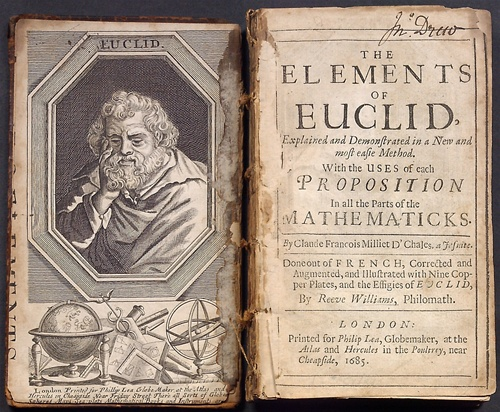
\includegraphics[height=0.25\linewidth]{\toplevelprefix/chapters/chapter1/figs/adopt-euclid1685-2.jpg}
    \caption{口头交流和口头语言(公元前10000年至5000年之间)、书面语言(约公元前3000年)以及数学(约公元前500年至300年)的发展,是人类智能演化史上的三个关键里程碑。}
    \label{fig:human-intelligence}
\end{figure}

奇迹般地,大约在几千年前,人类智能发生了另一次量子跃迁,使得哲学家和数学家能够发展出似乎远超经验知识范畴的知识。诸如数、空间和时间等抽象数学概念和符号,以及数理逻辑的发展,共同构成了一种服务于现代科学的全新而精确的语言。此外,人类还发展出了基于逻辑推演或科学实验来提出新假说并验证其正确性的能力。这使得人类首次能够超越被动的经验手段,主动地发展新知识。人们相信,进行这些高层次知识发展的能力为人类所独有。这种先进的智能形式被称为“人工智能”(AI),该术语由约翰·麦卡锡于1956年在达特茅斯夏季研讨会上提出。

因此,根据我们从自然界中所学到的,从今往后,每当我们使用“智能”一词时,都需要非常具体地指明其所处的层次与形式:
\begin{equation}
\mbox{\textbf{系统发育智能}} \;
   \Longrightarrow \; \mbox{\textbf{个体发育智能}} \; \Longrightarrow \; 
   \mbox{\textbf{社会智能}}
   \; \Longrightarrow \; 
   \mbox{\textbf{人工智能}}。
\end{equation}
做出清晰的刻画和区分是必要且重要的,因为我们希望将智能作为一个科学和数学的课题来研究。尽管不同层次/形式的智能或许都以学习关于世界的有用知识为共同目标,但其背后的具体计算机制和物理实现却极有可能不尽相同。我们相信,在读完本书后,读者将能更好地理解和领会这些差异。因此,我们将把关于通用智能的更多讨论留到最后一章(第\ref{ch:future}章)。


%在生物学领域,洛伦兹和廷贝亨是研究动物行为(尽管不是智能本身)的先驱。在认知科学领域,历史悠久,包括行为主义者(强化学习)、格式塔心理学家等。

%科学带来的启示。诺伯特·维纳的传记:《信息时代的黑暗英雄:寻找控制论之父诺伯特·维纳》(由康威和西格尔曼著)。与许多生物学家的联系。维纳在学生时代曾学习动物学。


\paragraph{机器智能的起源——控制论。}
20世纪40年代,部分出于战时的需要,自然界中的智能激发了当时的科学家们,他们试图用机器模仿动物的智能,这催生了由诺伯特·维纳所倡导的“控制论”运动。维纳在哈佛大学攻读本科学位时主修动物学,但后来成为了一名数学家和控制理论家。维纳毕生都热衷于理解和开发能够模仿动物智能行为的自主系统。如今,人们常常将控制论纲领狭隘地解读为主要关于反馈控制系统,而维纳确实在这一领域做出了他最重要的技术贡献。但控制论纲领的内涵远比这更为广博和深刻。它更关乎对智能整体\footnote{至少是在动物的层面上。}的理解,并切实影响了整整一代的著名科学家,包括沃伦·麦卡洛克、沃尔特·皮茨、克劳德·香农、约翰·冯·诺依曼和艾伦·图灵。

\begin{figure}
    \centering
    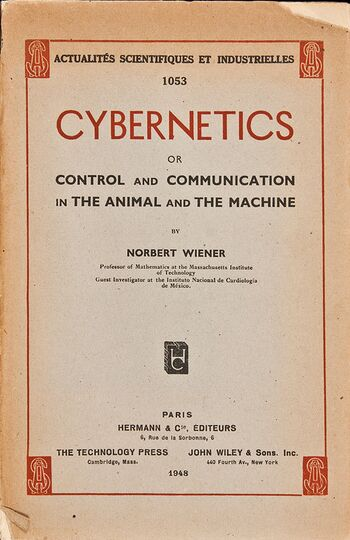
\includegraphics[height=0.4\linewidth]{\toplevelprefix/chapters/chapter1/figs/Cybernetics1.jpg}
    \hspace{10mm} 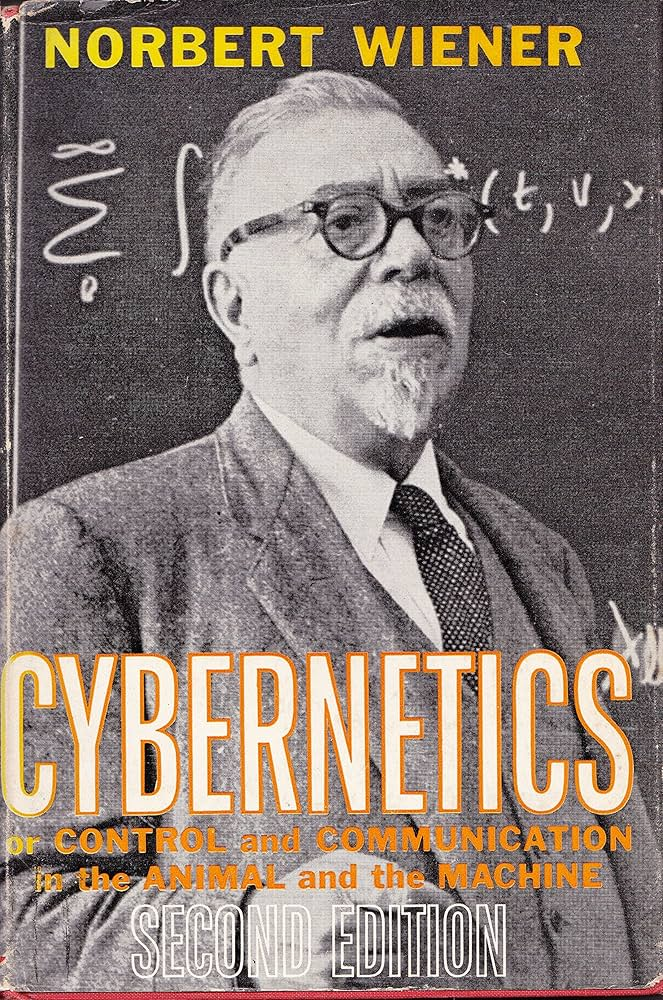
\includegraphics[height=0.4\linewidth]{\toplevelprefix/chapters/chapter1/figs/Cybernetics2.jpg}
    \caption{诺伯特·维纳的著作《控制论》,左图为1948年出版的第一版 \cite{Wiener-Cybernetics-1948},右图为1961年出版的第二版 \cite{Wiener-Cybernetics-1961}。}
    \label{fig:cybernetcis}
\end{figure}

维纳(Wiener)或许是第一位将智能作为{\em一个系统}来研究的学者,而不仅仅是关注其某个组成部分或某个方面。他在其1948年出版的著名著作{\em《控制论:或关于在动物和机器中控制和通信的科学》}\cite{Wiener-Cybernetics-1948}中,详尽阐述了他对智能的全面看法。在这本书及其1961年出版的第二版\cite{Wiener-Cybernetics-1961}(参见图\ref{fig:cybernetcis})中,他试图确定智能系统所必需的若干特性和机制,包括(但不限于):
\begin{itemize}
    \item 如何{\em测量和存储}信息(在大脑中)以及如何与他人通信。\footnote{诺伯特·维纳(Norbert Wiener)首次指出,“信息”既非物质也非能量,而是一个独立的研究量。} 这引导了克劳德·香农(Claude Shannon)在1948年创立信息论和编码理论。
    \item 如何基于现有信息来{\em纠正}预测和估计中的{\em错误}。诺伯特·维纳本人在20世纪40年代帮助建立了基于闭环反馈的控制系统理论。
    \item 如何在与潜在的非合作对手或对抗性环境的交互中,学会{\em做出更好的决策}。约翰·冯·诺依曼(John von Neumann)于1944年将其形式化为博弈论。
\end{itemize}
1943年,在维纳控制论思想的极大推动下,精神病学家沃伦·麦卡洛克(Warren McCulloch)和逻辑学家沃尔特·皮茨(Walter Pitts)共同建立了首个神经元的计算模型\cite{McCulloch-Pitts},称之为{\em人工神经元},其示意图见后文图\ref{fig:neuron}。基于此模型,在20世纪50年代,弗兰克·罗森布拉特(Frank Rosenblatt)构建了一台名为{\em Mark I 感知机}的物理机器,该机器由数百个此类人工神经元组成的网络构成。感知机是第一个被物理实现的人工神经网络,参见图\ref{fig:perceptron}。值得注意的是,约翰·冯·诺依曼于1945年提出的通用计算机体系结构,其设计目标也是为了促进构建能够物理实现控制论所提机制的{\em计算机器}。

敏锐的读者可能已经注意到,20世纪40年代确实是一个神奇的时代:许多奠基性的思想在那一时期诞生,众多影响深远的理论也在那时被建立,其中包括神经元的数学模型、人工神经网络、信息论、控制论、博弈论以及计算机器。图\ref{fig:god-fathers}展示了这些理论的一些先驱。众所周知,上述每一项工作都在其后的几十年中发展成为一个科学或工程领域的基础,并对我们产生了巨大影响。所有这些基础理论的诞生,都源于尝试开发能够模拟自然智能的机器这一目标的启发和驱动。根据历史记载,维纳的控制论运动几乎影响了所有这些学者及其工作。
\begin{figure}
    \centering
    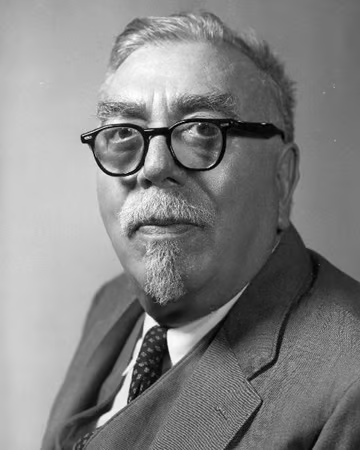
\includegraphics[height=0.3\linewidth]{\toplevelprefix/chapters/chapter1/figs/Wiener.png}
    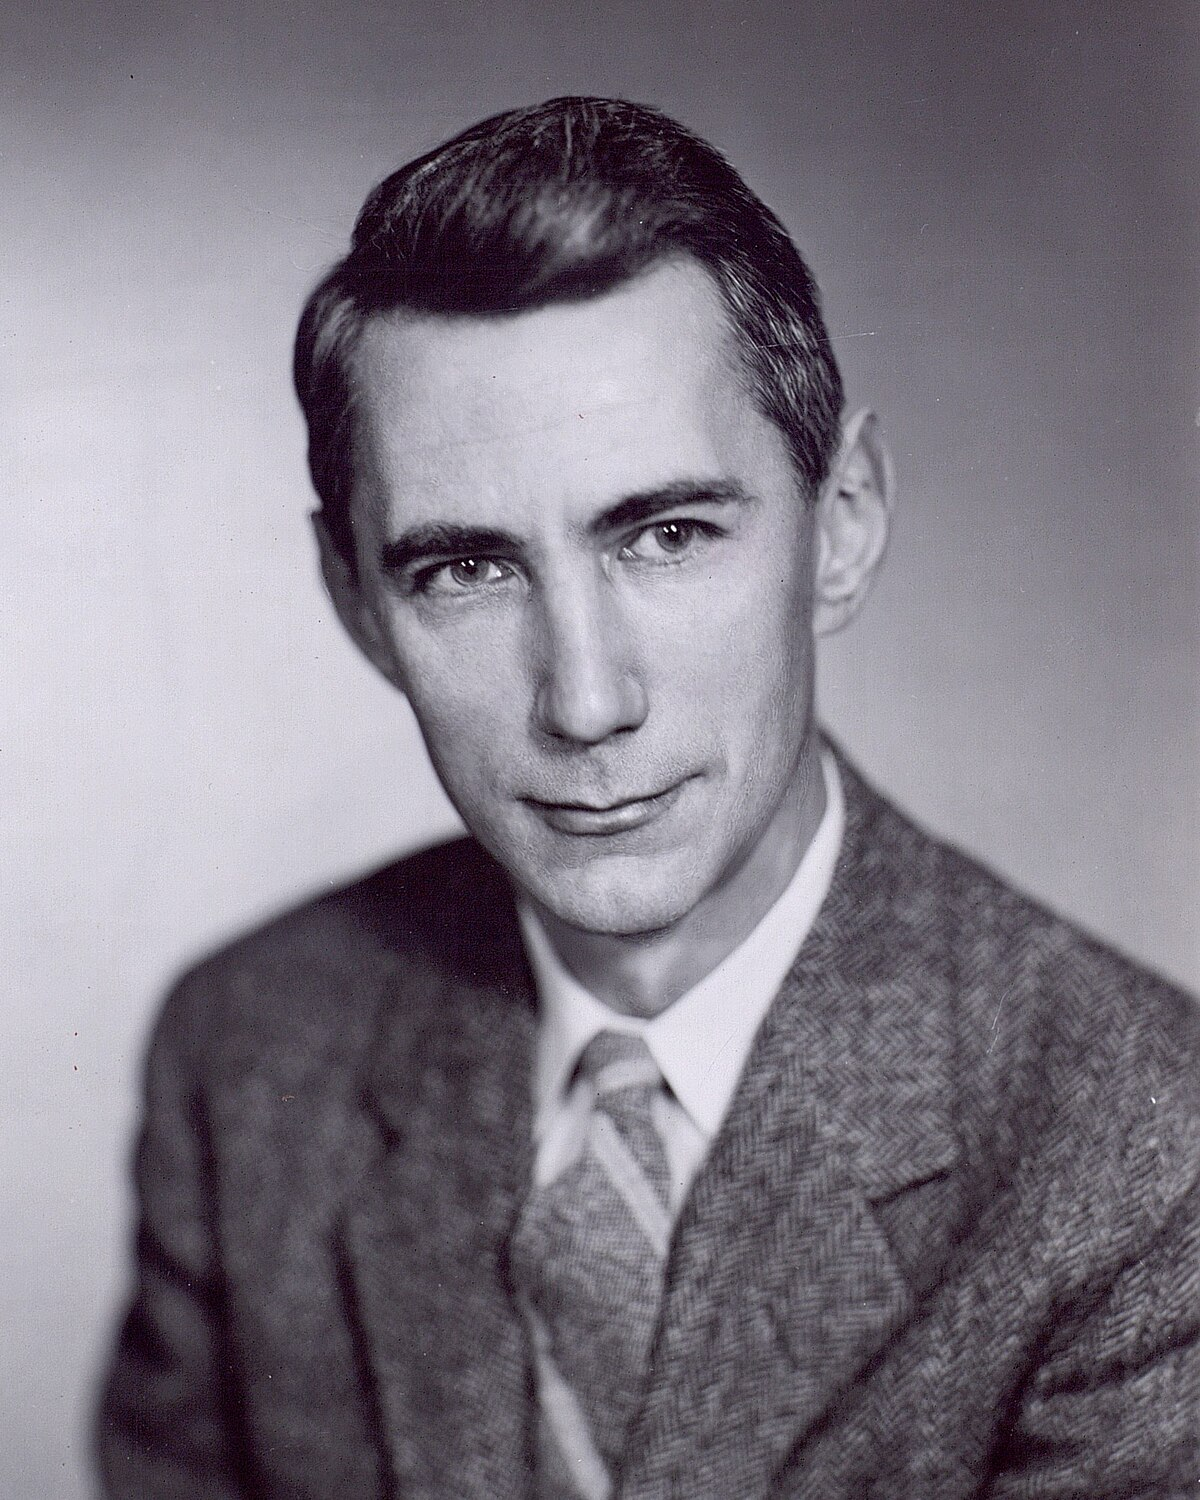
\includegraphics[height=0.3\linewidth]{\toplevelprefix/chapters/chapter1/figs/Shannon.jpg}
    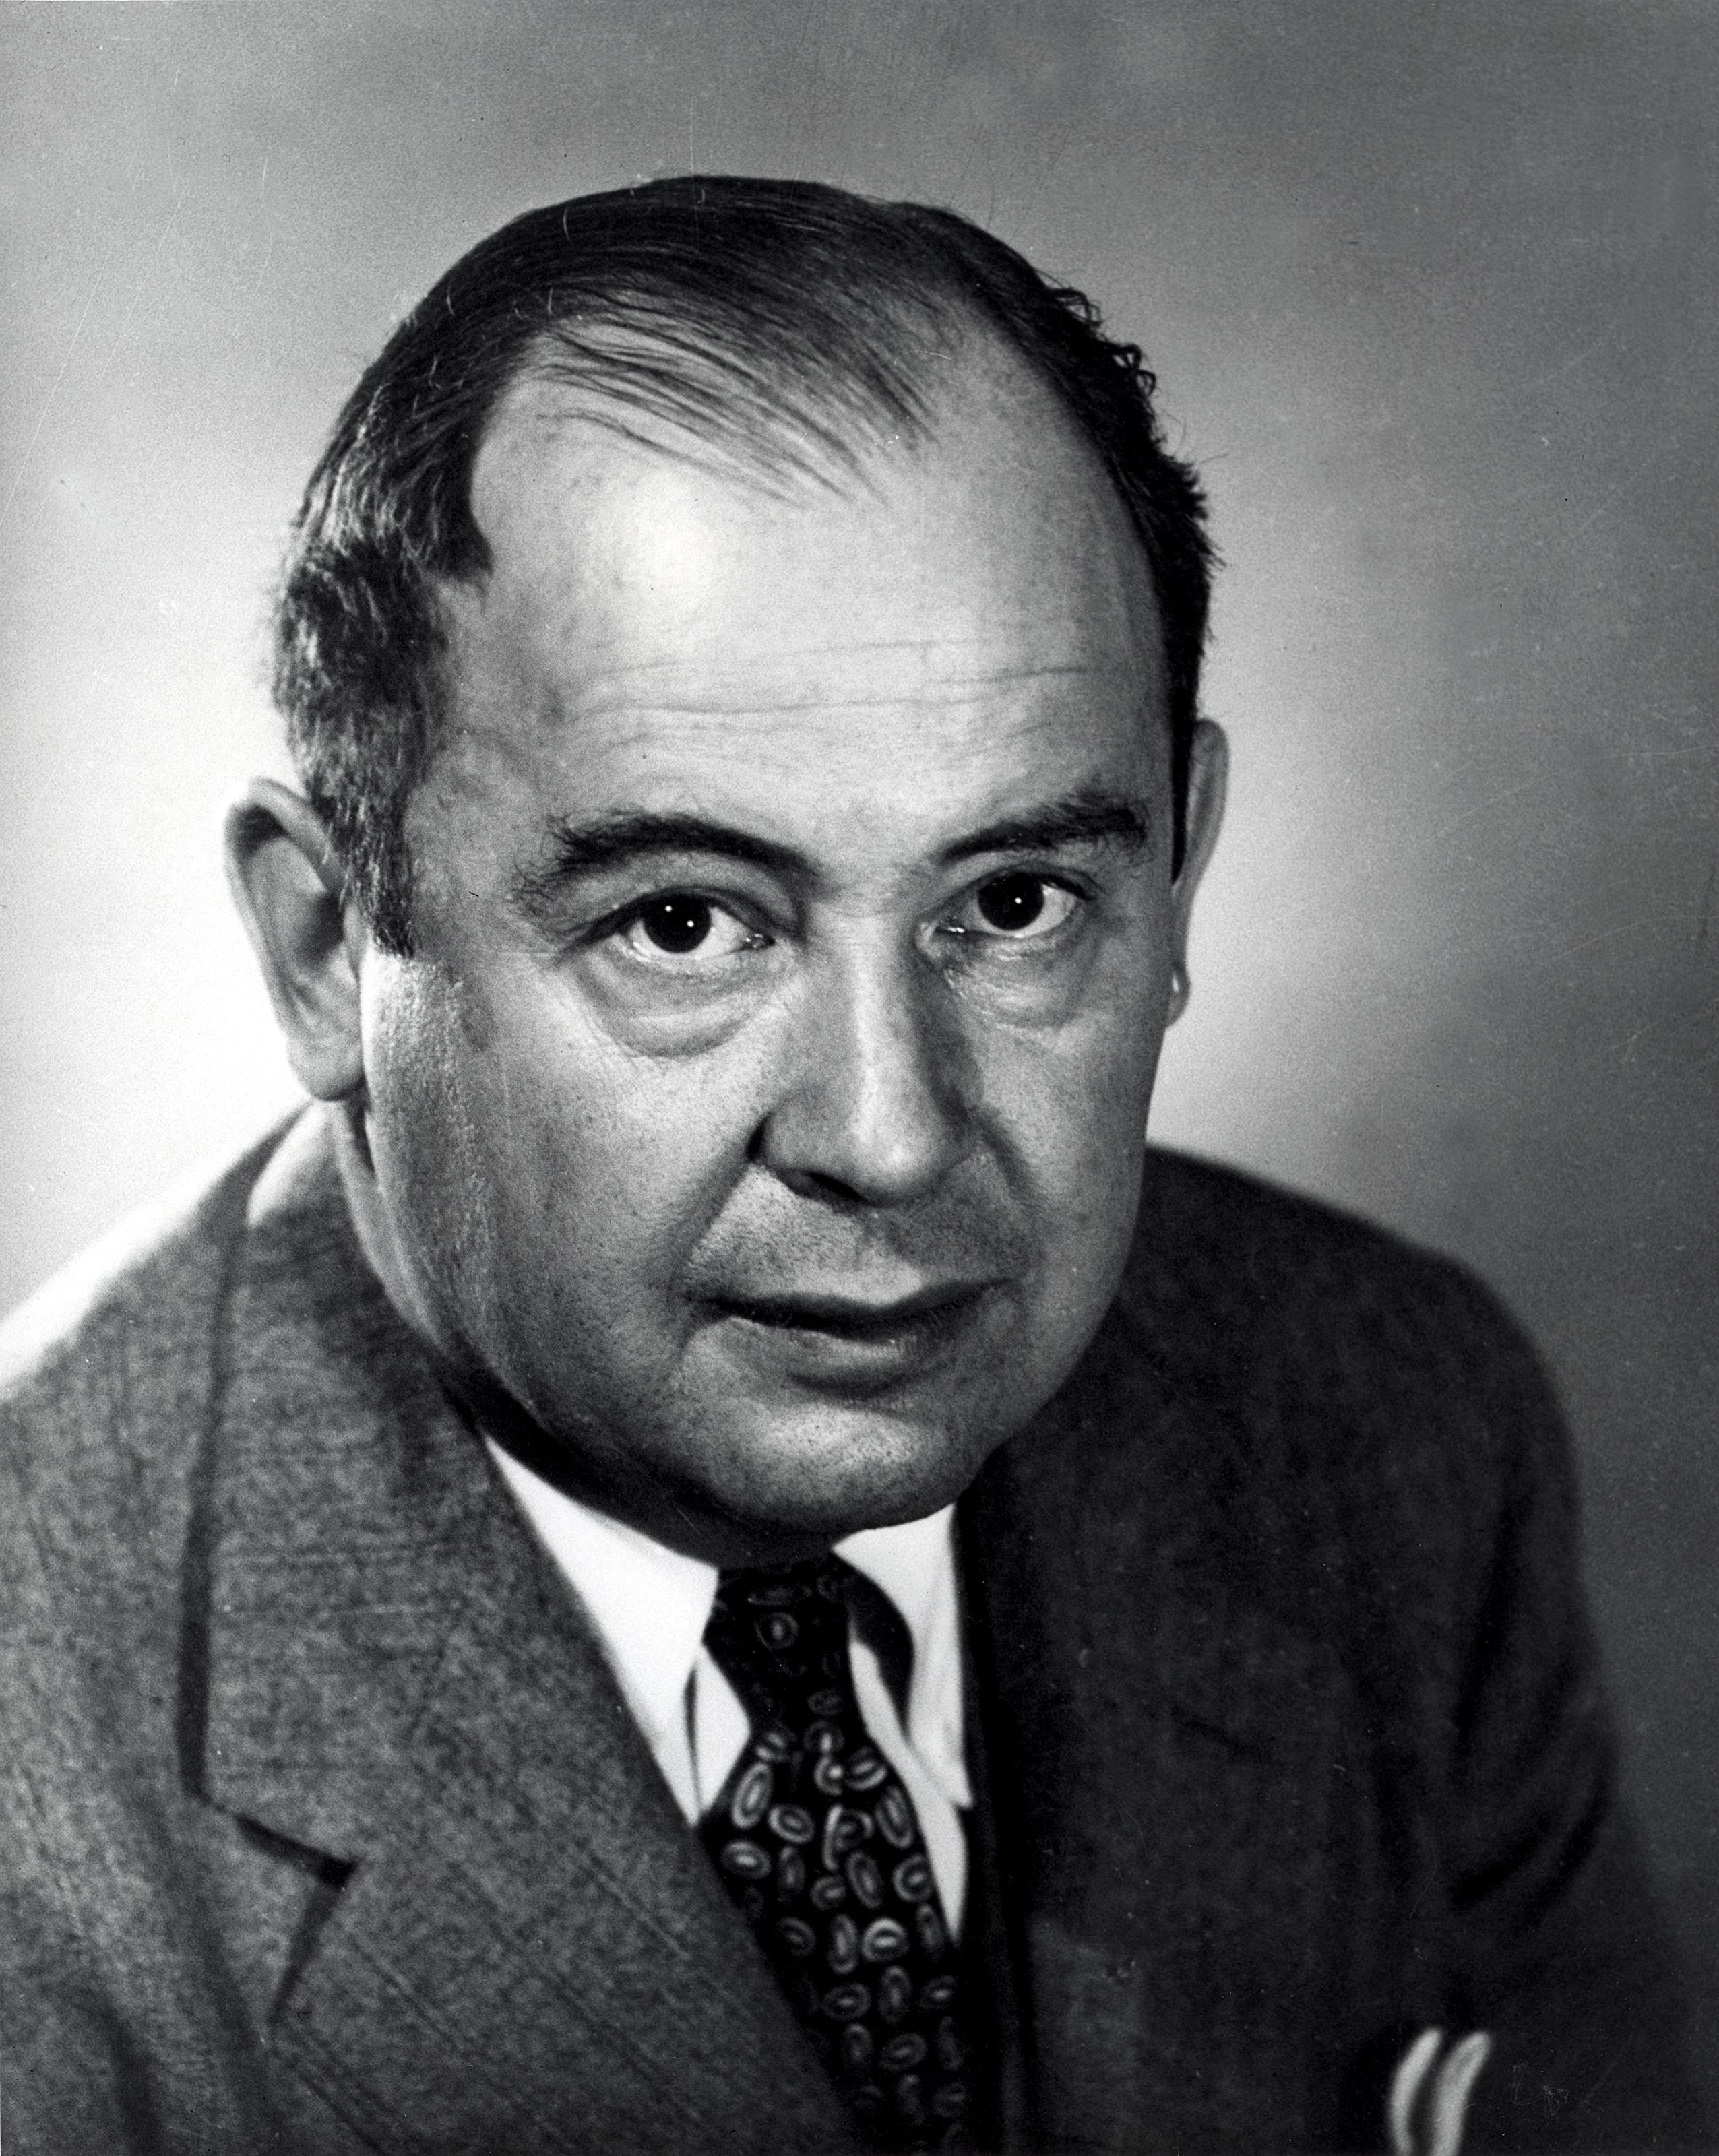
\includegraphics[height=0.3\linewidth]{\toplevelprefix/chapters/chapter1/figs/neumann.jpg}
    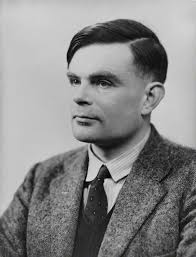
\includegraphics[height=0.3\linewidth]{\toplevelprefix/chapters/chapter1/figs/Turing.jpeg}
    \caption{为智能奠定理论与计算基础的先驱们:诺伯特·维纳(控制论与控制理论)、克劳德·香农(信息论)、约翰·冯·诺依曼(博弈论)以及艾伦·图灵(计算理论)。}
    \label{fig:god-fathers}
\end{figure}

尽管维纳在其著作中已经指出了智能的许多关键特征和机制,但没有迹象表明他知道如何将所有这些机制恰当地整合在一起,以构建一个完全自主的智能系统。以今天的知识来看,他关于这些机制的某些观点并不完全准确或完整。特别地,在《控制论》第二版的最后一章中 \cite{Wiener-Cybernetics-1961},他指出,若要设计一个机器学习系统来模拟自然界中典型的学习机制,{\em 处理非线性} 至关重要。但他并未对这一难题给出任何具体而有效的解决方案。不过,为他辩护的是,在当时,鲜有人知晓如何解决这个问题,因为就连处理线性模型和系统的理论也尚处于起步阶段。

尽管如此,我们仍不禁惊叹于维纳对非线性重要性的远见卓识。正如我们将在本书中看到的,答案直到最近才被发现:通过深度神经网络实现的渐进线性化和变换,可以有效地处理非线性问题(参见第 \ref{ch:representation} 章)。此外,我们还将在本书中尝试展示,如何将上文列出的所有这些机制自然地整合到一个完整的系统中,使其展现出自主智能系统的特征(参见第 \ref{ch:autoencoding} 章和第 \ref{ch:closed-loop} 章)。

\paragraph{人工智能的起源。}
从维纳的《控制论》一书的副标题——{\em “动物与机器的控制与通信”}——可以看出,20世纪40年代的研究主要旨在模拟动物层面的智能。正如我们之前提到的,20世纪40年代前后关于智能的研究议程,在很大程度上是由诺伯特·维纳的控制论运动所主导的。

艾伦·图灵是最早注意到这一局限性的人之一。在他1950年发表的著名论文《{\em 计算机器与智能}》\cite{Turing-1950}中,图灵正式提出了一个问题:机器能否模仿甚至达到人类水平的智能,以至于其智能能力与人类无法区分。这就是现在众所周知的{\em 图灵测试}。

1955年前后,一群年轻而雄心勃勃的科学家试图脱离当时占主导地位的控制论运动和研究议程,以期有机会开创自己的学术传承。他们决定接受图灵提出的模仿人类智能的挑战,并提议于1956年夏天在达特茅斯学院举办一个研讨会。他们在提案的一份声明中明确表达了其意图:
\begin{quote}
    ``{\em 此项研究将基于一个猜想展开,即学习的每一个方面或智能的任何其他特征,原则上都可以被精确地描述,从而可以用机器来模拟。我们将尝试探寻如何让机器使用语言、形成抽象和概念、解决目前只有人类才能解决的各种问题,并进行自我提升。}''
\end{quote}
从本质上讲,他们希望形式化并研究那些将人类与动物区分开来的更高层次的智能。他们所考虑的主题涵盖了抽象、符号方法、自然语言和演绎方法(包括因果推断、逻辑演绎等)。研讨会的组织者,时任达特茅斯学院数学系青年助理教授的约翰·麦卡锡,创造了如今闻名遐迩的术语——“人工智能”(Artificial Intelligence, AI),用以概括那些被认为是{\em 人类智能所独有}的特征或机制。

\paragraph{“人工智能”的复兴,还是“控制论”的复兴?}
读者或许已经知道,在过去十年左右的时间里,机器智能经历了爆炸性的发展,其主要驱动力是深度人工神经网络的实践应用,而这一浪潮则是由杰弗里·辛顿及其学生在2012年的工作所引发的 \cite{krizhevsky2012imagenet}。这个时代也被誉为人工智能(AI)的“复兴”。然而,就人们实际尝试解决的任务(识别、生成和预测)以及迄今为止开发和实现的技术(强化、模仿、编码、解码、去噪和压缩)而言,我们很大程度上只是在模拟早期生命和动物智能所共有的机制。即便如此,正如我们将在本书中阐明的,当前的“AI”模型和系统也并未正确实现这些层面智能所需的所有必要机制,而这些机制在20世纪40年代的控制论运动中就已为人所知。

因此,严格来说,过去十年机器智能的进步与1956年达特茅斯研讨会所规划的“人工智能”纲领并不十分契合。相反,迄今为止取得的主要成就,与诺伯特·维纳在20世纪40年代提出的经典“控制论”纲领的目标更为相关。称当今时代为“控制论的复兴”或许更为恰当。\footnote{近期兴起的所谓用于自主智能机器人的“具身智能”,与控制论纲领的目标有着更多的相似之处。} 只有当我们从科学和数学的视角,完全理解了我们真正完成了什么,我们才能真正知晓还有哪些工作尚待完成,以及应该朝哪个方向去探索智能的真正本质。这正是本书的主要目的之一。


\section{学什么?}
\label{sec:what-to-learn}
%注:智能的概念可以非常宽泛和笼统,但这往往使其变得模糊不清。在此,我们试图对其主要内涵给出一个更精确的描述。我们的定义或许会显著缩小其范围,但却使其更具可实现性、可验证性,甚至(通过可计算的方式)可度量性。



\subsection{可预测性}
\label{sec:predictability}
承载有用信息的数据以多种不同形式存在。在最自然的形式下,它们可以被建模为可预测和可计算的序列。可预测和可计算序列的概念及其性质是计算理论的核心,并在很大程度上促成了计算机的发明 \cite{Turing-1936}。20世纪60年代,雷·所罗门诺夫、安德雷·柯尔莫哥洛夫及其他许多学者研究了可预测序列在(归纳)推理中的作用 \cite{Kolmogorov1998OnTO},并将其作为克劳德·香农经典信息论 \cite{Shannon-1948} 的一种推广。为了理解可预测序列的概念,让我们先从一些具体的简单例子开始。
\paragraph{标量情形。}

最简单的可预测离散序列,可以说就是自然数序列:
\begin{equation}
   {S} =  1, 2, 3, 4, 5, 6, \ldots, n, n+1, \ldots
\end{equation}
在该序列中,后一项 $x_{n+1}$ 被定义为其前一项 $x_n$ 加 1:
\begin{equation}
x_{n+1} = x_n + 1.    
\end{equation}
我们可以将可预测性的概念推广至任意序列 $\{x_n\}_{n=1}^\infty$(其中 $ x_n \in \mathbb{R}$),若其后一项 $x_{n+1}$ 总能由其前一项 $x_n$ 计算得出:
\begin{equation}
    x_{n+1} = f(x_{n}), \quad x_n \in \mathbb{R}, \; n =  1, 2, 3, \ldots
\end{equation}
其中 $f(\cdot)$ 是一个{\em 可计算}的(标量)函数。\footnote{此处我们强调函数 $f(\cdot)$ 本身是可计算的,例如,它可以在计算机上作为一个程序来实现。} 请注意,此处我们强调函数 $f(\cdot)$ 必须是可计算的。有许多函数可以被定义,但却是不可计算的。阿兰·图灵在1936年的开创性工作 \cite{Turing-1936} 为可计算性给出了严格的定义。在实践中,我们通常会进一步假设 $f$ 是高效可计算的,并具有诸如连续、可微等良好性质。当我们对更精细的可计算性概念及其在机器学习和智能中的作用有了更深入的了解后,这些性质的必要性将变得更加清晰。

\paragraph{多变量情形。}
当然,序列中后一项的值也可以依赖于它的前两项。例如,著名的{\em 斐波那契序列}定义如下:
\begin{equation}
    {S} = 1, 1, 2, 3, 5, 8, 13, 21, 34, 55, \ldots
\end{equation}
我们不难发现:
\begin{equation}
    x_{n+2} = x_{n+1} + x_{n}, \quad  x_n \in \mathbb{R}, \;  n = 1, 2, 3, \ldots
\end{equation}
类似地,我们可以将此递归关系推广为
\begin{equation}
    x_{n+2} = f(x_{n+1}, x_{n}), \quad x_n \in \mathbb{R}, \;  n =  1, 2, 3, \ldots
\end{equation}
其中 $f(\cdot,\cdot)$ 是任意以两个变量为输入的可计算函数。我们可以进一步将可预测性的概念推广到这样一个序列:其后一项的值依赖于其前 $d$ 项:
\begin{equation}
    x_{n+d} = f(x_{n+d-1}, \ldots,  x_{n}), \quad  x_n \in \mathbb{R}, \; n =  1, 2, 3, \ldots
    \label{eqn:recursive-d}
\end{equation}
预测时所依赖的前项数量 $d$ 被称为递归预测的{\em 阶}。上述表达式 \eqref{eqn:recursive-d} 也被称为{\em (自)回归}。这样的序列也称为{\em 自回归}序列。如果函数 $f$ 是一个线性函数,我们称之为线性(自)回归。

\paragraph{向量情形。} 
为简化表示,我们可以定义一个向量 $\vx \in \mathbb{R}^d$ 来汇集序列中连续的 $d$ 个值
\begin{equation}
    \vx_n \doteq [x_{n+d-1}, \ldots,  x_{n}]^\top, \quad \vx_n \in \mathbb{R}^d, \; n = 1, 2, 3, \ldots
\end{equation}
利用该表示法,递归关系 \eqref{eqn:recursive-d} 便可以方便地写成
\begin{equation}
    \vx_{n+1} = g(\vx_{n}) \; \in \mathbb{R}^d, \quad n =  1, 2, 3, \ldots
    \label{eqn:recursive-v}
\end{equation}
其中函数 $g(\cdot)$ 由 \eqref{eqn:recursive-d} 中的函数 $f$ 唯一确定,并以一个 $d$ 维向量作为输入。在不同语境下,这样的向量有时被称为“状态”或“令牌”。注意,\eqref{eqn:recursive-d} 中的方程表示一个从 $\mathbb{R}^d$ 到 $\mathbb{R}$ 的映射,而此处的方程 $g$ 则是一个从 $\mathbb{R}^d$ 到 $\mathbb{R}^d$ 的映射。


\paragraph{受控预测。}
我们也可以定义一个可预测序列,其依赖于另一个可预测序列作为输入:
\begin{equation}
    \vx_{n+1} = f(\vx_{n}, \vu_n) \; \in \mathbb{R}^d, \quad n =  1, 2, 3, \ldots,
\label{eqn:recursive-control}
\end{equation}
其中,$\{\vu_n\}$($\vu_n \in \mathbb{R}^k$)是一个(可计算的)可预测序列。换言之,下一个向量 $\vx_{n+1} \in \mathbb{R}^d$ 同时依赖于 $\vx_n \in \mathbb{R}^d$ 和 $\vu_n \in \mathbb{R}^k$。在控制论的语境中,序列 $\{\vu_n\}$ 通常被称为“控制输入”,而 $\vx_n$ 则被称为系统 \eqref{eqn:recursive-control} 的“状态”或“输出”。一个经典的例子是线性动力系统:
\begin{equation}
    \vx_{n+1} = \boldsymbol{A}\vx_n + \boldsymbol{B}\vu_n, \quad \boldsymbol{A} \in \mathbb{R}^{d\times d}, \boldsymbol{B} \in \mathbb{R}^{d\times k},
    \label{eqn:lineary-system} 
\end{equation}
该系统在控制论中得到了广泛的研究 \cite{Cal:Des}。

在很多情况下,控制输入由状态 $\vx_n$ 自身的一个可计算函数给出,例如:
\begin{equation}
    \vu_n = h(\vx_n), \quad n =  1, 2, 3, \ldots 
\end{equation}
因此,序列 $\{\vx_n\}$ 可由两个可计算函数 $f$ 和 $h$ 复合而成:
\begin{equation}
    \vx_{n+1} = f\big(\vx_{n}, h(\vx_n)\big), \quad n =  1, 2, 3, \ldots
    \label{eqn:recursive-closed-loop}
\end{equation}
这样一来,序列 $\{\vx_n\}$ 再次成为一个自回归可预测序列。当输入 $\vu_n$ 依赖于输出 $\vx_n$ 时,我们称所得序列是由一个“闭环”系统 \eqref{eqn:recursive-closed-loop} 产生的。由于闭环系统不再依赖于任何外部输入,我们称这样的系统已经变为{\em 自治的}。它可以被看作是自回归的一个特例。例如,若我们在上述线性系统 \eqref{eqn:lineary-system} 中选择 $\vu_n = \boldsymbol{F}\vx_n$,则闭环系统变为:
\begin{equation}
        \vx_{n+1} = \boldsymbol{A}\vx_n + \boldsymbol{B}\vu_n = \boldsymbol{A}\vx_n + \boldsymbol{B}\boldsymbol{F}\vx_n = (\boldsymbol{A}+ \boldsymbol{B}\boldsymbol{F})\vx_n,
    \label{eqn:lineary-system-closed}
\end{equation}
这是一个线性自回归。

% \paragraph{近似预测。}
% 如果在上述方程 \eqref{eqn:recursive-control} 中,输入序列 $\vu_n$ 是不可预测的,情况会怎样?一种极端情况是其完全不可预测,例如:
% \begin{equation}
%     \vx_{n+1} = f(\vx_{n}, \boldsymbol{\epsilon}_n), \quad n =  1, 2, 3, \ldots
%     \label{eqn:recursive-noise}
% \end{equation}
% 其中 $\boldsymbol{\epsilon}_n \in \mathbb{R}^k$ 为某种随机(高斯)噪声。在这种情况下,我们称如此定义的序列 $\{\vx_n\}$ 是“随机的”。显然,这样的序列不再是完全可预测的,至少在上述的确定性意义上不再是。

% 当噪声的幅度 $\|\boldsymbol{\epsilon}_n\|$ 很小,且函数 $f$ 对噪声的放大作用不显著时,我们有
% \begin{equation}
%     \vx_{n+1} \approx f(\vx_{n}, \boldsymbol{0}) + \nabla_{\boldsymbol{\epsilon}}f(\vx_{n}, \boldsymbol{0})   \boldsymbol{\epsilon}_n, \quad n =  1, 2, 3, \ldots
%     \label{eqn:recursive-noise-small}
% \end{equation}
% 其中第二项 $\|\nabla_{\boldsymbol{\epsilon}}f(\vx_{n}, \boldsymbol{0})   \boldsymbol{\epsilon}_n\|$ 的幅度很小。因此,$ \vx_{n+1}$ 主要由第一个确定性项决定,且其期望是可预测的:
% \begin{equation}
%     \mathbb{E}[\vx_{n+1}] \approx f(\vx_{n}, \boldsymbol{0}).
% \end{equation}
% 在这种情况下,我们称由 \eqref{eqn:recursive-noise-small} 定义的序列 $\{\vx_n\}$ 是“近似可预测的”。在实践中,我们经常在真实世界的数据中处理这类近似可预测性,因为测量噪声在这些数据中普遍存在。注意,取期望在本质上消除了随机噪声的影响,并使期望序列 $\{\mathbb{E}[\vx_n]\}$ 成为一个可预测序列。这样的过程通常被称为“去噪”。\DP{此处的“去噪”与第二/三章中的“去噪”之间的联系乍一看并不明显。例如,此处的去噪是针对自回归序列的,而后面的去噪是针对单个观测值的。这也与滤波不是一回事。我不太明白为什么需要这一段(至少是在这里)。}

\paragraph{连续过程。}
可预测序列在连续情形下有其自然的对应物。我们可以称之为可预测过程。与自然数序列类似,最简单的可预测连续过程是时间本身 $x=t$。

更一般地,我们称一个以 $\vx(t)$ 表示的过程是可预测的,如果在任意时刻 $t$,该过程在 $t+\delta t$ 时刻的值(其中 $\delta t$ 是一个无穷小增量)由其在 $t$ 时刻的值所决定。通常,值的变化量 $\delta \vx(t)$ 是连续且光滑的。因此 $\delta \vx(t) = \vx(t + \delta t) - \vx(t)$ 是无穷小的。可预测过程通常由(多元)微分方程描述:
\begin{equation}
    \dot{\vx}(t) = f(\vx(t)), \quad \vx \in \mathbb{R}^d. 
    \label{eqn:process}
\end{equation}

在系统理论的框架下 \cite{Cal:Des,Sastry-Nonlinear},上述方程也被称为状态空间模型。与离散情形类似,一个受控过程可由下式给出:
\begin{equation}
    \dot{\vx}(t) = f(\vx(t), \vu(t) ), \quad \vx \in \mathbb{R}^d, \vu \in \mathbb{R}^k,
    \label{eqn:process-controlled}
\end{equation}
其中 $\vu(t)$ 是一个可计算的输入过程。

\begin{example}
    例如,在物理学中,牛顿第二运动定律描述了如何在一个力 $\boldsymbol{F}(t) \in \mathbb{R}^3$ 的作用下,预测一个运动物体的轨迹 $\boldsymbol{x}(t) \in \mathbb{R}^3$:
\begin{equation}
    m\ddot{\boldsymbol{x}}(t) = \boldsymbol{F}(t).
\end{equation}
    当没有力作用,即 $\boldsymbol{F}(t) \equiv 0$ 时,上述定律简化为一个特例,即牛顿第一运动定律:物体将保持匀速直线运动:
\begin{equation}
   \ddot{\boldsymbol{x}}(t) = \boldsymbol{0} \; \Leftrightarrow \; \dot{\boldsymbol{x}}(t) = \boldsymbol{v}
\end{equation}
    其中 $\boldsymbol{v} \in \mathbb{R}^3$ 为某个恒定的速度矢量。
\end{example}




\subsection{低维性}\label{sec:intro-low-dimensionality}
\paragraph{学习预测。}
现在,假设你观测到或被给予了许多序列片段:
\begin{equation}
    \{S_1, S_2, \ldots, S_i, \ldots, S_N\}
\end{equation}
它们都来自某个可预测序列 $\{x_n\}_{n=1}^\infty$。不失一般性地,我们可以假设每个片段的长度为 $D \gg d$。因此,每个片段的形式为:
\begin{equation}
    S_i = [x_{j(i)}, x_{j(i)+1}, \ldots, x_{j(i)+D-1}]^\top \in \mathbb{R}^D
\end{equation}
其中 $j \in \mathbb{N}$。然后,给定一个新的片段 $S_t$,你需要预测其未来的值。

此处的一个难点在于,你通常不知道生成该序列的函数 $f$ 和阶数 $d$:
\begin{equation}
    x_{n+d} = f(x_{n+d-1}, \ldots,  x_{n}).
\label{eqn:sequence-order-d}
\end{equation}
因此,我们希望能以某种方式从给定的样本片段 $S_1, S_2, \ldots, S_N$ 中“学习”出 $f$ 和 $d$。因此,学习预测的核心任务是:
\begin{center}
{\em 给定一个可预测序列的许多采样片段,如何有效且高效地辨识出函数 $f$。}
\end{center}

\paragraph{可预测性与低维性。}
为确定预测函数 $f$,我们可以注意到任何可预测序列(例如由 \eqref{eqn:sequence-order-d} 给出)的片段所具有的一个共同特征。如果我们从该序列中取一个长片段(比如说,其长度满足 $D \gg d$),并将其视为一个向量:
\begin{equation}
    \vx_i = [x_i, x_{i+1}, \ldots x_{i+D-1}]^\top \in \mathbb{R}^D.
\end{equation}
那么,所有这些向量组成的集合 $\{\vx_i\}$ 远非随机,因此不可能占据整个 $\R^D$ 空间。相反,它们本质上至多有 $d$ 个自由度——即一旦给定任一向量 $\vx_i$ 的前 $d$ 个元素,其余元素的值便被唯一确定。换言之,所有的向量 $\{\vx_i\}$ 都位于一个 $d$ 维曲面上。在数学中,这样的曲面通常被称为子流形,记作 $\mathcal{S} \subset \R^D$。

\begin{figure}[t]
\centering
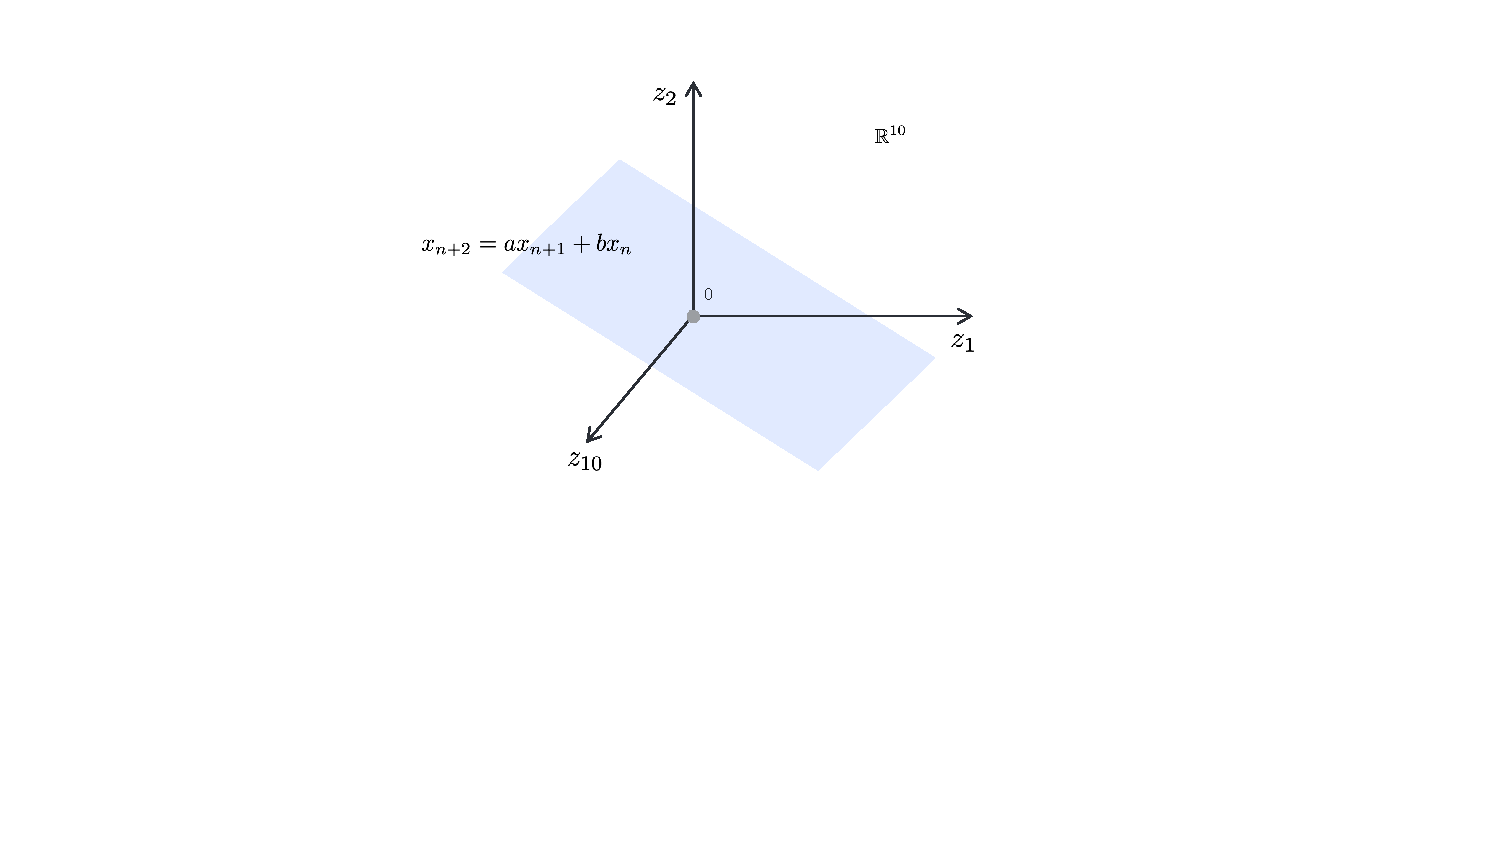
\includegraphics[width=0.6\linewidth]{\toplevelprefix/chapters/chapter1/figs/two-dimensional plane in R10.pdf}
    \caption{一个十维环境空间中的二维子空间。}
    \label{fig:lowdimplane}
\end{figure}
在实践中,如果我们选择的片段长度 $D$ 足够大,那么从同一预测函数中采样的所有片段都会位于一个内蕴维数为 $d$ 的曲面上,该维度远低于环境空间维度 $D$。例如,如果序列由如下的线性自回归模型给出:
\begin{equation}
    x_{n+2} = a\cdot x_{n+1} + b\cdot x_n,
    \label{eqn:sequence-2d}
\end{equation}
其中 $a, b \in \R$ 为常数。如果我们从这样的序列中采样长度为 $D =10$ 的片段,那么所有的样本点都将位于 $\R^{10}$ 空间中的一个二维平面或子空间上,如图 \ref{fig:lowdimplane} 所示。如果我们能够确定这个二维子空间,那么公式 \eqref{eqn:sequence-2d} 中的常数 $a$ 和 $b$ 就能被完全确定。

显而易见,如果预测函数 $f$ 是线性的,例如在 \eqref{eqn:lineary-system} 和 \eqref{eqn:lineary-system-closed} 给出的线性系统中,那么长片段总是位于某个低维线性子空间上。确定该预测函数在很大程度上等价于确定这个低维子空间,这个问题通常被称为主成分分析。我们将在第 \ref{ch:classic} 章中讨论这类经典模型和方法。

事实证明,这对于一般的可预测序列也基本成立:如果能确定所有片段样本所在的低维曲面,那么就能确定相关的预测函数 $f$。\footnote{在温和的条件下,低维曲面与函数 $f$ 之间存在一一映射关系。这一事实已被应用于诸如系统辨识等问题中,我们将在后面讨论这些问题。}对于可预测序列的片段所具有的这一特性,其重要性再怎么强调也不为过:{\em 一个可预测序列的所有长片段样本都位于一个低维子流形上。}正如我们将在本书中看到的,所有的现代学习方法,无论是隐式地还是显式地,本质上都在利用这一特性。%\yima{为曲面或子流形添加一幅插图。}

在现实世界的场景中,我们观测到的数据通常并非来自单个可预测序列。典型地,它们包含对多个可预测序列的观测。例如,一个视频序列可能包含多个运动物体。显而易见,在这种情况下,数据位于多个低维线性子空间或非线性子流形的混合体上,如\Cref{fig:mixture-models}所示。
\begin{figure}
    \centering
    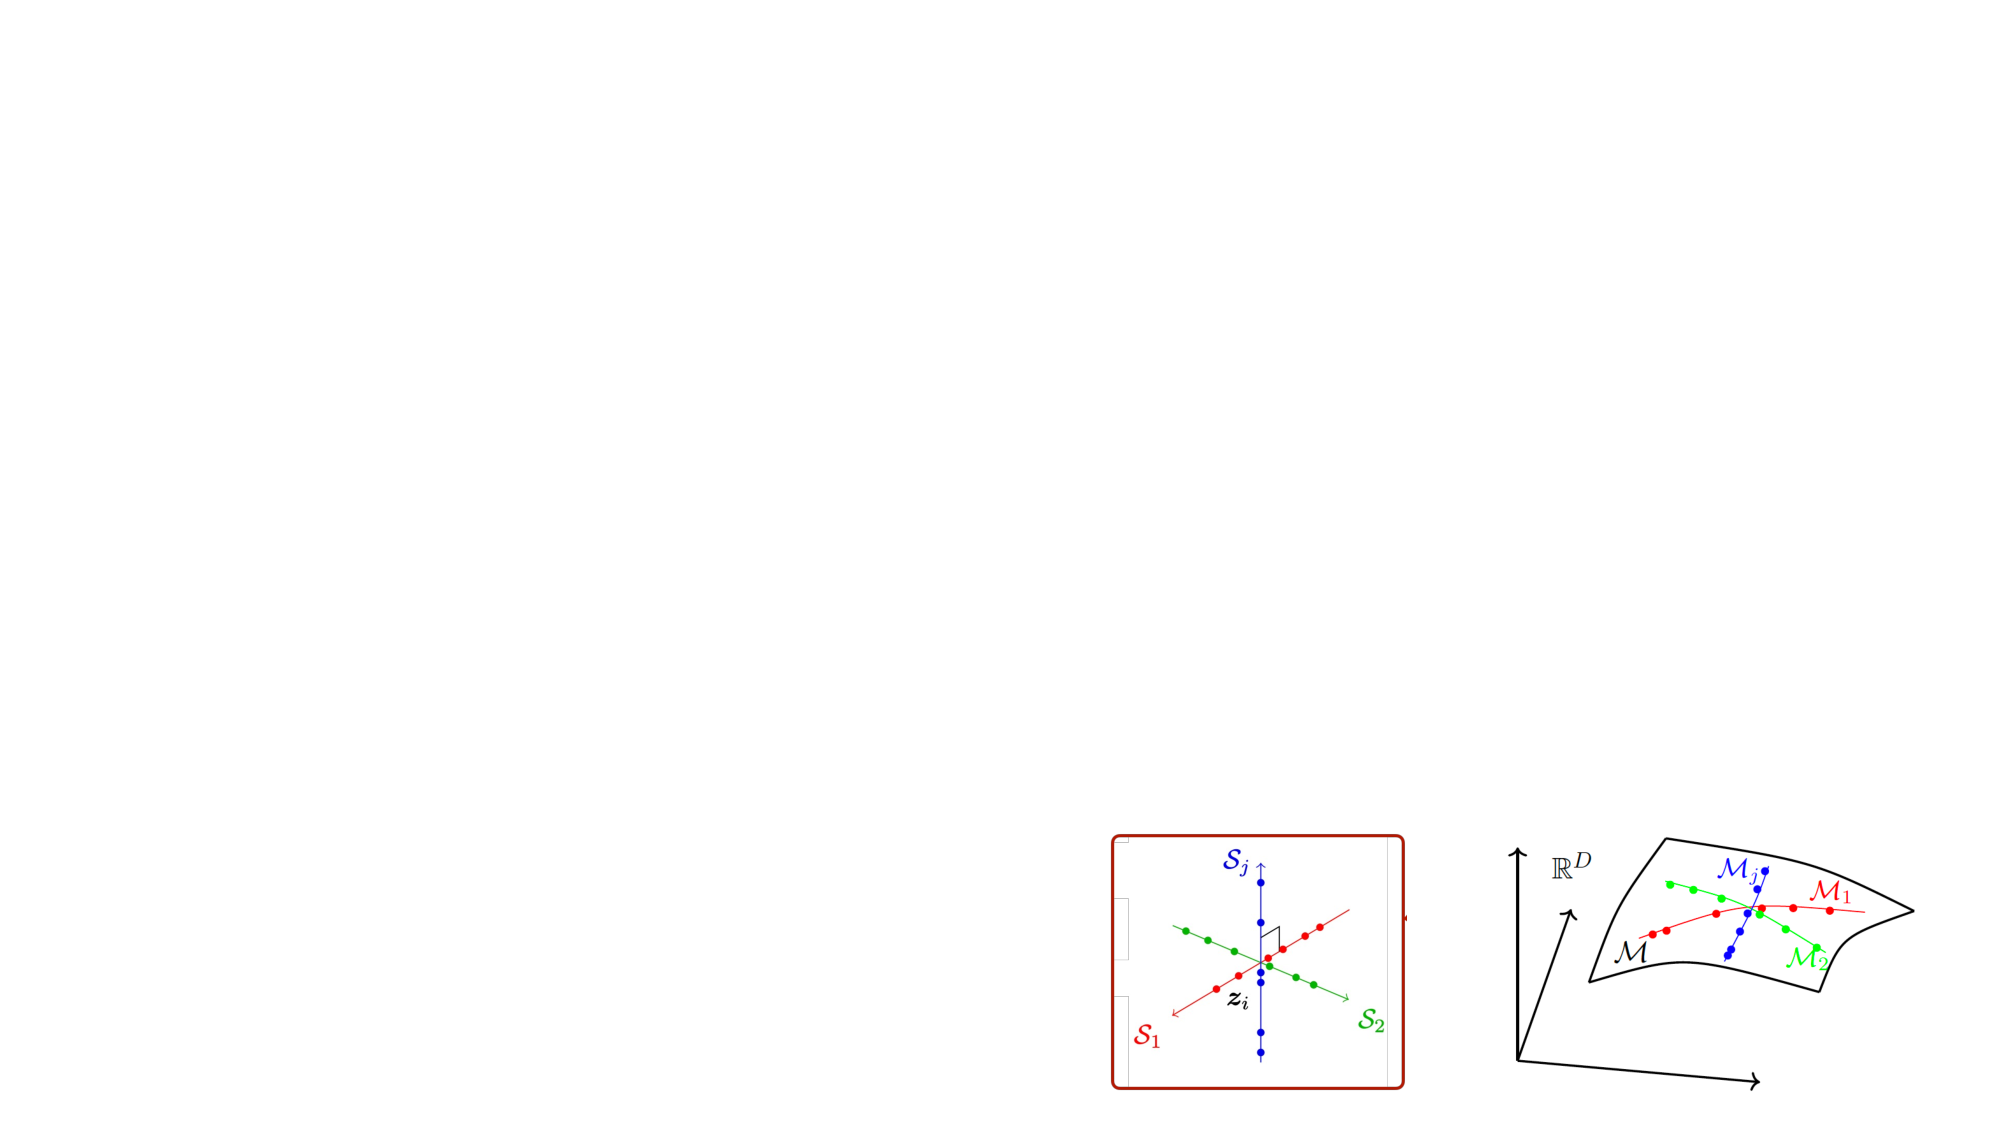
\includegraphics[width=0.8\linewidth]{\toplevelprefix/chapters/chapter1/figs/mixture.pdf}
    \caption{数据分布在(正交)子空间(左图)或子流形(右图)的混合体上。}
    \label{fig:mixture-models}
\end{figure}

\paragraph{低维度的性质。}
当然,可预测序列中的时间相关性并非数据呈低维的唯一原因。例如,所有图像构成的空间极其庞大,但其中大部分空间是由类似于\Cref{fig:noise-image}左图所示的无结构随机图像组成。然而,自然图像和视频是高度冗余的,因为其所有像素值之间存在很强的空间和时间相关性。正因如此,我们能轻易分辨一幅图像是带噪的还是干净的,如\Cref{fig:noise-image}中图和右图所示。因此,自然图像的分布具有非常低的内在维度(相对于图像的总像素数而言)。

\begin{figure}
    \centering
    
\includegraphics[height=0.30\linewidth]{\toplevelprefix/chapters/chapter1/figs/Gaussian-noise.png}\hspace{2mm} 
    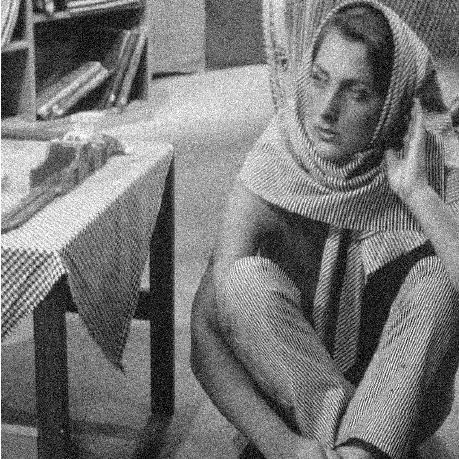
\includegraphics[height=0.30\linewidth]{\toplevelprefix/chapters/chapter1/figs/Standard-test-image-Barbara-of-size-512-512-pixels-including-Gaussian-noise-with.png} \hspace{2mm} 
    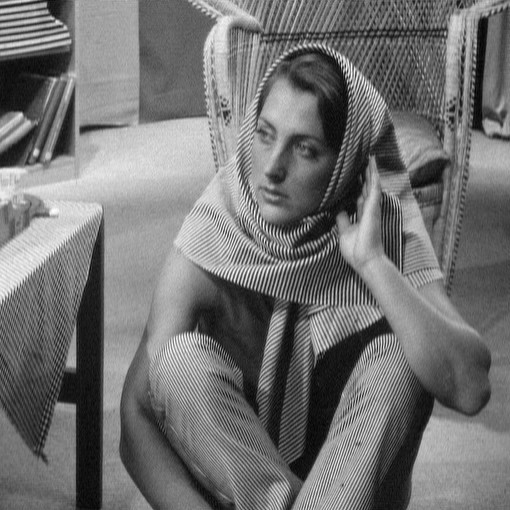
\includegraphics[height=0.30\linewidth]{\toplevelprefix/chapters/chapter1/figs/barbara.jpg}
    \caption{随机噪声图像、带噪图像与原始干净图像的对比。%\sdb{probably want to avoid using Lena given all the IEEE/PAMI-TC/etc.\ recent motions}
    }
    \label{fig:noise-image}
\end{figure}

鉴于学习低维结构这一任务的重要性和普遍性,《高维数据分析与低维模型:原理、计算与应用》({\em ``High-Dimensional Data Analysis with Low-Dimensional Models: Principles, Computation, and Applications''})\cite{Wright-Ma-2022}一书开篇便指出:``{\em 在高维空间中识别信号或数据的低维结构,是贯穿系统论、信号处理、模式识别、机器学习和统计学等众多工程与数学领域悠久历史的最基本问题之一。}''

请注意,通过将观测数据点$\vx$约束在低维曲面上,我们实际上使得$\vx$的各个分量彼此高度依赖,在某种意义上,也使得这些分量可以根据其他分量的值进行“预测”。例如,如果我们知道数据被约束在$\R^d$空间中的一个$d$维曲面上,那么除了预测之外,我们还可以对数据进行许多有用的操作:%\yima{Maybe some illustrations for these properties.}
\begin{itemize}
    \item \textbf{补全}:通常情况下,对于一个典型样本$\vx$,只要给定其超过$d$个分量,其余分量通常可以被{\em 唯一}确定。\footnote{预测成为该性质的一个特例。}
    \item \textbf{去噪}:假设一个样本$\vx$的各分量受到了{\em 小}噪声的扰动,通过将$\vx$投影回该曲面,可以有效地去除这些噪声。
    \item \textbf{纠错}:假设$\vx$中少数{\em 未知}分量被任意损坏,它们可以被有效且高效地纠正。
\end{itemize}
图\ref{fig:low-dim-properties}用一个低维线性结构——二维平面上的一维直线——阐释了这些性质。

\begin{figure}
    \centering
    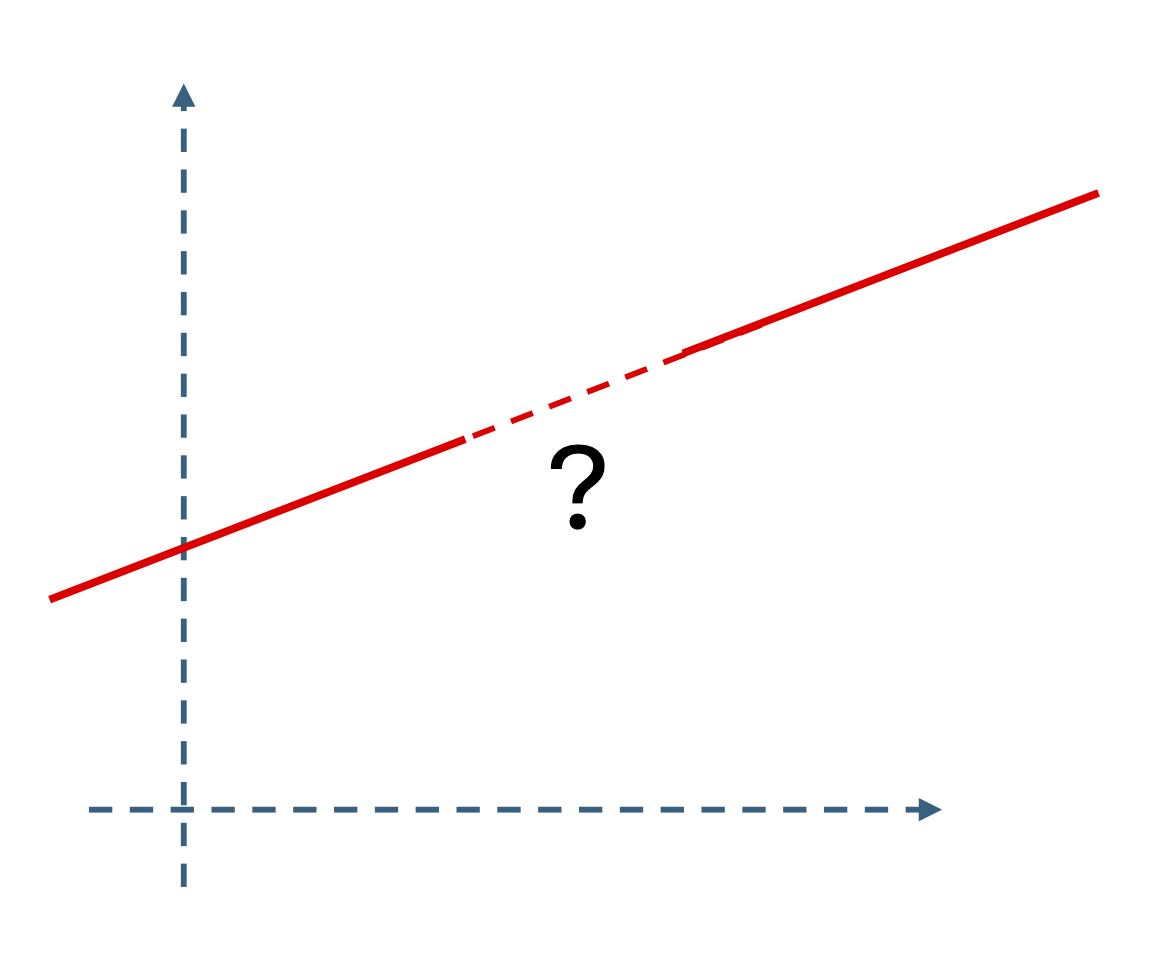
\includegraphics[height=0.28\linewidth]{\toplevelprefix/chapters/chapter1/figs/Completion-low-dim.png}     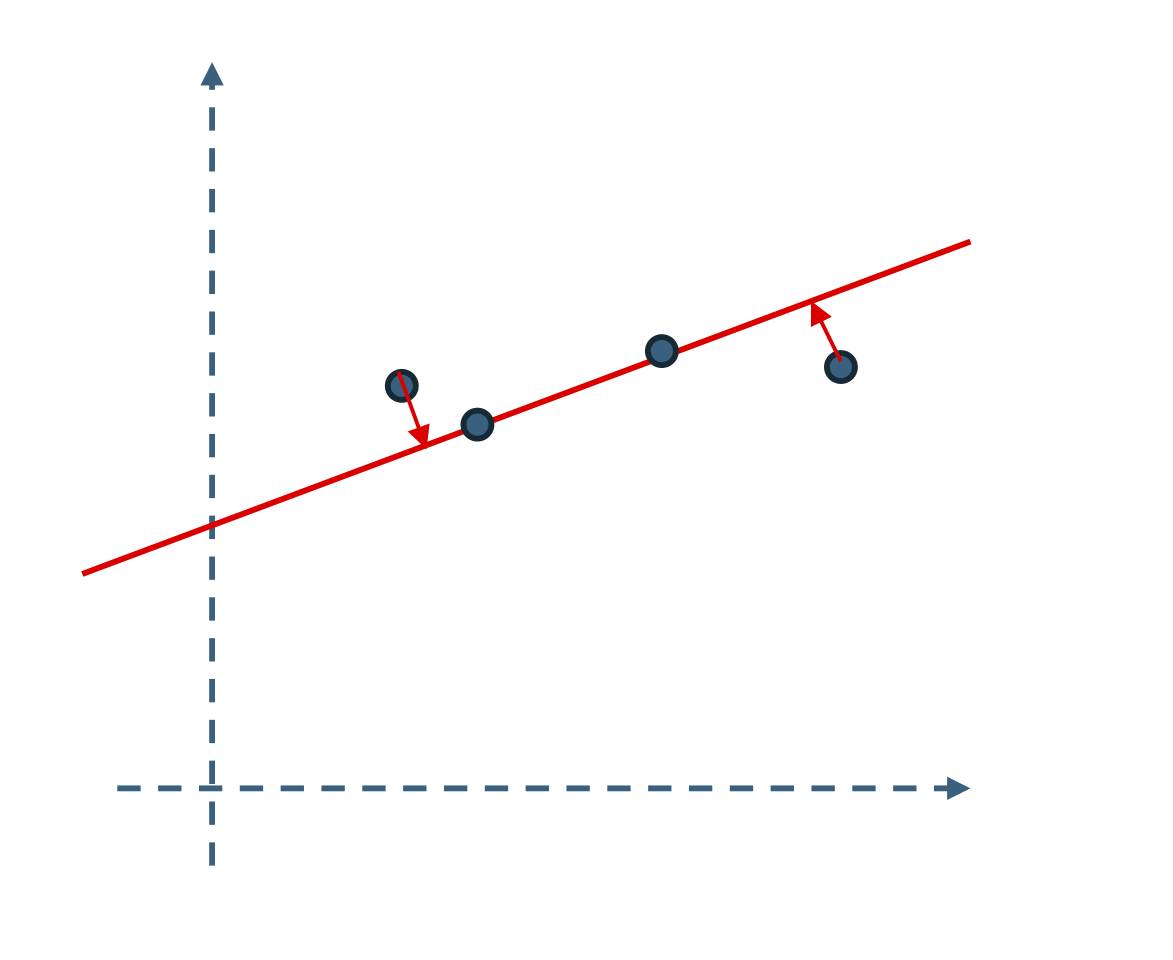
\includegraphics[height=0.28\linewidth]{\toplevelprefix/chapters/chapter1/figs/Denoising-low-dim.png} 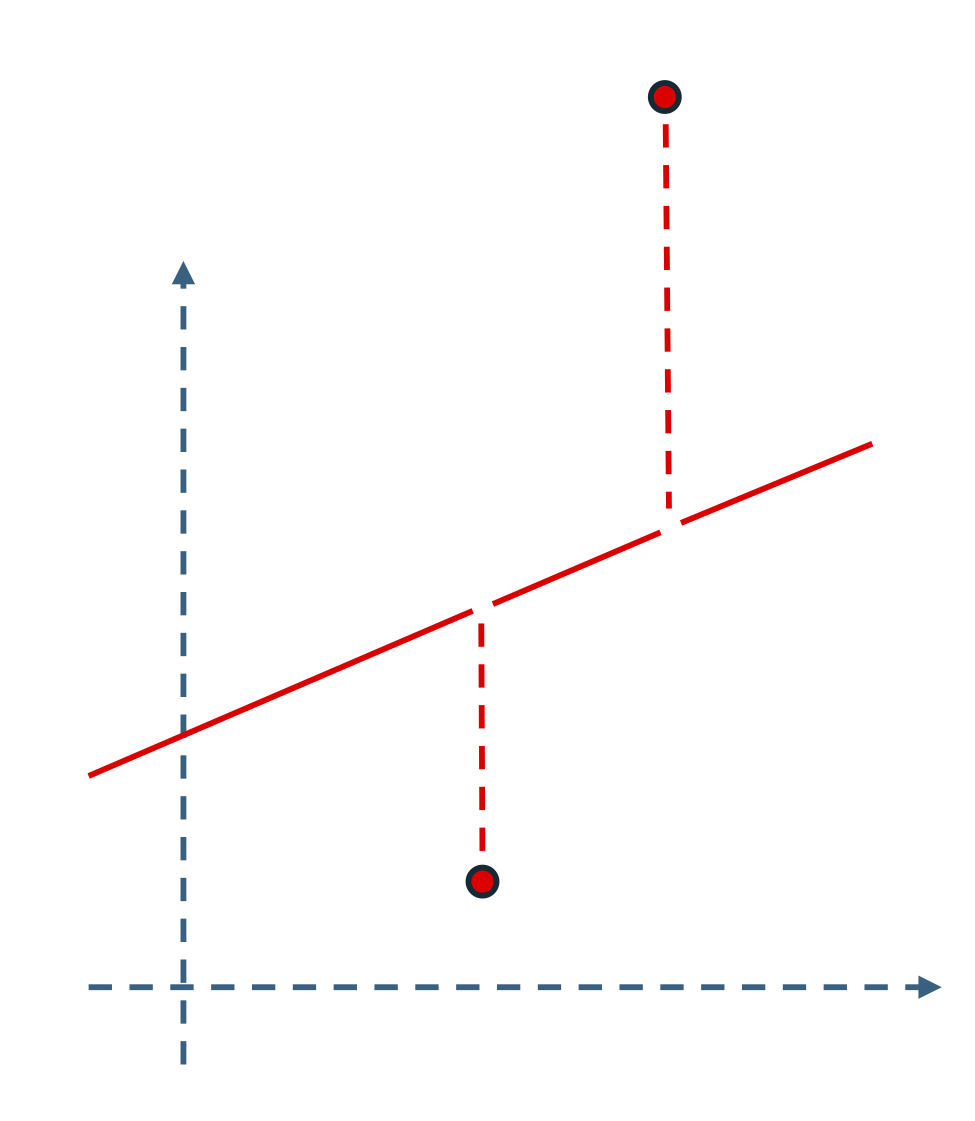
\includegraphics[height=0.32\linewidth]{\toplevelprefix/chapters/chapter1/figs/Correction-low-dim.png} 
    \caption{低维(线性)结构的性质图示:它支持补全(左)、去噪(中)和纠错(右)。}
    \label{fig:low-dim-properties}
\end{figure}

事实上,在温和的条件下,上述性质可以推广到高维空间中的许多其他低维结构\cite{Wright-Ma-2022}。有趣的是,正如我们将在本书中看到的,这些有用的性质,如补全和去噪,将启发我们找到学习此类低维结构的有效方法。

以上,为简化起见,我们仅使用了确定性情况来介绍可预测性和低维性这两个重要概念。因此,数据(或采样片段)精确地位于某些几何结构(如子空间或曲面)上。在实践中,如前所述,数据总是存在一定程度的不确定性或随机性。在这种情况下,我们可以假设数据服从某个概率分布,其概率密度函数为$p(\vx)$。如果一个分布的密度集中在某个维度相当低的几何结构(例如子空间、曲面或它们的混合,如图\ref{fig:mixture-models}所示)周围,我们就称之为一个“低维”分布。值得注意的是,从实践角度看,这样的密度函数$p(\x)$一旦被学习到,就可以作为一个非常强大的先验,用于基于部分、带噪或损坏的观测值来估计$\x$,例如:
\begin{equation}
\y = f(\x) + \boldsymbol{n},
\end{equation}
通过计算条件估计$\hat{\x}(\y) = \mathbb{E}(\x \mid \y)$或通过对条件分布进行采样$\hat{\x}(\y) \sim p(\x\mid \y)$来实现。\footnote{现代生成式人工智能技术,如(条件)图像生成,在很大程度上依赖于这一事实,我们将在第\ref{ch:conditional-inference}章中详细阐述。}

我们以上的讨论引出了本书的核心论点:{\em 任何学习方法或智能系统都应该且可以依赖于这样一个事实,即世界是可预测的,因此观测数据样本的分布具有低维支撑。} 剩下的问题是,如何通过有效且高效的可计算方法,来正确地学习这些低维结构。

\section{如何学习?}


\subsection{解析方法}
\label{sec:analytical}
%\paragraph{低维解析模型}
请注意,即使一个预测函数在计算上是易于处理的 (tractable),也并不意味着从若干采样片段中学习这个函数是易于处理或可扩展的。当然,为确保问题易于处理或能找到高效解,一个经典的方法是对我们所处理的低维结构族做出明确的假设。历史上,由于计算和数据的限制,简单且理想化的解析模型总是最先被研究,因为它们通常能提供高效的闭式解或数值解。此外,这些模型能为更普适的问题提供深刻见解,并且它们本身也常常为一些重要但有限的场景提供了有用的解决方案。在过去计算资源稀缺的年代,只有那些允许高效闭式解或数值解的解析模型才能被实现。{\em 线性结构}便成为首批被深入研究的模型类别。

例如,可以说最简单的情况是假设数据分布在高维空间中的单个低维子空间周围。或者,一个有些等价的假设是,数据遵循一个近乎退化的低维高斯分布。从有限数量的(含噪声)样本中识别出这样的子空间或高斯分布,就是经典的主成分分析(PCA)问题,并且人们已经为这类模型开发了有效的算法 \cite{JolliffeI2002}。我们可以让模型族变得越来越复杂和富有表现力。例如,可以假设数据分布在若干低维成分(子空间或低维高斯分布)的混合体周围,正如独立成分分析(ICA)\cite{Ans-1985}、字典学习(DL)、广义主成分分析(GPCA)\cite{Vidal-GPCA},以及近年来在压缩感知等领域被广泛研究的更具普适性的稀疏低维模型 \cite{Wright-Ma-2022}。

围绕所有这些解析模型族,研究的核心问题始终是如何在每个模型族中识别出能够最佳拟合给定数据的 {\em 最紧凑} 的模型。下面,我们将简要介绍这些经典的解析模型,但将其更系统的研究留到第 \ref{ch:classic} 章。理论上,这些解析模型为我们理解低维结构的几何与统计特性提供了极为深刻的见解。它们通常能给出闭式解或高效且可扩展的算法,这对于其分布可以被这类模型很好地近似的数据非常有用。更重要的是,对于更普适的问题,它们让我们对识别低维结构这一问题的难易程度,以及解决此类问题的基本思路有了一个大致的了解。

%因此,在本书中,我们选择在第 \ref{ch:classic} 章首先介绍和研究这些略显理想化的结构,这不仅因为我们能为它们推导出具有严格理论保证的高效解,也因为其求解的基本思想可以延续到我们将在后续章节中研究的更普适的(非线性)结构和分布中。

\subsubsection{线性动力系统}
\label{sec:linear-systems}

\paragraph{维纳滤波器。}

正如我们之前在第 \ref{sec:predictability} 节中所讨论的,智能的一项主要任务是学习观测序列中的可预测部分。或许,最简单的一类可预测序列或信号,是通过一个 {\em 线性时不变} (LTI) 过程生成的:
\begin{equation}
    x[n] = h[n]*z[n] + \epsilon[n], 
    \label{eqn:Wiener-model}
\end{equation}
其中 $z$ 是输入,$h$ 是冲激响应函数。\footnote{通常假设 $h$ 具有某些良好的结构,例如有限长度或带限频谱。} 此处 $\epsilon[n]$ 是观测中的某种加性噪声。问题在于,给定输入过程 $\{z[n]\}$ 和输出过程 $\{x[n]\}$ 的观测值,如何找到最优的 $h[n]$,使得 $\hat x[n] = h[n]*z[n]$ 能以一种最优的方式预测 $x[n]$。通常,我们用最小均方误差 (MMSE) 来衡量预测的优劣:
\begin{equation}
    \min_{h} \mathbb{E} \big[\epsilon[n]^2\big] = \mathbb{E} \big[\|x[n] - h[n]*z[n]\|_2^2\big].
\end{equation}
最优解 $h[n]$ 被称为(去噪)滤波器。诺伯特·维纳 (Norbert Wiener),也就是发起控制论 (Cybernetics) 运动的同一人,在 20 世纪 40 年代研究了这个问题,并给出了一个优美的闭式解,即著名的 {\em 维纳滤波器} (Wiener filter) \cite{Wiener-1942,Wiener-1949}。这成为信号处理领域最基本的结果之一。

\paragraph{卡尔曼滤波器。} 
20 世纪 60 年代,鲁道夫·卡尔曼 (Rudolph Kalman) 将动力过程的去噪或滤波思想,推广到了由(有限维)状态空间模型描述的线性时不变系统:
\begin{equation}
    \z[n] = \boldsymbol{A} \z[n-1] + \boldsymbol{B}\boldsymbol{u}[n] + \boldsymbol{\epsilon}[n]. 
    \label{eqn:linear-state-space}
\end{equation}
问题是我们如何能从如下形式的含噪声观测中估计系统状态 $\z[n]$: \begin{equation}\x[n] = \boldsymbol{C} \z[n] + \boldsymbol{w}[n],
\label{eqn:Kalman-model}
\end{equation}
其中 $\boldsymbol{w}$ 是某种(白)噪声。能够最小化 MMSE 类型预测误差
\begin{equation}
    \min \mathbb{E}\big[ \|\x[n] - \boldsymbol{C}\z[n]\|_2^2\big]
\end{equation}
的最优因果\footnote{这意味着估计只能利用截至当前时间步 $n$ 的观测值。卡尔曼滤波器总是因果的,而维纳滤波器则不必。}状态估计器由所谓的 {\em 卡尔曼滤波器} (Kalman filter) \cite{kalman1960new} 以闭式解形式给出。这是现代控制理论的基石之一,因为它使我们能够从含噪声的观测中估计动力系统的状态。然后,人们可以继而引入一个(线性)状态反馈,例如形式为 $\boldsymbol{u}[n] = \boldsymbol{F} \hat{\boldsymbol{z}}[n]$,从而使闭环系统完全自主,正如我们在方程 \eqref{eqn:recursive-closed-loop} 中所见。

\paragraph{线性动力系统的辨识。}

To derive the Kalman filter, the system parameters $(\boldsymbol{A}, \boldsymbol{B}, \boldsymbol{C})$ are assumed to be known. If they are not given in advance, it would be a more challenging problem known as {\em system identification}: how to {\em learn} the parameters $(\boldsymbol{A}, \boldsymbol{B}, \boldsymbol{C})$ from (many samples of) the input sequence $\{\boldsymbol{u}[n]\}$ and observation sequence $\{\x[n]\}$. This is a classic problem in systems theory. If the system is linear, it can be shown that the input and output sequences $\{\boldsymbol{u}[n], \x[n]\}$ would jointly lie on certain low-dimensional subspace\footnote{which has the same dimension as the order of the state-space model \eqref{eqn:linear-state-space}. }. Hence the identification problem is essentially equivalent to identifying this low-dimensional subspace \cite{OverscheeP1996,Liu-2009-CDC,Liu-2010-SIAM}. 

Note that the above problems have two things in common: first, the (noise-free)  sequences or signals are assumed to be generated by an explicit family of parametric models; second, these models essentially are all linear. So conceptually, let $\x_o$ be a random variable whose ``true'' distribution is supported on a low-dimensional linear subspace, say $S$. To a large extent, Wiener filter and Kalman filter all try to estimate such an $\x_o$ from its noisy observations:
\begin{equation}
    \x = \x_o + \boldsymbol{\epsilon}, \quad \x_o \sim S, 
\end{equation}
where $\boldsymbol{\epsilon}$ is typically a random Gaussian noise (or process). Hence, essentially, their solutions all rely on identifying a low-dimensional linear subspace that best fits the observed (noisy) data. Then by projecting the data onto this subspace, one obtains the optimal denoising operations, all in closed form.   

%Parallel developments in systems theory, signal/image processing, statistical learning, and machine learning: How to effectively and efficiently learn a more general low-dimensional distribution in a high-dimensional space? The history of denoising (Wiener filter and Kalman filter) for linear  systems. Empirical 

\subsubsection{Linear and Mixed Linear Models}
\label{sec:PCA-ICA}
\paragraph{Principal Component Analysis.}
From the above problems in classical signal processing and system identification, we see that the main task behind of all these problems is to learn from noisy observations a {\em single} low-dimensional linear subspace. Mathematically, we may model such a structure as:
\begin{equation}
    \x = \boldsymbol{u}_1 z_1 + \boldsymbol{u}_2 z_2 + \cdots + \boldsymbol{u}_d z_d + \boldsymbol{\epsilon} =  \boldsymbol{U} \z + \boldsymbol{\epsilon}, \quad \boldsymbol{U} \in \mathbb{R}^{D\times d}
    \label{eqn:PCA-model}
\end{equation}
where $\boldsymbol{\epsilon} \in \mathbb{R}^D$ is some small random noise. Figure \ref{fig:PCA} illustrates such a distribution with two principal components.
\begin{figure}
    \centering
    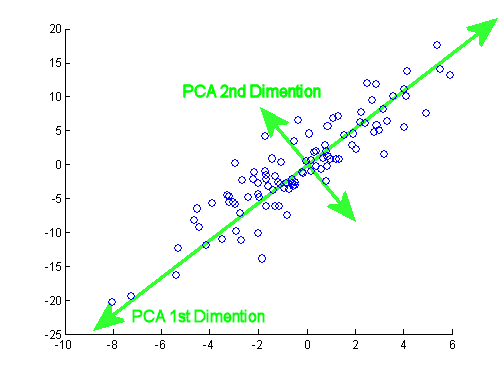
\includegraphics[width=0.5\linewidth]{\toplevelprefix/chapters/chapter1/figs/PCA.png}
    \caption{A distribution with two principal components.}
    \label{fig:PCA}
\end{figure}
The problem is to find the subspace basis $\boldsymbol{U}$ from many samples of $\x$. A typical approach to estimate the subspace $\boldsymbol{U}$ is to minimize the variance of the noise, also known as the minimum mean square error (MMSE):
\begin{equation}
    \min_{\boldsymbol{U}} \mathbb{E}\big[\|\boldsymbol{\epsilon}\|_2^2\big] = \mathbb{E}\big[\|\x - \boldsymbol{U} \z\|_2^2\big].
\end{equation}
Notice that this is essentially a denoising task: once the basis $\boldsymbol{U}$ is correctly found, we can denoise the noisy sample $\x$ by projecting it onto the low-dimensional subspace spanned by $\boldsymbol{U}$ as 
\begin{equation}
\x \rightarrow \hat \x = \boldsymbol{U}\boldsymbol{U}^\top \x. 
\end{equation}
If the noise is small and if we learned the correct low-dimensional subspace $\boldsymbol{U}$, we should expect $\x \approx \hat \x$. That is, PCA is a special case of the auto-encoding:
\begin{equation}
    \x   \xrightarrow{\hspace{2mm} \boldsymbol{U}^\top\hspace{2mm}} \z  \xrightarrow{\hspace{2mm} \boldsymbol{U} \hspace{2mm}} \hat \x.
       \label{eqn:auto-encoding-PCA}
\end{equation}
Only here because of the simple data structure, the encoder $\mathcal{E}$ and decoder $\mathcal{D}$ both become simple linear operators ((projecting and lifting).

This is a classic problem in statistics known as the Principal Component Analysis (PCA). It was first studied by Pearson in 1901 \cite{Pearson1901} and later independently by Hotelling in 1933 \cite{Hotelling1933}. This topic is systematically summarized in the classic book \cite{Jolliffe1986,JolliffeI2002}.
In addition, one may explicitly assume the data $\x$ is distributed according to a single low-dimensional Gaussian:
\begin{equation}
    \x \sim \mathcal{N}(\boldsymbol{0}, \boldsymbol{U}\boldsymbol{U}^\top + \sigma \I), \quad \boldsymbol{U} \in \mathbb{R}^{D\times d},
\end{equation}
which is equivalent to assuming that  $\z$ in the above PCA model \eqref{eqn:PCA-model} is a standard normal distribution. 
This is known as Probabilistic PCA \cite{TippingM1999}. 

In this book, we will revisit  PCA in Chapter \ref{ch:classic}, from the perspective of learning a low-dimensional distribution. Our goal is to use this simple and idealistic model to convey some of the most fundamental ideas for learning a compact representation for a low-dimensional distribution, including the important notion of compression via denoising and autoencoding for a consistent representation.

\paragraph{Independent Component Analysis.}

为了推导卡尔曼滤波器,我们假设系统参数 $(\boldsymbol{A}, \boldsymbol{B}, \boldsymbol{C})$ 是已知的。如果这些参数没有预先给定,问题将更具挑战性,这被称为{\em 系统辨识} (system identification):如何从输入序列 $\{\boldsymbol{u}[n]\}$ 和观测序列 $\{\x[n]\}$ 的(大量样本)中{\em 学习}出参数 $(\boldsymbol{A}, \boldsymbol{B}, \boldsymbol{C})$。这是系统理论中的一个经典问题。如果系统是线性的,可以证明输入和输出序列 $\{\boldsymbol{u}[n], \x[n]\}$ 会共同位于某个低维子空间上\footnote{该子空间的维度与状态空间模型 \eqref{eqn:linear-state-space} 的阶数相同。}。因此,系统辨识问题本质上等价于辨识这个低维子空间 \cite{OverscheeP1996,Liu-2009-CDC,Liu-2010-SIAM}。

值得注意的是,上述问题有两个共同点:第一,(无噪声的)序列或信号被假设是由一个显式的参数化模型族生成的;第二,这些模型本质上都是线性的。因此,从概念上讲,设 $\x_o$ 是一个随机变量,其“真实”分布支撑在一个低维线性子空间(比如 $S$)上。在很大程度上,维纳滤波器和卡尔曼滤波器都是试图从其带噪观测中估计这样的 $\x_o$:
\begin{equation}
    \x = \x_o + \boldsymbol{\epsilon}, \quad \x_o \sim S, 
\end{equation}
其中 $\boldsymbol{\epsilon}$ 通常是随机高斯噪声(或过程)。因此,它们的解法本质上都依赖于辨识一个能够最佳拟合观测(带噪)数据的低维线性子空间。然后,通过将数据投影到这个子空间上,便可以得到最优的去噪操作,且都有闭式解。

%系统理论、信号/图像处理、统计学习和机器学习中的并行发展:如何在高维空间中有效且高效地学习一个更普适的低维分布?线性系统的去噪历史(维纳滤波器和卡尔曼滤波器)。实证

\subsubsection{线性模型与混合线性模型}
\label{sec:PCA-ICA}
\paragraph{主成分分析。}
从上述经典信号处理和系统辨识问题中,我们可以看到,所有这些问题背后的主要任务都是从带噪观测中学习一个{\em 单一}的低维线性子空间。在数学上,我们可以将这种结构建模为:
\begin{equation}
    \x = \boldsymbol{u}_1 z_1 + \boldsymbol{u}_2 z_2 + \cdots + \boldsymbol{u}_d z_d + \boldsymbol{\epsilon} =  \boldsymbol{U} \z + \boldsymbol{\epsilon}, \quad \boldsymbol{U} \in \mathbb{R}^{D\times d}
    \label{eqn:PCA-model}
\end{equation}
其中 $\boldsymbol{\epsilon} \in \mathbb{R}^D$ 是某种微小的随机噪声。图 \ref{fig:PCA} 展示了一个具有两个主成分的此类分布。
\begin{figure}
    \centering
    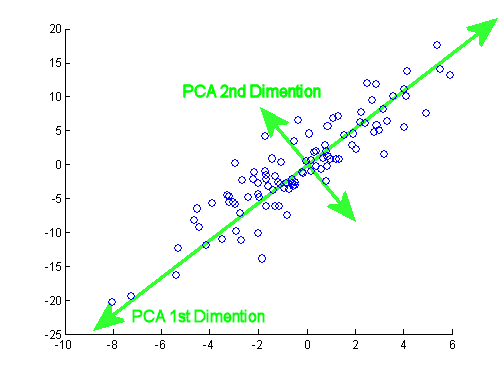
\includegraphics[width=0.5\linewidth]{\toplevelprefix/chapters/chapter1/figs/PCA.png}
    \caption{一个具有两个主成分的分布。}
    \label{fig:PCA}
\end{figure}
问题在于如何从 $\x$ 的大量样本中找出子空间基 $\boldsymbol{U}$。估计子空间 $\boldsymbol{U}$ 的一种典型方法是最小化噪声的方差,这也被称为最小均方误差 (minimum mean square error, MMSE):
\begin{equation}
    \min_{\boldsymbol{U}} \mathbb{E}\big[\|\boldsymbol{\epsilon}\|_2^2\big] = \mathbb{E}\big[\|\x - \boldsymbol{U} \z\|_2^2\big].
\end{equation}
请注意,这本质上是一个去噪任务:一旦正确找到了基 $\boldsymbol{U}$,我们就可以通过将带噪样本 $\x$ 投影到由 $\boldsymbol{U}$ 张成的低维子空间上来对其进行去噪,即
\begin{equation}
\x \rightarrow \hat \x = \boldsymbol{U}\boldsymbol{U}^\top \x. 
\end{equation}
如果噪声很小,并且我们学习到了正确的低维子空间 $\boldsymbol{U}$,那么我们应该期望 $\x \approx \hat \x$。也就是说,PCA 是自编码 (auto-encoding) 的一个特例:
\begin{equation}
    \x   \xrightarrow{\hspace{2mm} \boldsymbol{U}^\top\hspace{2mm}} \z  \xrightarrow{\hspace{2mm} \boldsymbol{U} \hspace{2mm}} \hat \x.
       \label{eqn:auto-encoding-PCA}
\end{equation}
只是在这里,由于数据结构简单,编码器 $\mathcal{E}$ 和解码器 $\mathcal{D}$ 都变成了简单的线性算子(投影和提升)。

这是统计学中的一个经典问题,称为主成分分析 (Principal Component Analysis, PCA)。该问题最早由 Pearson 于 1901 年研究 \cite{Pearson1901},后来 Hotelling 于 1933 年也对其进行了独立研究 \cite{Hotelling1933}。这一主题在经典著作 \cite{Jolliffe1986,JolliffeI2002} 中有系统性的总结。
此外,我们也可以显式地假设数据 $\x$ 服从一个单一的低维高斯分布:
\begin{equation}
    \x \sim \mathcal{N}(\boldsymbol{0}, \boldsymbol{U}\boldsymbol{U}^\top + \sigma \I), \quad \boldsymbol{U} \in \mathbb{R}^{D\times d},
\end{equation}
这等价于假设上述 PCA 模型 \eqref{eqn:PCA-model} 中的 $\z$ 是一个标准正态分布。
这被称为概率主成分分析 (Probabilistic PCA) \cite{TippingM1999}。

在本书中,我们将在第 \ref{ch:classic} 章从学习低维分布的角度重新审视 PCA。我们的目标是利用这个简单而理想化的模型,来传达学习低维分布的紧凑表示的一些最基本的思想,包括通过去噪和自编码实现一致性表示的压缩这一重要概念。

\paragraph{独立成分分析。}

独立成分分析(Independent component analysis, ICA)最初由 \cite{Ans-1985} 提出,作为一种经典的{\em学习良好表示}的模型。事实上,它最初是作为一种关于人类记忆的简单数学模型而提出的。ICA 模型的形式与上述 PCA 模型 \eqref{eqn:PCA-model} 极为相似,该模型假设观测到的随机变量 $\x$ 是多个独立成分 $z_i$ 的线性叠加:
\begin{equation}
    \x = \boldsymbol{u}_1 z_1 + \boldsymbol{u}_2 z_2 + \cdots + \boldsymbol{u}_d z_d  + \boldsymbol{\epsilon} =  \boldsymbol{U} \z + \boldsymbol{\epsilon}.
    \label{eqn:ICA-model}
\end{equation}
然而,此处的成分 $z_i$ 被假设为独立的{\em非高斯}变量。例如,一种常见的选择是
\begin{equation}
    z_i = \sigma_i \cdot w_i, \quad \sigma_i \sim B(1,p),
    \label{eqn:ICA-modes}
\end{equation}
其中 $\sigma_i$ 是一个伯努利随机变量,而 $w_i$ 可以是一个常数值,也可以是另一个随机变量(比如高斯变量)。\footnote{即便 $w$ 是高斯变量,$\sigma w$ 也不再是高斯变量!} ICA 问题旨在从 $\x$ 的观测样本中辨识出 $\boldsymbol{U}$ 和 $\z$。图 \ref{fig:ICA-PCA} 阐释了 ICA 与 PCA 之间的区别。

\begin{figure}
    \centering
    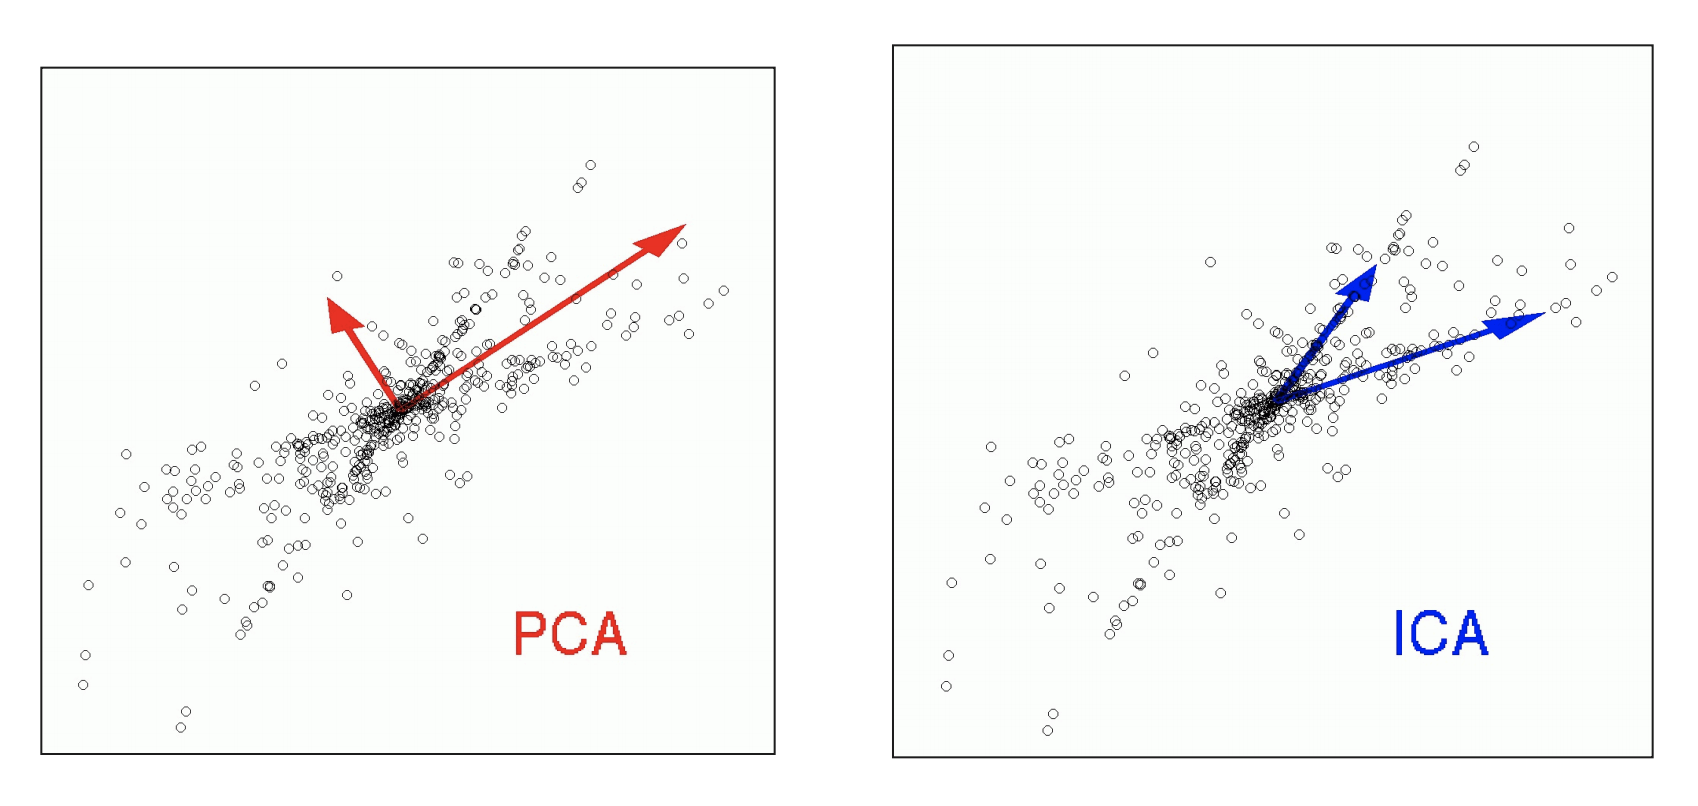
\includegraphics[width=0.7\linewidth]{\toplevelprefix/chapters/chapter1/figs/PCA_ICA.png}
    \caption{PCA(左)与 ICA(右)。}
    \label{fig:ICA-PCA}
\end{figure}

尽管一旦学习得到 $\boldsymbol{U}$ 和 $\z$,从 $\z$ 到 $\x$ 的(解码)映射看似是线性的且易于处理,但从 $\x$ 到 $\z$ 的(编码)映射可能相当复杂,未必能用一个简单的线性映射来表示。因此,ICA 通常得到如下形式的自编码:
\begin{equation}
    \x   \xrightarrow{\hspace{2mm} \mathcal{E}\hspace{2mm}} \z  \xrightarrow{\hspace{2mm} \boldsymbol{U} \hspace{2mm}} \hat \x.
       \label{eqn:auto-encoding-ICA}
\end{equation}
因此,与 PCA 不同,ICA 的分析和求解要困难一些。在 20 世纪 90 年代,以 Erkki Oja 和 Aapo Hyv\"{a}rinen \cite{hyvarinen-1997,Hyvrinen-2000} 为代表的学者们为 ICA 做出了重要的理论和算法贡献。在第 \ref{ch:classic} 章中,我们将研究并给出一个 ICA 的解法,届时编码映射 $\mathcal{E}$ 的含义将变得清晰明了。



\paragraph{稀疏结构与压缩感知。}
我们可以看到,若 \eqref{eqn:ICA-modes} 中的 $p$ 非常小,则任一成分为非零的概率也很小。在这种情况下,我们称 $\x$ 是稀疏生成的,并且它集中在维度为 $k = p \cdot d$ 的一组线性子空间上。因此,在某种程度上,我们可以将上述 ICA 模型推广到一类更普适的、被称为稀疏模型的低维结构。

一个 $k$-稀疏模型定义为所有{\em$k$-稀疏向量}的集合:
\begin{equation}
    \mathcal{Z} = \{\z \in \mathbb{R}^n \mid \|\z\|_0 \le k\},
\end{equation}
其中 $\| \cdot \|_0$ 是 $\ell^0$-范数,表示向量 $\z$ 中非零项的个数。也就是说,$\mathcal{Z}$ 是所有与坐标轴对齐的 $k$ 维子空间的并集,如图 \ref{fig:mixture-models} 左侧所示。在经典信号处理和统计学中,一个重要的问题是如何从其线性观测中恢复稀疏向量 $\z$:

好的,请看翻译结果。

\begin{equation}
    \x = \boldsymbol{A} \z + \boldsymbol{\epsilon}, \quad \boldsymbol{A} \in \mathbb{R}^{m\times n}
    \label{eqn:sparse-model}
\end{equation}
其中 $\boldsymbol{A}$ 为给定矩阵,且通常 $m < n$,$\boldsymbol{\epsilon}$ 为某种微小噪声。这个看似简单的问题,其计算却被证明是 NP-难的,甚至难以近似求解(详情请见专著 \cite{Wright-Ma-2022})。

因此,尽管对此问题的研究历史悠久,最早可追溯至 18 世纪 \cite{Boscovichca1750},但一直没有可被证明有效的算法来解决此类问题,尽管在 20 世纪 60 年代至 90 年代期间,学术界提出并发展了许多启发式算法。其中一些算法在实践中颇为有效,但却缺乏严格的理论依据。21 世纪初,一项重大突破应运而生,当时,包括 David Donoho、Emmanuel Cand\`{e}s 和 Terence Tao 在内的几位著名数学家 \cite{donoho2005neighborly,Candes2005,CandesE2005-IT} 建立了一个严谨的理论框架,该框架使我们能够刻画出稀疏恢复问题得以被有效求解的精确条件,例如,通过凸的 $\ell^1$ 最小化方法:
\begin{equation}
    \min \|\z\|_1 \quad \mbox{subject to} \quad \| \x - \boldsymbol{A}\z\|_2 \le \epsilon,
\end{equation}
其中 $\|\cdot \|_1$ 是促进稀疏性的向量 $\ell^1$ 范数,而 $\epsilon$ 是某个微小的常数。该问题的任何解实质上都给出了一个稀疏编码的映射:
\begin{equation}
    \x   \xrightarrow{\hspace{2mm} \mathcal{E} \hspace{2mm}}  \z.
       \label{eqn:decoding-sparse}
\end{equation}
我们将在第 \ref{ch:classic} 章中简要介绍这种算法,即此种映射,并揭示稀疏编码与深度学习之间有趣的根本性联系。\footnote{尽管早在 2010 年,人们就已注意到稀疏编码算法与深度网络之间的相似性 \cite{gregor2010learning}。}

事实证明,$\ell^1$ 最小化得以成功的条件具有惊人的普适性。成功恢复所需的最小测量数 $m$ 仅与数据的内在维度 $k$ 成正比。这便是如今众所周知的{\em压缩感知}现象 \cite{CandesE2006-ICM}。此外,该现象并不仅限于稀疏结构。它同样适用于非常广泛的低维结构族,例如低秩矩阵等。这些成果从根本上改变了我们对高维空间中低维结构恢复问题的理解。高维数据分析领域的这一戏剧性转折,甚至被 David Donoho \cite{DonohoD2000} 誉为{\em“维数之福”},这与以往处理高维问题时普遍持有的“维数灾难”的悲观信念形成了鲜明对比。这一系列连贯而完备的成果已被系统地整理于专著 \cite{Wright-Ma-2022} 中。

从计算的角度来看,这一新框架的重要性无论如何强调都不为过。它从根本上改变了我们对一类重要问题的看法,而这些问题在过去被认为是基本无法求解的。它使我们能够开发出极其高效的算法,这些算法能够优雅地随问题维度扩展,从而使稀疏恢复问题实现了从:
\begin{equation}
    \mbox{\textbf{难解}} \;
   \Longrightarrow \; \mbox{\textbf{可解}} \; \Longrightarrow \; 
   \mbox{\textbf{可扩展}}。
\end{equation}
这些算法还附带有严格的理论保证,在满足数据和计算的精确要求下,其正确性得以保障。这种方法的严谨与精确性,与主要基于经验的深度神经网络实践几乎截然相反。然而,尽管它们的风格和标准看似迥异,我们现在知道这两种方法共享一个共同目标:{\em 在高维空间中探寻低维结构。}

\paragraph{字典学习。}
从概念上讲,一个比稀疏编码问题 \eqref{eqn:sparse-model} 更为棘手的问题是,观测矩阵 $\boldsymbol{A}$ 事先未知,而我们需要从一组(可能带噪的)观测值(记为 $\X = [\x_1, \x_2, \ldots, \x_n]$)中学习 $\boldsymbol{A}$:
\begin{equation}
    \X = \boldsymbol{A} \Z + \boldsymbol{E}, \quad \boldsymbol{A} \in \mathbb{R}^{m\times n}.
    \label{eqn:dictionary-learning}
\end{equation}
在此问题中,我们只知道 $\X$,而不知道其对应的 $\Z = [\z_1, \z_2, \ldots, \z_n]$ 和噪声项 $\boldsymbol{E}= [\boldsymbol{\epsilon}_1, \boldsymbol{\epsilon}_2, \ldots, \boldsymbol{\epsilon}_n]$,唯一的先验知识是 $\z_i$ 是稀疏的。这就是所谓的{\em 字典学习}问题,它可以被看作是前面讨论过的独立成分分析(ICA)问题 \eqref{eqn:ICA-model} 的一种推广。换句话说,给定数据 $\X$ 的分布是一个标准稀疏分布 $\Z$ 在线性变换 $\boldsymbol{A}$ 下的像,我们希望学习 $\boldsymbol{A}$ 及其“逆”映射 $\mathcal{E}$,从而得到如下的自编码器:
\begin{equation}
    \X   \xrightarrow{\hspace{2mm} \mathcal{E} \hspace{2mm}}  \Z \xrightarrow{\hspace{2mm} \boldsymbol{A} \hspace{2mm}} \X?
       \label{eqn:decoding-DL}
\end{equation}

我们可以看到,主成分分析(PCA)、独立成分分析(ICA)和字典学习的共同之处在于,它们都假设数据分布在低维的线性或混合线性结构附近。它们都要求从可能带噪的分布样本中,学习这些线性结构的(全局或局部)基。在第 \ref{ch:classic} 章中,我们将研究如何通过这些经典模型来识别低维结构。特别是,我们将看到一个有趣而重要的事实:所有这些低维(分段)线性模型都可以通过同一类快速算法——即所谓的{\em 幂迭代}算法 \cite{Zhai-2020}——被有效且高效地学习。尽管对于大多数真实世界的数据而言,上述线性或混合线性模型有些过于简单或理想化,但理解这些模型是通向理解更一般低维分布的重要第一步。

\subsubsection{一般分布}\label{sec:denoising-intro}

诸如图像、视频和音频等真实世界数据的分布极其复杂,难以用上述那些有些理想化的线性模型或高斯过程来建模。我们通常无法{\em 先验地}知道它们是由哪一类参数模型生成的。\footnote{尽管历史上曾有许多尝试为这些数据建立解析模型,例如针对图像数据的随机场或随机过程模型 \cite{Mumford-1999},正如我们在前一节所讨论的那样。} 在实践中,我们通常只拥有其分布的大量样本——即经验分布。显然,在这种情况下,我们通常不能期望为其低维结构或由此产生的去噪算子找到任何闭式解。\footnote{这与主成分分析(PCA)、维纳滤波器和卡尔曼滤波器的情况不同。} 因此,我们需要为这些经验分布开发一种更通用的解决方案,该方案不必是闭式解,但至少是可高效计算的。如果我们处理得当,那么前述那些线性模型的解就应该成为这种通用解的特例。

\paragraph{去噪。}
20世纪50年代,统计学家们开始对任意分布数据的去噪问题产生兴趣。设 $\x_o$ 是一个随机变量,其概率密度函数为 $p_o(\cdot)$。因此,如果我们观测到 $\x_o$ 的一个含噪版本:
\begin{equation}
    \x = \x_o + \sigma \vg, 
\end{equation}
其中 $\vg \sim \dNorm(\vzero, \vI)$ 是标准高斯噪声,$\sigma$ 是观测值的噪声水平。设 $p(\cdot)$ 是 $\x$ 的概率密度函数,\footnote{也就是说,$p(\x) = \int_{-\infty}^{\infty} \phi_{\sigma}(\x - \z)p_o(\z) \odif{\z}$,其中 $\phi_{\sigma}$ 是高斯分布 $\mathcal{N}(\boldsymbol{0}, \sigma^2 \boldsymbol{I})$ 的密度函数。} 令人惊奇的是,给定 $\x$ 的条件下 $\x_o$ 的后验期望可以通过一个优美的公式计算得出,这个公式被称为特威迪公式(Tweedie's formula)\cite{Robbins1956AnEB}:\footnote{赫伯特·罗宾斯(Herbert Robbins)在个人通信中表示,该公式的功劳应归于莫里斯·肯尼思·特威迪(Maurice Kenneth Tweedie)。}
\begin{equation}
    \hat \x_o = \mathbb{E}[\x_o\mid \x] = \x + \sigma^2 \nabla \log p(\x).
\end{equation}
从该公式中可以看出,函数 $\nabla \log p(\x)$ 在对观测值 $\x$ 进行去噪时扮演着一个非常特殊的角色。噪声 $\vg$ 可以被显式地估计为
\begin{equation}
    \hat{\vg} = \frac{\x - \hat \x_o}{\sigma} = -\sigma \nabla \log p(\x),
\end{equation}
为此,我们只需要知道 $\x$ 的分布 $p(\cdot)$,而不需要知道 $\x_o$ 的真实分布 $p_o(\cdot)$。该结果的一个重要启示是,如果我们向任何分布添加高斯噪声,只要我们能以某种方式获得函数 $\nabla \log p(\x)$,去噪过程就可以轻松完成。

由于这是一个非常重要且有用的结果,它在许多不同的背景和领域中被反复重新发现和使用。例如,在特威迪公式 \cite{Robbins1956AnEB} 之后几年,\cite{Miyasawa61} 又重新发现了它。21世纪初,函数 $\nabla \log p(\x)$ 在学习通用分布的背景下再次被重新发现,并被阿普·海瓦里宁(Aapo Hyv\"{a}rinen)命名为“分数函数”(score function)\cite{hyvarinen05a}。但它与(经验贝叶斯)去噪的联系很快被 \cite{Vincent2011} 所认识到。
埃罗·西蒙切利(Eero Simoncelli)的研究小组 \cite{Raphan10} 将其推广到了其他测量分布(高斯噪声之外),后来又应用于图像去噪 \cite{Kadkhodaie21a,ho2020denoising}。

\begin{figure}
    \centering
    %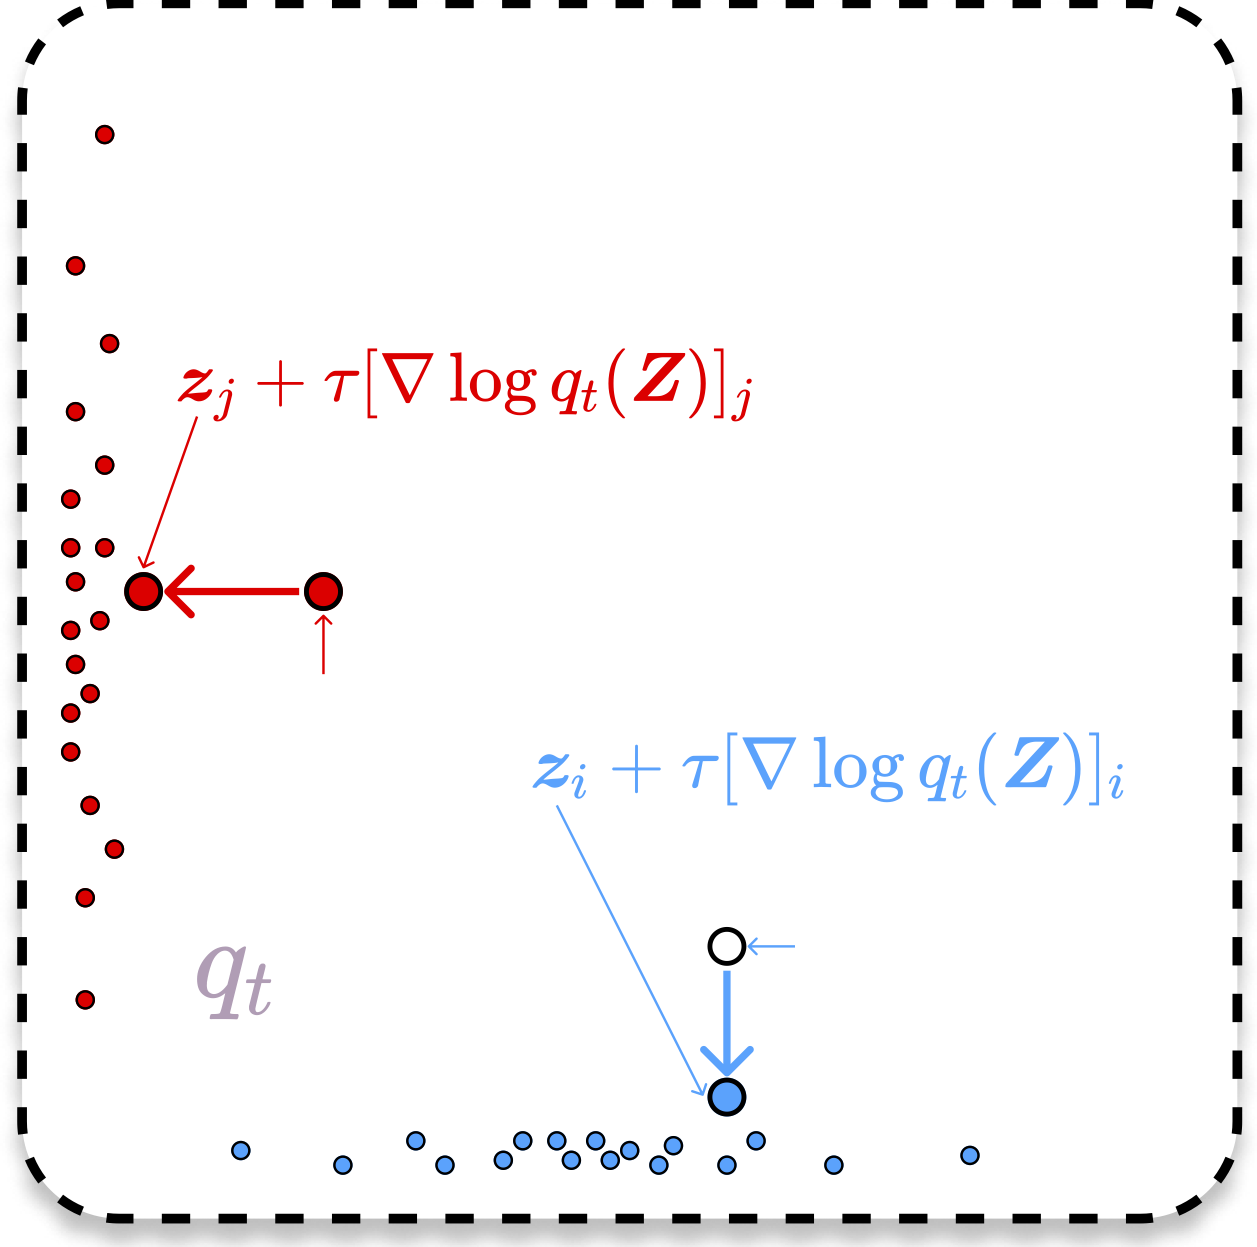
\includegraphics[width=0.45\linewidth]{\toplevelprefix/chapters/chapter1/figs/Score.png}
    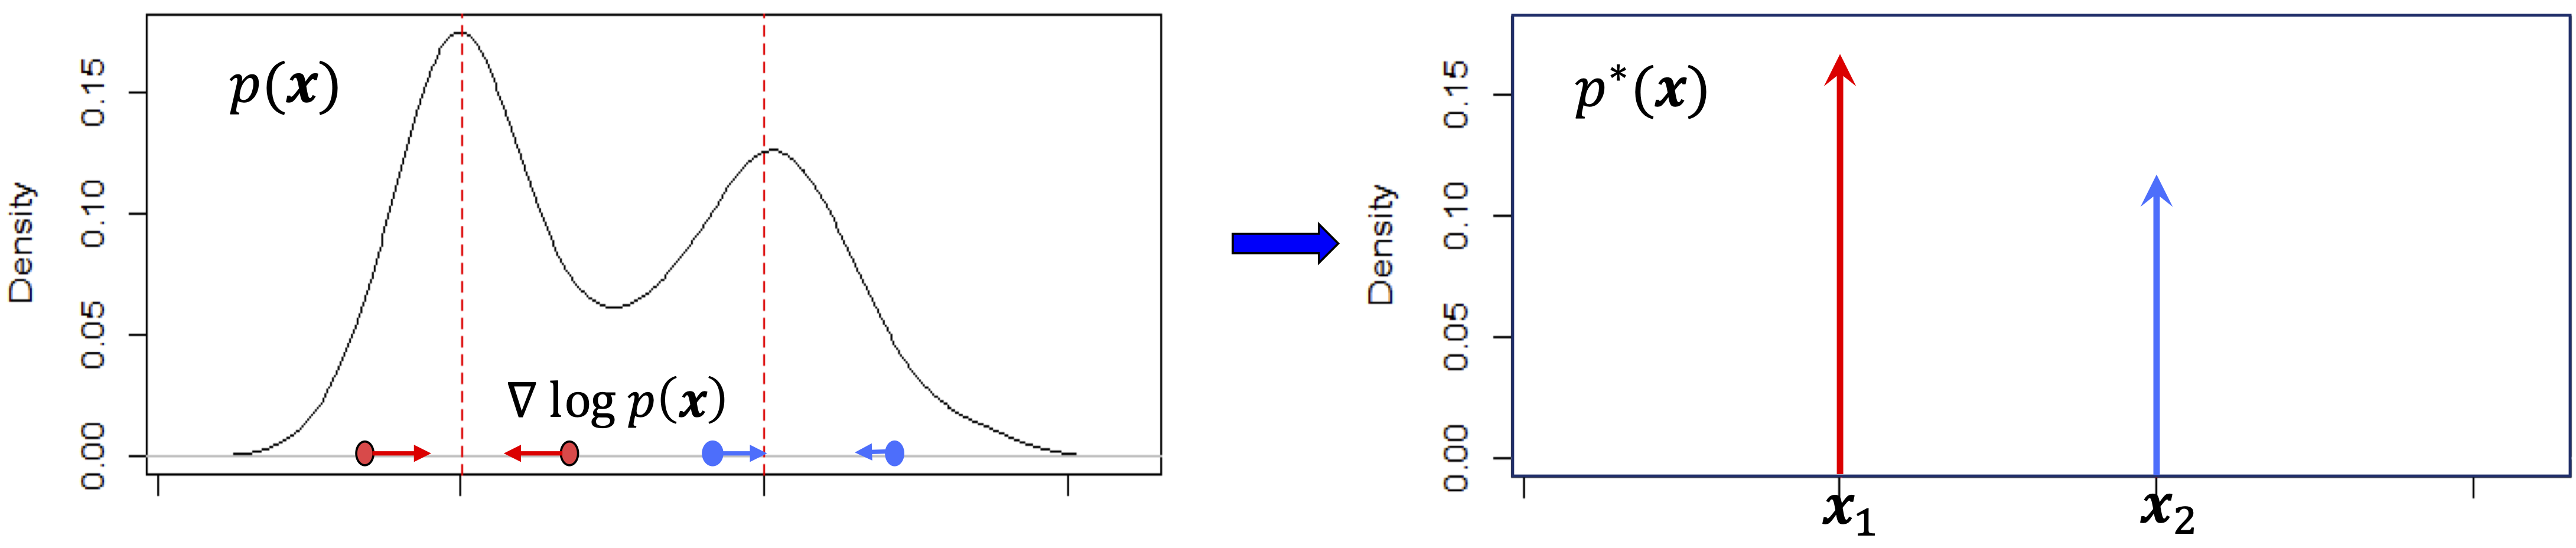
\includegraphics[width=1\linewidth]{\toplevelprefix/chapters/chapter1/figs/Density-compress.png}
    \caption{分数函数 $\nabla \log p(\x)$ 的几何解释。左图展示了一个密度为 $p(\x)$ 的分布。由分数函数生成的操作将分布推向密度更高的区域。其目标是,通过某种紧凑性度量(例如熵或编码长度),使最终得到的分布更加“压缩”。最终,该分布会收敛到一个具有更低维度支撑集的分布,如右图所示的 $p^*(\x)$。}
    \label{fig:score-function}
\end{figure}

\paragraph{熵最小化。}

事实上,该函数具有一个非常直观的信息论与几何解释。注意,在信息论中,$-\log p(\x)$ 通常对应于编码 $\x$ 所需的比特数\footnote{至少在离散变量的情况下是如此,我们将在第 \ref{ch:compression} 章中对此进行更详细的解释。}。梯度 $\nabla \log p(\x)$ 指向密度更高的方向,如图 \ref{fig:score-function} 左侧所示。如果 $\x$ 沿该方向移动,编码它所需的比特数就会减少。因此,算子 $\nabla \log p(\x)$ 的整体效果是推动分布向密度更高的区域“收缩”。实际上,我们可以严格证明,分布的(微分)熵
\begin{equation}
H(\x) = - \int p(\boldsymbol{w}) \log p(\boldsymbol{w}) \odif{\boldsymbol{w}}    \end{equation} 
在此类操作下确实会减小(参见第 \ref{ch:compression} 章和附录 \ref{app:diffusion-denoising})。因此,如果我们用最优码本对其进行编码,所得分布的总编码长度/率会降低,从而变得更加“压缩”。直观上可以想象,如果我们无限次重复这样的去噪过程,分布最终将收缩为一个其质量集中在更低维度支撑集上的分布。例如,如图 \ref{fig:score-function} 左侧所示的分布 $p(\x)$,在分数函数 $\nabla \log p(\x)$ 的作用下,最终将收敛到右侧的分布 $p^*(\x)$\footnote{严格来说,$p^*(\x)$ 是一个其密度为广义函数的分布:$p^*(\x) = p^*(\x_1)\delta(\x-\x_1) + p^*(\x_2) \delta(\x-\x_2)$,且满足 $p^*(\x_1) + p^*(\x_2) = 1$。}:
\begin{equation}
H(\x) = - \int p(\boldsymbol{w}) \log p(\boldsymbol{w}) \odif{\boldsymbol{w}}  \quad \xrightarrow{\hspace{1mm} \mbox{递减} \hspace{1mm}} \quad H^*(\x) = - \int p^*(\boldsymbol{w}) \log p^*(\boldsymbol{w}) \odif{\boldsymbol{w}}.    
\end{equation}
严格来说,随着分布收敛到 $p^*(\x)$,其微分熵会收敛到负无穷大。这归因于连续随机变量与离散随机变量的微分熵定义之间的一个技术性差异。我们将在第 \ref{ch:compression} 章中看到如何使用一个更统一的度量,即{\em 率失真},来解决这个技术难题。


我们将在本章的后续部分以及第 \ref{ch:compression} 章中讨论,这样一个看似简单的去噪和压缩概念,如何引出一种非常统一且强大的方法,用于学习高维空间中的普遍低维分布,包括自然图像的分布。

\subsection{经验方法}

在实践中,对于许多重要的现实世界数据,如图像、声音和文本,很难用理想化的线性或混合线性模型来对其进行建模。例如,在图像处理和计算机视觉领域,研究者们曾长期致力于对自然图像的分布进行解析建模,并积累了丰硕的成果。菲尔兹奖得主大卫·芒福德(David Mumford)在20世纪90年代投入了大量精力,试图理解和建模自然图像的统计特性 \cite{Mumford1996TheSD}。他与他的学生们,包括朱松纯(Song-Chun Zhu),从统计物理学中汲取灵感和技术,为自然图像的分布提出了许多统计和随机模型 \cite{Zhu-Entropy-1997,Zhu1997LearningGP,Zhu1997Prior,Huang-Mumford,Mumford-1999,Lee-Mumford}。然而,这些解析模型在生成与自然图像高度相似的样本方面,收效甚微。显然,对于像图像这样的现实世界数据,我们需要发展更强大、更统一的方法,以探寻其更普遍的低维结构。

因此,在历史上,许多经验模型被提出来用于建模重要的现实世界数据,包括图像和文本。这些模型常常从生物神经系统的特性中汲取灵感,因为动物或人类的大脑似乎能够极其高效地处理这些数据。

\subsubsection{经典人工神经网络}
\paragraph{人工神经元。}

\begin{figure}[t]
    \centering
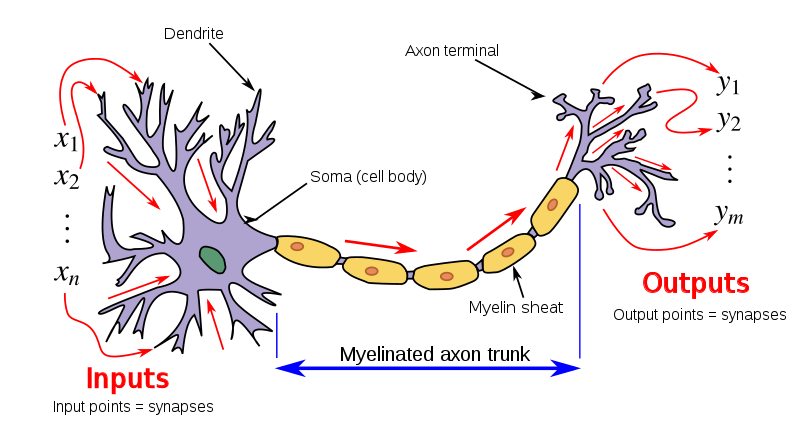
\includegraphics[width=0.55\linewidth]{\toplevelprefix/chapters/chapter1/figs/neuron.png} \hspace{3mm}   
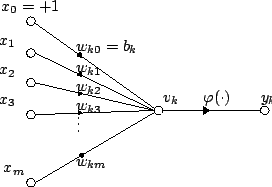
\includegraphics[width=0.40\linewidth]{\toplevelprefix/chapters/chapter1/figs/Artificial_neuron.png}
    \caption{首个模仿神经元(左)处理信号方式的人工神经元(右)的数学模型。}
    \label{fig:neuron}
\end{figure}

受大脑神经系统的启发,沃伦·麦卡洛克(Warren McCulloch)\footnote{时任芝加哥大学精神病学教授}和沃尔特·皮茨(Walter Pitts)于1943年提出了第一个人工神经元\footnote{被称为线性阈值单元(Linear Threshold Unit),或感知机(perceptron)。}的数学模型 \cite{McCulloch-Pitts}。该模型描述了输入 $x_i$ 和输出 $o_j$ 之间的关系如下:
\begin{equation}
    o_j = \varphi\Big( \sum_i w_{ji}x_i\Big),  
\end{equation}
其中 $\varphi(\cdot)$ 是某种非线性激活函数,通常被建模为阈值函数。该模型如图 \ref{fig:neuron} 所示。我们可以看到,这种形式已经具备了现代深度神经网络中基本单元的主要特征。该模型源于对我们神经系统中单个神经元工作方式的观察。然而,当时人们并不确切知道由这样一组神经元构成的集合,想要实现和执行何种功能。在更技术的层面上,他们也不确定应该使用哪种非线性激活函数 $\varphi(\cdot)$。因此,历史上提出了许多变体。\footnote{阶跃函数、硬阈值或软阈值函数、修正线性单元(ReLU)、Sigmoid函数等。}

\begin{figure}[t]
\centering
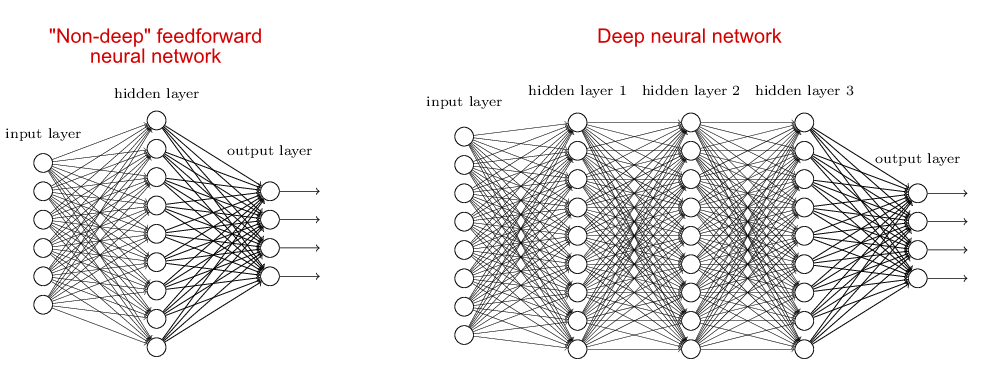
\includegraphics[width=0.85\linewidth]{\toplevelprefix/chapters/chapter1/figs/single-deep.png}
    \caption{单隐藏层网络(左)与深度网络(右)的对比。}
    \label{fig:single-deep}
\end{figure}
\paragraph{人工神经网络。}
在20世纪50年代,弗兰克·罗森布拉特(Frank Rosenblatt)首次构建了一台由这种人工神经元组成的{\em 网络}机器,如图 \ref{fig:perceptron} 所示。这台机器被称为马克一号感知机(Mark I Perceptron),它由一个输入层、一个输出层和一个包含512个人工神经元的单隐藏层组成,如图 \ref{fig:perceptron} 左图所示,其结构与图 \ref{fig:single-deep} 左图所展示的类似。它被设计用来对字母的光学图像进行分类。然而,单层网络的能力有限,只能学习线性可分的模式。在1969年马文·明斯基(Marvin Minsky)和西摩尔·派普特(Seymour Papert)合著的《感知机:计算几何导论》({\em Perceptrons: An Introduction to Computational Geometry})一书中 \cite{Minsky-1969},证明了马克一号感知机的单层结构无法学习异或(XOR)函数。这一结果极大地削弱了人们对人工神经网络的兴趣,尽管后来证明多层网络能够学习异或函数 \cite{Rumelhart1986}。事实上,一个(足够大的)由这类简单神经元组成的多层网络,如图 \ref{fig:single-deep} 右图所示,可以模拟任何有限状态机,甚至是通用图灵机。\footnote{不应将神经网络在原理上能做什么,与学习一个实现特定期望功能的神经网络是否易于处理或简单相混淆。} 尽管如此,人工神经网络的研究在随后的20世纪70年代进入了它的第一个寒冬。

\begin{figure}
    \centering
    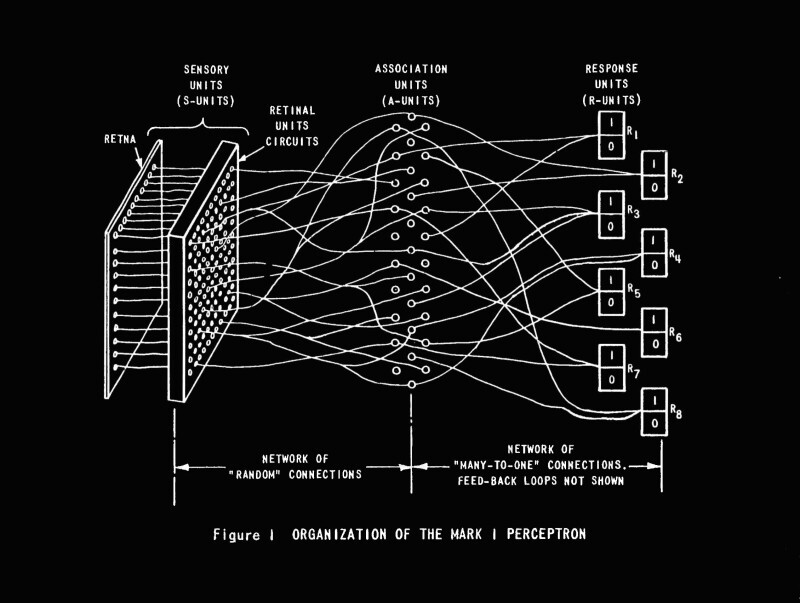
\includegraphics[width=0.45\linewidth]{\toplevelprefix/chapters/chapter1/figs/visu-large.jpg}
    \hspace{2mm} 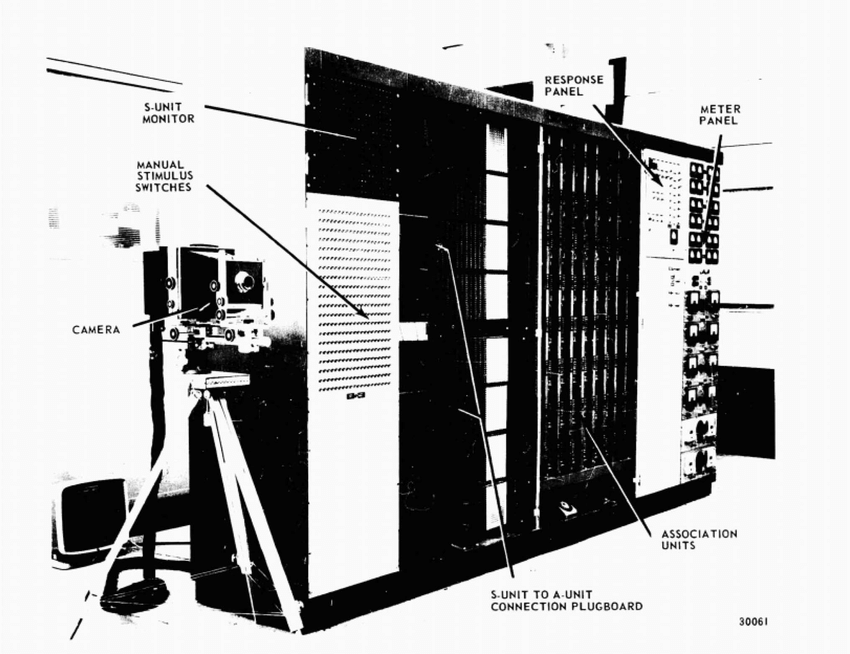
\includegraphics[width=0.45\linewidth]{\toplevelprefix/chapters/chapter1/figs/Original-Mark-I-perceptron-as-seen-in-its-operators-manual-20.ppm.png}
    \caption{弗兰克·罗森布拉特于20世纪50年代末开发的马克一号感知机。}
    \label{fig:perceptron}
\end{figure}


\paragraph{卷积神经网络。}

20世纪50至60年代,类似马克一号感知器(Mark I Perceptron)这样的人工神经网络的早期实验结果不尽人意,这表明,仅仅以多层感知器(MLP)的通用方式连接神经元或许是不足够的。为了构建有效且高效的网络,我们需要理解网络中的神经元需要共同实现何种目的或功能,从而以某种特殊的方式对其进行组织和学习。于是,机器智能的研究再次转向,从动物的神经系统如何工作中汲取灵感。

众所周知,我们大脑的大部分区域都用于处理视觉信息。在20世纪50至60年代,戴维·休伯尔(David Hubel)和托斯坦·威泽尔(Torsten Wiesel)系统地研究了猫的视觉皮层。他们发现,视觉皮层包含不同类型的细胞(被称为简单细胞和复杂细胞),这些细胞对不同方向和位置的视觉刺激很敏感 \cite{Hubel-Wiesel-1959}。因其开创性的发现,休伯尔和威泽尔荣获了1981年的诺贝尔生理学或医学奖。


在人工神经网络方面,休伯尔和威泽尔的研究启发了福岛邦彦(Kunihiko Fukushima)。他在1980年设计了“新认知机”(neocognitron)网络,该网络由模拟视觉皮层中生物神经元的人工神经元组成 \cite{Fukushima1980NeocognitronAS}。这被认为是第一个{\em 卷积神经网络}(CNN),其架构如图\ref{fig:neocognitron}所示。与感知器不同,新认知机拥有不止一个隐藏层,可以被视为一种深度网络,如右图\ref{fig:single-deep}的比较所示。

同样受到猫视觉皮层神经元工作方式的启发,他也率先引入了{\em 修正线性单元}(ReLU):
\begin{equation}
    \varphi(x) = \max\{0, x\} = \casework{x, & \text{if} \, x > 0, \\ 0, \quad & \text{if} \, x \leq 0,}
\end{equation}
作为1969年的激活函数 $\varphi(\cdot)$ \cite{Fukushima-1969}。但直到近年,ReLU才成为现代深度(卷积)神经网络中广泛使用的激活函数。在本书中,当我们解释了深度网络试图实现的主要操作——压缩之后,我们将了解到为何这是一个很好的选择。
%\yima{此处应有一张卷积神经网络或LeNet的图片...}

\begin{figure}
    \centering
    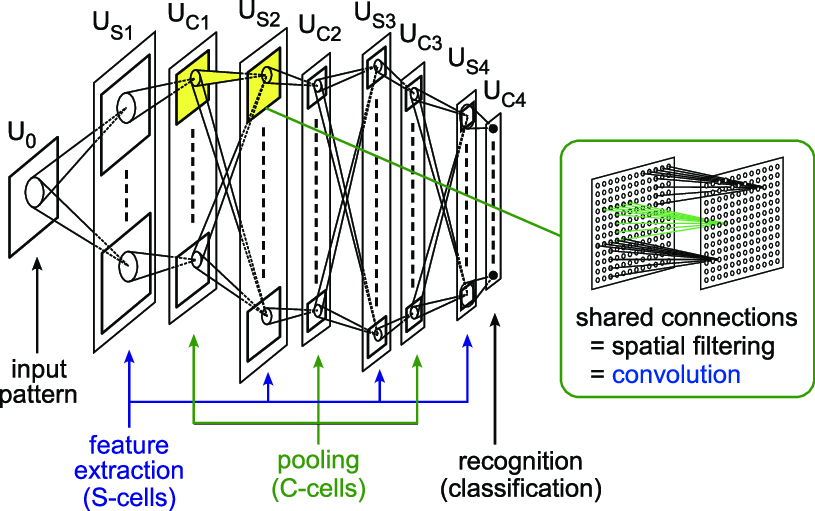
\includegraphics[width=0.6\linewidth]{\toplevelprefix/chapters/chapter1/figs/neocognitron.png}
    \caption{卷积神经网络的起源:由福岛邦彦于1980年提出的新认知机。请注意,卷积层和池化层的交替排布,旨在模拟在猫的视觉皮层中发现的简单细胞和复杂细胞的功能。}
    \label{fig:neocognitron}
\end{figure}

在20世纪80年代,类CNN网络不断发展,许多不同的变体被相继提出和研究。然而,尽管深度网络具有卓越的能力,且其架构受到神经科学的启发而得以改进,但要为一个诸如图像分类的真实任务训练这样的深度网络,依然是极其困难的。如何让一个网络有效工作,依赖于许多无法解释的启发式方法和技巧,这极大地限制了神经网络的吸引力和适用性。大约在1989年,一项重大突破出现:杨立昆(Yann LeCun)成功地使用{\em 反向传播}(BP)算法来训练一个用于识别手写数字的深度卷积神经网络 \cite{LeCun-1989},这个网络后来被称为LeNet(见图\ref{fig:LeNet-5})。经过数年坚持不懈的研发,他的毅力终获回报:在20世纪90年代末,LeNet的性能终于达到了足以实际应用的水平 \cite{LeCun-1998}:它被美国邮政局用于识别手写数字(邮政编码)。LeNet被认为是所有现代深度神经网络的“原型”网络,例如我们稍后将要讨论的AlexNet和ResNet。由于这项工作,杨立昆荣获了2018年的图リング奖。\footnote{与另外两位深度网络的先驱约书亚·本吉奥(Yoshua Bengio)和杰弗里·辛顿(Geoffrey Hinton)共同获奖。}

\begin{figure}
    \centering
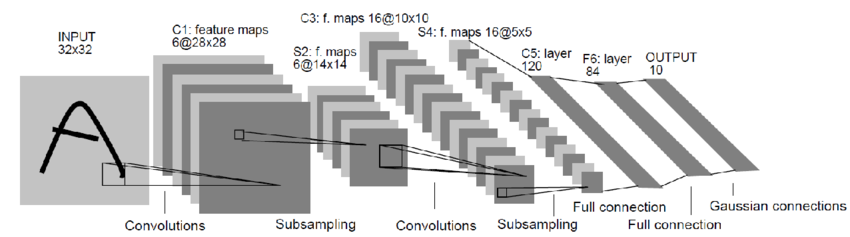
\includegraphics[width=0.95\linewidth]{\toplevelprefix/chapters/chapter1/figs/LeNet-5.png}
    \caption{由 Yann LeCun 于 1989 年设计的 LeNet-5 卷积神经网络。}
    \label{fig:LeNet-5}
\end{figure}

\paragraph{反向传播。}
回顾历史,深度神经网络的命运似乎与其能否被便捷高效地训练这一问题息息相关。反向传播(Backpropagation, BP)算法正是为此而生。我们知道,多层感知机可以表示为一系列线性映射与非线性激活的复合,其形式如下:
\begin{equation}
h(\bm W_1, \ldots, \bm W_L) = f^L(\bm W_Lf^{L-1}(\bm W_{L-1} \cdots f^2(\bm W_2f^1(\bm W_1\x)))).
\end{equation}
为了基于梯度下降算法训练网络权重 $\{\bm W_l\}_{l=1}^L$ 以降低预测或分类误差,我们需要计算梯度 ${\partial h}/{\partial \bm W_l}$。根据微积分中的{\em链式法则},我们早已知晓,对于此类函数,其梯度可以被高效地计算,这种方法后来便被称为反向传播(BP)算法。详细描述参见附录 \ref{app:optimization}。早在 20 世纪 60 年代和 70 年代,反向传播技术就已为最优控制和动态规划等领域的学者所熟知并付诸实践。例如,该技术出现在 Paul Werbos 博士 1974 年的博士论文中 \cite{Werbos-1974, Werbos1994TheRO}。1986 年,David Rumelhart 等人首次将反向传播算法应用于训练多层感知机(MLP)网络 \cite{Rumelhart1986}。从那时起,BP 算法便日益普及,因为它为学习大型深度神经网络提供了一种{\em可扩展的}算法。\footnote{因为它可以在支持并行和分布式计算的平台上高效实现。} 如今,它已成为训练深度神经网络的一项近乎主导性的技术。然而,人们普遍认为,自然界并非通过反向传播进行学习,因为对于自然界来说,物理实现这种机制的代价仍然过于高昂\footnote{正如我们前面所讨论的,自然界几乎普遍通过闭环反馈来纠正错误从而进行学习。}。这显然为未来的发展留下了巨大的改进空间,我们稍后将对此进行更深入的探讨。

然而,尽管 20 世纪 80 年代在算法上取得了上述进展,实践上也展现了光明的前景,但在 80 年代和 90 年代,对于当时的计算系统而言,训练深度神经网络仍然是一项极其繁琐且代价高昂的任务。在 20 世纪 90 年代末,支持向量机(SVM)\cite{SVM-1995} 开始广受欢迎,因为在分类等任务上,它被认为是比神经网络更好的替代方案。\footnote{事实上,解决分类问题的类似思想可以追溯到 Thomas Cover 的博士论文工作,其精简版本已于 1964 年发表在一篇论文中 \cite{Cover-1964}。} 这主要有两个原因:其一,SVM 基于一个被称为 Vapnik–Chervonenkis(VC)理论的严谨统计学习框架;其二,它可以导出基于凸优化的高效算法 \cite{BoydVa04}。SVM 的兴起,为神经网络的研究在 21 世纪初带来了第二次寒冬。

\paragraph{压缩自编码。}

早在20世纪80年代末至90年代,人工智能神经网络就已被用于学习图像等高维数据的低维表示。研究表明,神经网络可以用于从数据中学习主成分分析(PCA)\cite{Oja1982SimplifiedNM,Baldi89},以替代第 \ref{sec:PCA-ICA} 节中讨论的经典方法。同样在80年代末期,有学者提出,鉴于神经网络能够对非线性变换进行建模,可利用其学习非线性分布数据的低维表示。与线性PCA的情形类似,我们可以尝试同时学习一个非线性降维编码器 $f$ 和一个解码器 $g$,并用深度神经网络对二者进行建模 \cite{Rumelhart1986,Kramer1991NonlinearPC}:
\begin{equation}
    \X   \xrightarrow{\hspace{2mm} f \hspace{2mm}} \Z  \xrightarrow{\hspace{2mm} g \hspace{2mm}} \hat \X.
       \label{eqn:auto-encoding-deep-networks}
\end{equation}
通过强制解码数据 $\hat \X$ 与原始数据 $\X$ 保持一致,例如,通过最小化最小均方误差(MMSE)类型的重构误差\footnote{尽管众所周知,对于具有复杂非线性结构的图像数据,最小均方误差类型的误差函数存在问题。正如我们稍后将讨论的,包括生成对抗网络(GAN)在内的许多近期生成方法研究,一直致力于为原始数据 $\X$ 和生成数据 $\hat \X$ 之间寻找更好的距离函数替代方案。}:
\begin{equation}
    \min_{f,g} \big\|\X - \hat \X\big\|_2^2 = \big\|\X - g(f( \X))\big\|_2^2,
\end{equation}
我们便可以从数据 $\X$ 本身学习到一个自编码器。

但是,我们如何能保证这种自编码确实捕捉了 $\X$ 中真实的低维结构,而不是给出一个平凡的冗余表示呢?例如,我们可以简单地选择 $f$ 和 $g$ 为恒等映射,此时 $\Z = \X$。因此,为确保自编码的价值,我们希望得到的表示在某种可计算的复杂度度量下是压缩的。1993年,Geoffrey Hinton及其同事提出使用编码长度作为这样的度量,因此自编码的目标就变成了寻找能够最小化编码长度的表示 \cite{Hinton-1993}。这项工作还在最小描述长度原理 \cite{Rissanen-1978} 和自由能(亥姆霍兹自由能)最小化之间建立了根本性的联系。Hinton团队后来的工作 \cite{Hinton504} 通过实验表明,这种自编码能够为真实世界的图像学习到有意义的低维表示。就在深度网络开始流行之前,Pierre Baldi 于2011年对自编码器做了一次较为全面的综述 \cite{Baldi2011}。我们将在第 \ref{sec:unifying-approach} 节中进一步讨论复杂度的度量和自编码,并在第 \ref{ch:consistent} 章中以一个更统一的视角对压缩自编码进行系统性的研究。


\begin{figure}
    \centering
    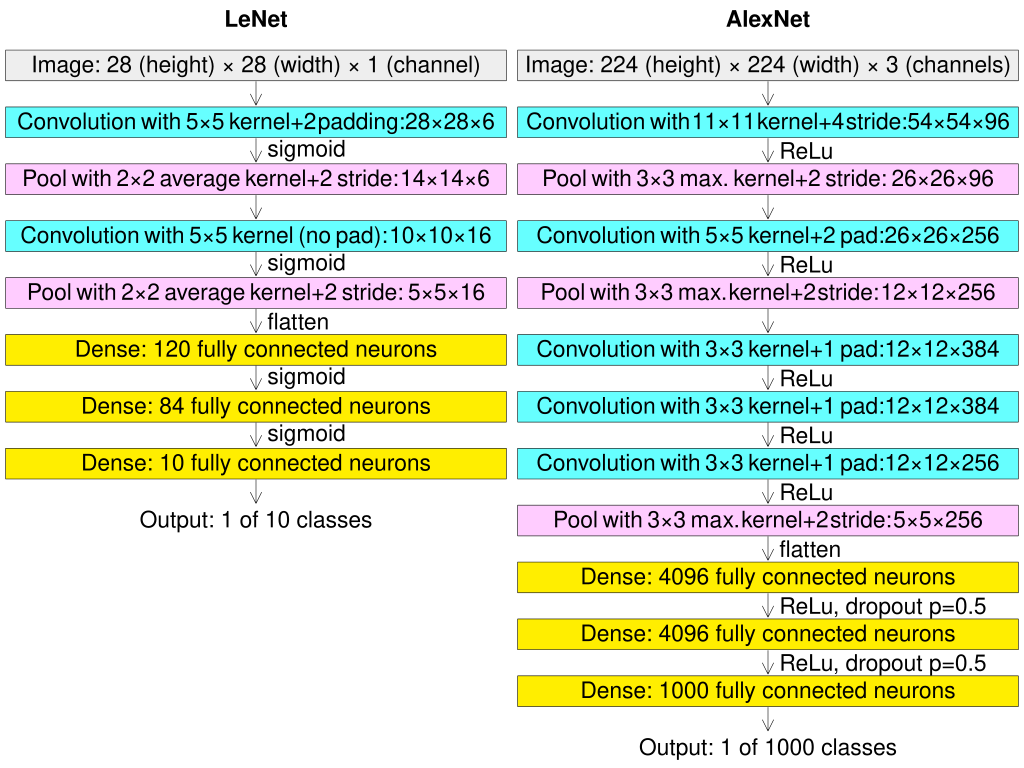
\includegraphics[width=0.8\linewidth]{\toplevelprefix/chapters/chapter1/figs/Comparison_image_neural_networks.svg.png}
    \caption{LeNet \cite{LeCun-1989} 与 AlexNet \cite{krizhevsky2012imagenet} 的架构对比。}
    \label{fig:LeNet-AlexNet}
\end{figure}


\subsubsection{现代深度神经网络}
从20世纪80年代到21世纪10年代,在长达近30年的时间里,主流的机器学习和机器智能研究并未对神经网络给予足够重视。早期的(深度)神经网络,如LeNet,在识别数字等小规模分类问题上展现了良好的性能潜力。然而,当时神经网络的设计和实践相当依赖经验,可用的数据集规模很小,而且反向传播(BP)算法对当时的计算机而言是巨大的计算负担。这些因素导致了学界对神经网络缺乏兴趣,研究进展停滞不前,只有少数研究人员坚持在这一领域工作。

\paragraph{分类与识别。}
事实证明,只有当数据和算力足够充分时,深度神经网络的巨大潜力才能被释放出来。时间快进到21世纪10年代,ImageNet等更大型的数据集面世,图形处理器(GPU)也变得足够强大,使得反向传播算法的成本大大降低,即便是对于比LeNet大得多的网络也同样如此。2012年前后,一个名为AlexNet的深度卷积神经网络引起了广泛关注,因为它在ImageNet数据集上的表现以显著优势超越了当时已有的分类方法 \cite{krizhevsky2012imagenet}。\footnote{事实上,在此之前,深度网络已在语音识别任务中展现出顶尖水平的性能。但直到其在图像分类上取得成功,才获得了如此广泛的关注。} 图 \ref{fig:LeNet-AlexNet} 展示了AlexNet和LeNet的对比。AlexNet与LeNet有许多共同特征,只是规模更大,并且采用了ReLU作为非线性激活函数,而非LeNet中使用的Sigmoid函数。Geoffrey Hinton在2018年荣获图灵奖,部分原因也是受此项工作的影响。

这一早期的成功激励了机器智能领域的研究者们在接下来的几年里探索网络设计的各种新变体和改进。特别是,人们通过经验发现,网络越大越深,在图像分类等任务中的性能就越好。许多深度网络架构被相继提出、测试并推广。其中一些著名的架构包括VGG \cite{Simonyan15}、GoogLeNet \cite{Szegedy2014GoingDW}、ResNet \cite{He2016-lc},以及近期的Transformers \cite{vaswani2017attention} 等。尽管在经验性能上取得了快速进展,但对于这些凭经验发现的架构,学界仍缺乏理论上的解释,包括它们之间可能存在的内在联系。本书的目的之一,便是揭示所有这些网络可能服务的共同目标,并阐释为何它们会共享某些共通特性,例如多层线性算子与非线性激活函数交错的结构(见第 \ref{ch:representation} 章)。

\paragraph{强化学习。}

深度网络早期的成功主要集中于监督学习环境下的分类任务,例如语音识别和图像识别。之后,由 Demis Hassabis 领导的 DeepMind 团队采用深度网络来学习玩游戏的决策或控制策略。在此背景下,深度网络被用来建模最优决策/控制策略或相关的最优价值函数,如图 \ref{fig:Alpha-Go} 所示。这些网络参数基于当前策略在游戏中的成败所返回的奖励,进行增量式优化\footnote{例如基于反向传播 (BP) 算法。}。这种学习方法通常被称为{\em 强化学习} \cite{Sutton-Barto},它起源于 20 世纪 60 年代末的控制系统实践 \cite{Waltz1965AHA,Mendel1970ReinforcementlearningCA}。其更早的渊源可以追溯到 20 世纪 50 年代,历史更为悠久和丰富的 Richard Bellman 的{\em 动态规划} \cite{Bellman-DP} 和 Marvin Minsky 的{\em 试错学习} \cite{Minsky-1954}。

从实现的角度来看,深度网络与强化学习的结合被证明相当强大:深度网络可以用来近似那些难以进行解析建模的真实世界环境中的控制策略和价值函数。这一实践最终催生了由 DeepMind 公司开发的 AlphaGo 系统。该系统于 2016 年击败了顶尖人类棋手李世石 (Lee Sedol),并于 2017 年战胜了世界冠军柯洁 (Jie Ke),在围棋比赛中震惊了世界。\footnote{1996年,IBM 的“深蓝”(Deep Blue) 系统在国际象棋比赛中击败俄罗斯特级大师加里·卡斯帕罗夫 (Garry Kasparov),创造了历史。它主要使用的是传统的机器学习技术,如树搜索和剪枝,这些技术的可扩展性不强,并且在之后 20 多年的时间里,也未能证明其可成功应对像围棋这样更具挑战性的游戏。}

AlphaGo 的成功令整个计算机学界大为震惊,因为学界普遍认为围棋的搜索状态空间大到望而却步,无论是在计算量还是样本量方面,都不可能存在任何有效的解决方案。对其成功唯一合理的解释是,围棋游戏的最优价值/策略函数中必定存在非常好的结构。它们的内在维度并不那么高,因此可以用一个神经网络很好地近似,并且可以从并非多到不可行的样本中学习得到。

\begin{figure}
    \centering
    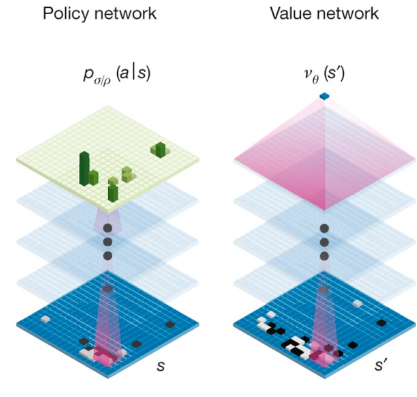
\includegraphics[width=0.5\linewidth]{\toplevelprefix/chapters/chapter1/figs/Policy-Value.png}
    \caption{AlphaGo:使用深度神经网络为围棋游戏建模最优策略或最优价值函数。}
    \label{fig:Alpha-Go}
\end{figure}

\paragraph{生成与预测。}
我们可以认为,21 世纪 10 年代深度网络的早期实践更侧重于从数据 $\X$ 中提取相关信息,并将其编码为某种特定于任务的表示 $\Z$(例如,在分类任务中,$\Z$ 代表类别标签):
\begin{equation}
    \X   \xrightarrow{\hspace{2mm} f \hspace{2mm}} \Z.
       \label{eqn:encoding-deep-networks}
\end{equation}
在这种设定下,所要学习的映射 $f$ 无需保留 $\X$ 的大部分分布信息,而只需保留特定任务所需的充分统计量。例如,$\X$ 中的一个样本 $\x$ 可能是一张苹果的图像,它通过 $f$ 映射到其类别标签 $\z =$ “苹果”。2015 年提出的{\em 信息瓶颈框架} \cite{Tishby-ITW2015} 正是为了分析深度网络在此类背景下的作用。
 
然而,在许多现代场景中,例如在所谓的“大型基础模型”中,人们常常需要解码 $\Z$ 以在一定精度上恢复相应的 $\X$:
\begin{equation}
    \Z   \xrightarrow{\hspace{2mm} g  \hspace{2mm}} \hat \X.
       \label{eqn:decoding-deep-networks}
\end{equation}
由于 $\X$ 通常代表从外部世界观测到的数据,一个好的解码器将使我们能够模拟或预测世界上发生的事情。例如,在“文本到图像”或“文本到视频”任务中,$\z$ 通常代表描述所需图像 $\x$ 内容的文本。解码器应该能够生成一个与 $\x$ 内容相同的 $\hat \x$。再如,给定一个对象类别 $\z = $ “苹果”,解码器 $g$ 应该生成一张看起来像苹果的图像 $\hat \x$,尽管它不一定与原始的 $\x$ 完全相同。 



\paragraph{通过判别式方法进行生成。}

为了使生成的图像 $\hat \X$ 与真实的自然图像 $\X$ 相似,我们需要能够评估并最小化某种距离:
\begin{equation}
    \min d(\X, \hat \X).
\end{equation}
事实证明,对于那些处于高维空间但具有低内在维度的分布而言,大多数具有理论依据的距离即便不是完全不可能,也极难计算和优化。\footnote{即便给定了一个 $\X$ 的参数化分布族,情况依然如此。对于具有低维支撑集的分布,该距离往往会变得病态或无定义。更糟糕的是,所选的分布族可能无法很好地逼近我们真正感兴趣的分布。} 

2007年,朱松纯(Song-Chun Zhu)教授之前的学生屠卓文(Zhuowen Tu),或许是出于对早期(如前文所述)通过解析方法建模和生成自然图像的尝试感到失望,决定尝试一种截然不同的方法。在 CVPR 2007 发表的一篇论文 \cite{Tu-2007} 中,他首次提出可以通过一种判别式方法来学习图像的生成模型。其思想很简单:如果难以评估距离 $d(\X, \hat \X)$,那么可以尝试学习一个判别器 $d$ 来区分 $\hat \X$ 和 $\X$:
\begin{equation}
    \Z   \xrightarrow{\hspace{2mm} g  \hspace{2mm}} \hat \X, \X \xrightarrow{\hspace{2mm} d  \hspace{2mm}} \boldsymbol{0}, \boldsymbol{1},
       \label{eqn:gan-networks}
\end{equation}
其中 $\boldsymbol{0}, \boldsymbol{1}$ 表示图像是生成的还是真实的。
直观上,我们越难区分 $\hat \X$ 和 $\X$,它们可能就越接近。

屠卓文的工作 \cite{Tu-2007} 首次展示了通过判别式方法学习生成模型的可行性。然而,该工作采用了传统方法(例如 boosting)来生成图像和分类分布,这些方法速度缓慢且难以实现。2012年之后,深度神经网络在图像分类领域变得非常流行。2014年,伊恩·古德费洛(Ian Goodfellow)及其同事再次提出用判别式方法生成自然图像 \cite{Goodfellow-2014}。他们建议改用深度神经网络来对生成器 $g$ 和判别器 $d$ 进行建模。此外,他们提出通过一个极小化极大博弈(minimax game)来学习生成器 $g$ 和判别器 $d$:
\begin{equation}
    \min_g \max_d \ell(\X, \hat \X),
\end{equation}
其中 $\ell(\cdot)$ 是某个与分类任务相关的自然损失函数。换言之,判别器 $d$ 试图最大化其区分 $\X$ 和 $\hat \X$ 的成功率,而生成器 $g$ 则试图达到相反的目标。因此,这种方法被命名为{\em 生成对抗网络}(GANs)。研究表明,一旦在大型数据集上完成训练,GAN 确实可以生成照片般逼真的图像。部分由于这项工作的影响,约书亚·本吉奥(Yoshua Bengio)荣获了2018年的图灵奖。

判别式方法似乎是一种相当巧妙的方式,用以规避分布学习中的一个根本性难题。然而,严格来说,该方法根本没有完全解决这个根本性难题。\cite{Goodfellow-2014} 的研究表明,在适当选择损失函数的情况下,这个极小化极大公式在数学上等价于最小化 $\X$ 和 $\hat \X$ 之间的{\em 杰森-香农距离}(Jensen-Shannon distance)(参见 \cite{Cover-Thomas})。而对于高维空间中的两个低维分布而言,这已知是一个难题。因此,在实践中,GAN 通常依赖许多启发式方法和工程技巧,并常常遭受诸如{\em 模式坍塌}(mode collapsing)等不稳定的问题。\footnote{尽管如此,这种极小化极大公式为该距离提供了一个实用的近似。它简化了实现过程,并避免了直接计算距离时可能遇到的某些问题。} 总而言之,目前仍然缺乏如何改进 GAN 实践的理论指导。

\paragraph{通过去噪和扩散进行生成。}

In 2015, shortly after GAN was introduced and became popular, Surya Ganguli and his students realized and suggested that an iterative denoising process modeled by a deep network can be used to learn a general distribution, such as that of natural images \cite{Sohl-Dickstein2015}. Their method was inspired by properties of the special Gaussian and binomial processes, studied by William Feller back in 1949 \cite{Feller1949OnTT}.\footnote{Again, in the magical era of 1940s!} 

\begin{figure}[t]
    \centering
    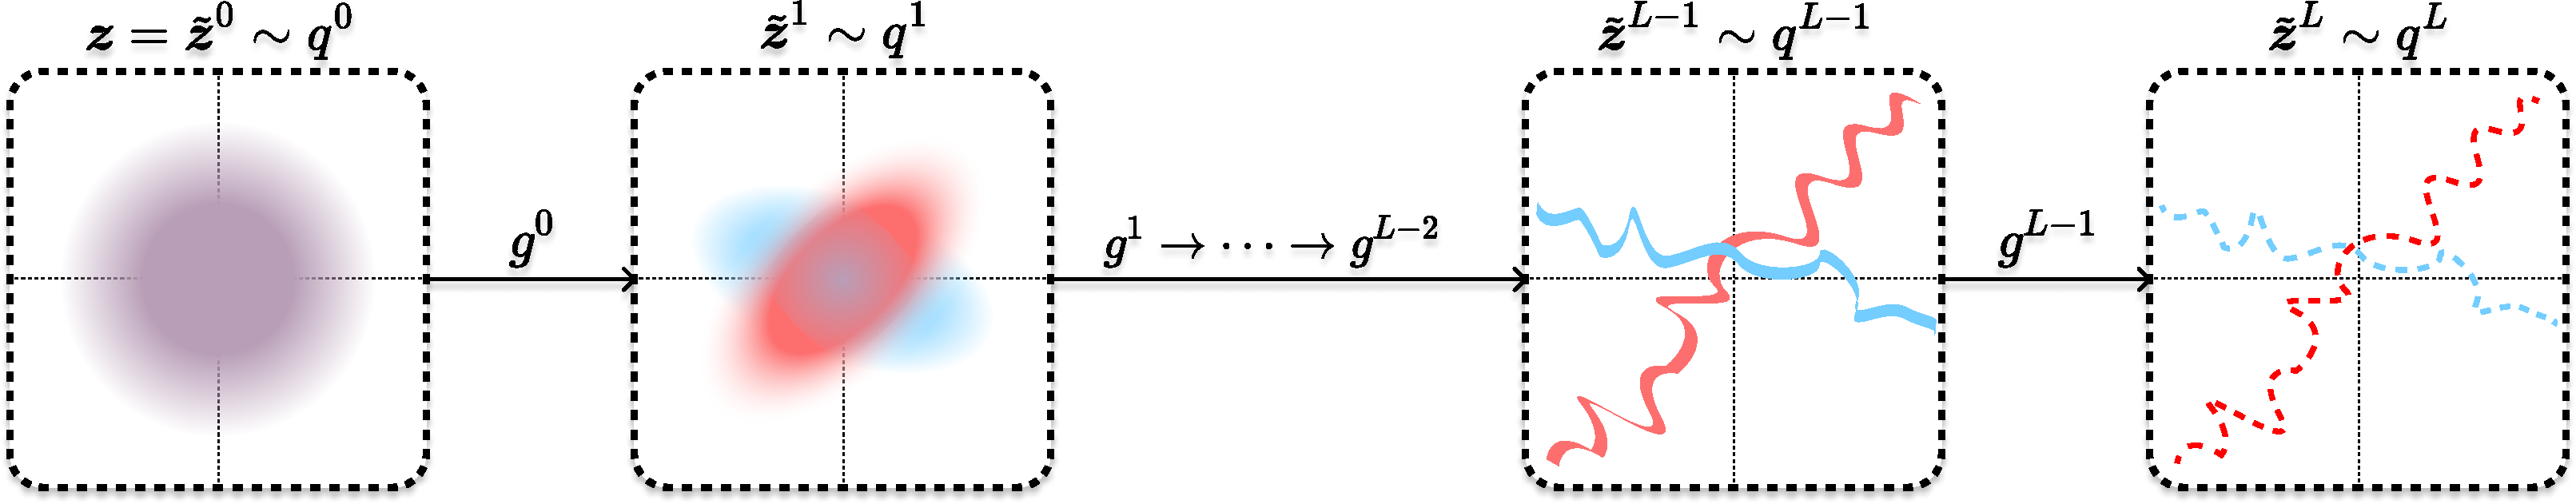
\includegraphics[width=\linewidth]{\toplevelprefix/chapters/chapter1/figs/diffusion_pipeline-2.pdf}
    \caption{Illustration of an iterative denoising and compressing process that, starting from a Gaussian distribution $q^0 = \mathcal{N}(\boldsymbol{0}, \boldsymbol{I})$, converges to an arbitrary low-dimensional data distribution $q^L = p(\x)$. }
    \label{fig:diffusion}
\end{figure}

Soon, denoising operators based on the score function \cite{hyvarinen05a}, briefly introduced in Section \ref{sec:denoising-intro}, were shown to be more general and unified the denoising and diffusion processes and algorithms \cite{song2019,song2020score,ho2020denoising}. Figure \ref{fig:diffusion} gives an illustration of the process that transforms a generic Gaussian distribution $q^0 = \mathcal{N}(\boldsymbol{0}, \boldsymbol{I})$ to an (arbitrary) empirical distribution $p(\x)$ by performing a sequence of iterative denoising (or compressing) operations:
\begin{equation}
        \z^0 \sim  \mathcal{N}(\boldsymbol{0}, \boldsymbol{I})\xrightarrow{\hspace{2mm} g^0  \hspace{2mm}} \z^1 \xrightarrow{\hspace{2mm} g^1 \hspace{2mm}} \cdots \xrightarrow{\hspace{2mm} g^{L-1}  \hspace{2mm}} \z^L \sim p(\x).
\end{equation}
By now, denoising (and diffusion) have replaced GANs and become a mainstream method for learning distributions of images and videos, leading to popular commercial image generating engines such as Midjourney and Stability.ai. 
In Chapter \ref{ch:compression} we will systematically introduce and study the denoising and diffusion method for learning a general low-dimensional distribution.  



\section{A Unifying Approach}\label{sec:unifying-approach}
So far, we have given a brief account of the main objective and history of machine intelligence and many important ideas and approaches associated with it. In recent years, after the empirical success of deep neural networks, tremendous efforts have been made to develop theoretical frameworks that can help us understand all the empirically designed deep neural networks, either certain seemingly necessary components (e.g., dropout,  normalization, attention, etc.) or their overall behaviors (e.g., double descent, neural collapse,  etc.). 

Partly motivated by this, this book aims to achieve several important and challenging goals: 
\begin{itemize}
    \item Develop a theoretical framework that would allow us to derive rigorous mathematical interpretation of deep neural networks.
    \item Ensure correctness of the learned data distribution and consistency with the learned representation.
    \item Demonstrate that the framework can lead to performant architectures and can guide further improvements in practice.
\end{itemize}
Within the past few years, there is mounting evidence that these goals can indeed be achieved, by leveraging the theory and solutions to the classical analytical low-dimensional models discussed briefly earlier (more thoroughly in Chapter \ref{ch:classic}) and by integrating fundamental ideas from a few related fields, namely information/coding theory, control/game theory, and optimization. This book aims to give a systematic introduction to this new approach.

\subsection{Learning Parsimonious Representations}
\label{sec:computational-approach-compression}
One necessary condition for any  learning task to be possible is that the sequences of interest must be {\em computable}, at least in the sense of Alan Turing \cite{Turing-1936}. That is, a sequence can be computed via a program on a typical computer.\footnote{There are indeed well-defined sequences that are not computable.} In addition to being computable, we require computation be {\em tractable}.\footnote{We do not need to consider predicting things whose computational complexity is intractable, say grows exponentially in the length or dimension of the sequence.} That is, the computational cost (space and time) for learning and computing the sequence should not grow exponentially in length. Furthermore, as we see in nature (and in modern practice of machine intelligence), for most practical tasks, an intelligent system needs to learn what is predictable from massive data in a very high-dimensional space, such as from vision, sound, and touch. Hence, for intelligence, we do not need to consider all computable and tractable sequences or structures. We should focus only on predictable sequences and structures which admit {\em scalable} realizations of its learning and computing algorithms:
\begin{equation}
\mbox{\textbf{computable}} \;
   \Longrightarrow \; \mbox{\textbf{tractable}} \; \Longrightarrow \; 
   \mbox{\textbf{scalable}}.
\end{equation}

This is because whatever algorithms intelligent beings use to learn useful information must be {\em scalable}. More specifically, the computational complexity of the algorithms would better scale gracefully, typically linear or even sublinear, in the size and dimension of the data. On the technical level, this requires that the operations that the algorithms rely on to learn could only utilize oracle information that can be efficiently computed from the data. More specifically, when the dimension is high and the scale is large, the only oracle one could afford to compute is either the first-order geometric information about the data\footnote{such as approximating a nonlinear structure locally with linear subspaces and computing the gradient of an objective function.} or the second-order statistic information\footnote{such as covariance or correlation of the data or their features.}.
The main goal of this book is to develop a theoretical and computational framework within which we can systematically develop efficient and effective solutions or algorithms with such scalable oracles and operations to {\em learn} low-dimensional structures from the sampled data and subsequently the predictive function.


\paragraph{Pursuing low-dimensionality via compression.}

2015年,在生成对抗网络(GAN)问世并广受欢迎后不久,Surya Ganguli及其学生意识到并提出,一个由深度网络建模的迭代去噪过程可用于学习通用分布,例如自然图像的分布 \cite{Sohl-Dickstein2015}。他们的方法受到了特殊高斯过程和二项过程性质的启发,这些性质由William Feller早在1949年就已研究 \cite{Feller1949OnTT}。\footnote{这又是在神奇的20世纪40年代!} 

\begin{figure}[t]
    \centering
    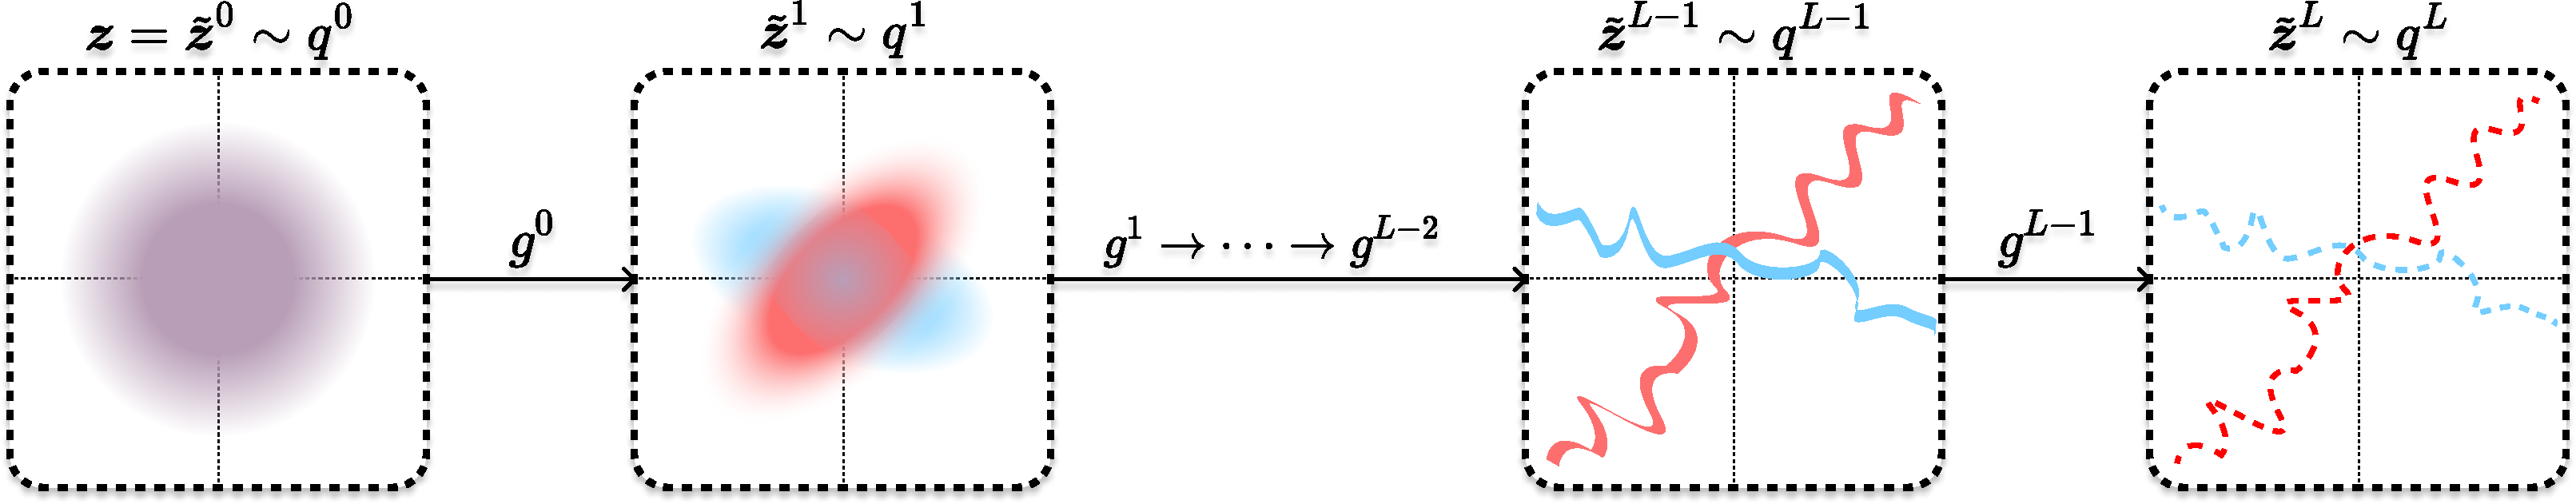
\includegraphics[width=\linewidth]{\toplevelprefix/chapters/chapter1/figs/diffusion_pipeline-2.pdf}
    \caption{一个迭代去噪与压缩过程的示意图,该过程从一个高斯分布 $q^0 = \mathcal{N}(\boldsymbol{0}, \boldsymbol{I})$ 出发,最终收敛至一个任意的低维数据分布 $q^L = p(\x)$。}
    \label{fig:diffusion}
\end{figure}

不久之后,基于分数函数 \cite{hyvarinen05a} 的去噪算子(在 \ref{sec:denoising-intro} 节中已简要介绍)被证明更具通用性,并统一了去噪与扩散的过程及算法 \cite{song2019,song2020score,ho2020denoising}。图 \ref{fig:diffusion} 展示了这一过程,它通过执行一系列迭代的去噪(或压缩)操作,将一个通用高斯分布 $q^0 = \mathcal{N}(\boldsymbol{0}, \boldsymbol{I})$ 转换为一个(任意的)经验分布 $p(\x)$:
\begin{equation}
        \z^0 \sim  \mathcal{N}(\boldsymbol{0}, \boldsymbol{I})\xrightarrow{\hspace{2mm} g^0  \hspace{2mm}} \z^1 \xrightarrow{\hspace{2mm} g^1 \hspace{2mm}} \cdots \xrightarrow{\hspace{2mm} g^{L-1}  \hspace{2mm}} \z^L \sim p(\x).
\end{equation}
如今,去噪(与扩散)模型已取代生成对抗网络,成为学习图像和视频分布的主流方法,并催生了如Midjourney和Stability.ai等广受欢迎的商业图像生成引擎。
在第 \ref{ch:compression} 章中,我们将系统地介绍和研究用于学习通用低维分布的去噪与扩散方法。  



\section{一个统一的框架}\label{sec:unifying-approach}
至此,我们已简要阐述了机器智能的主要目标与历史,以及与之相关的许多重要思想和方法。近年来,随着深度神经网络在经验上取得成功,学术界付出了巨大努力来发展理论框架,以帮助我们理解所有凭经验设计的深度神经网络,无论是某些看似必要的组件(例如,dropout、normalization、attention等),还是它们的整体行为(例如,double descent、neural collapse等)。

本书部分受此启发,旨在实现几个重要而富有挑战性的目标:
\begin{itemize}
    \item 发展一个理论框架,使我们能够推导出深度神经网络的严格数学解释。
    \item 确保所学数据分布的正确性,及其与所学表征的一致性。
    \item 证明该框架能够催生高性能的架构,并能指导实践中的进一步改进。
\end{itemize}
在过去几年中,越来越多的证据表明,这些目标确实可以实现。其途径是,利用我们先前简要讨论过(并将在第 \ref{ch:classic} 章中更深入探讨)的经典解析低维模型的理论与解法,并融合来自几个相关领域的基本思想,即信息/编码理论、控制/博弈论以及优化理论。本书旨在对这一新方法进行系统的介绍。

\subsection{学习简约表征}
\label{sec:computational-approach-compression}
任何学习任务得以实现的必要条件之一是,目标序列必须是{\em 可计算的}(computable),至少是在艾伦·图灵(Alan Turing)\cite{Turing-1936} 的意义上。也就是说,一个序列可以通过典型计算机上的程序来计算。\footnote{确实存在一些定义明确但不可计算的序列。} 除了可计算之外,我们还要求计算是{\em 易于处理的}(tractable)。\footnote{我们无需考虑预测那些计算复杂度难解的事物,例如其复杂度随序列长度或维度呈指数级增长。} 也就是说,学习和计算该序列的计算成本(空间和时间)不应随其长度呈指数级增长。此外,正如我们在自然界(以及在现代机器智能实践)中所见,对于大多数实际任务,智能系统需要从高维空间的海量数据(例如视觉、声音和触觉数据)中学习可预测的内容。因此,对于智能而言,我们无需考虑所有可计算和易于处理的序列或结构。我们应只关注那些其学习和计算算法拥有{\em 可扩展}(scalable)实现的、可预测的序列和结构:
\begin{equation}
\mbox{\textbf{可计算}} \;
   \Longrightarrow \; \mbox{\textbf{易处理}} \; \Longrightarrow \; 
   \mbox{\textbf{可扩展}}。
\end{equation}

这是因为智能体用于学习有用信息的任何算法都必须是{\em 可扩展的}。更具体地说,算法的计算复杂度最好能随着数据规模和维度的增加而良好地扩展,通常是线性甚至亚线性的。在技术层面上,这要求算法所依赖的学习操作只能利用那些能从数据中高效计算出的神谕信息。更具体地说,当维度很高、规模很大时,人们唯一能负担得起计算的神谕,要么是关于数据的一阶几何信息\footnote{例如用线性子空间局部逼近非线性结构,以及计算目标函数的梯度。},要么是二阶统计信息\footnote{例如数据或其特征的协方差或相关性。}。
本书的主要目标是发展一个理论和计算框架,在此框架内,我们可以利用这类可扩展的神谕和操作,系统地开发出高效且有效的解法或算法,以从采样数据中{\em 学习}低维结构,并进而学习预测函数。


\paragraph{通过压缩追求低维性。}

从我们在第 \ref{sec:predictability} 节中给出的序列示例可以清楚地看到,有些序列易于建模和计算,而另一些则较为困难。显然,一个序列的计算成本取决于其预测函数 $f$ 的复杂程度。回归阶数 $d$ 越高,计算成本就越大。$f$ 可以是一个简单的线性函数,也可以是一个其指定和计算可以任意复杂的非线性函数。

我们有理由相信,无论我们选择何种度量标准,如果一个序列更难以指定和计算,那么从其采样片段中学习也将更加困难。然而,对于任何给定的可预测序列,实际上存在多种(通常是无限多种)指定它的方法。例如,对于一个简单的序列 $x_{n+1} = a x_{n}$,我们也可以用 $x_{n+1} = a x_n + b x_{n-1} - b x_{n-1}$ 来定义同一个序列。
因此,如果我们能为任何给定的可计算序列发展出一种客观而严谨的“复杂性”概念,那将非常有益。

俄罗斯数学家安德雷·柯尔莫哥洛夫 (Andrey Kolmogorov) 是最早为任何可计算序列给出复杂性定义的人之一。\footnote{许多人都对序列复杂性这一概念做出了贡献,其中最著名的包括雷·所罗门诺夫 (Ray Solomonoff) 和格雷戈里·蔡廷 (Greg Chaitin)。人们普遍认为,这三位学者各自独立地发展和研究了算法信息论:雷·所罗门诺夫于 1960 年,安德雷·柯尔莫哥洛夫于 1965 年 \cite{Kolmogorov1998OnTO},以及格雷戈里·蔡廷于 1966 年左右 \cite{Chaitin-1966}。} 他提出,在所有能够计算同一序列的程序中,我们可以用最短程序的长度来度量其复杂性。这个想法与著名的“奥卡姆剃刀”简约性原则非常一致:{\em 在所有能够解释相同观察结果的理论中,我们总是选择最简单的那一个。} 更确切地说,设 $p$ 表示一个可以在通用计算机 $\mathcal{U}$ 上生成序列 $S$ 的计算程序。序列 $S$ 的柯尔莫哥洛夫复杂性定义为:
\begin{equation}
    K(S) = \min_{p\,:\, \mathcal{U}(p) = S} L(p). 
\end{equation}
因此,一个序列的复杂性是由我们能以多么“简约”的方式来指定或计算它来衡量的。这种关于序列复杂性(或简约性)的定义具有重要的概念意义,并拥有许多有趣的性质。在历史上,它启发了计算理论领域的许多深刻研究,尤其是在算法信息论领域。

最短程序的长度可以被看作是所考虑序列的终极压缩,它提供了一个定量的度量,衡量我们通过学习序列的正确生成机制获得了多大的收益。然而,尽管具有重要的理论意义,柯尔莫哥洛夫复杂性通常不是一个可计算函数 \cite{Cover-Thomas}(甚至难以精确近似)。因此,这种复杂性度量几乎没有实际用途。它既不能预先告诉我们学习一个给定序列的难度,也不能告诉我们学得有多好。





% 简约性或紧凑性的度量:度量数据紧凑性的多种(很大程度上等价的)方法:柯尔莫哥洛夫复杂性(不可计算)、数据分布(支撑集)的维度和体积、最小描述长度、率失真等。

\paragraph{简约性的可计算度量。}

因此,出于实践目的,我们需要一种可有效计算的复杂度度量,用以衡量由同一预测函数生成的序列。\footnote{注意,在实践中,我们通常关心的是学习预测函数 $f$ 本身,而非由 $f$ 生成的任何特定序列。} 值得注意的是,柯尔莫哥洛夫复杂度之所以不可计算,部分原因在于其定义是非构造性的。

因此,为了引入一种可计算的复杂度度量,我们可以采纳一种更具构造性的方法,正如克劳德·香农在信息论框架 \cite{Shannon-1948,Cover-Thomas} 中所倡导的那样。\footnote{在过去80多年里,该理论成功地指导了通信行业的工程实践。} 本质上,通过假设序列 $S$ 是从一个概率分布 $p(S)$ 中抽取的,该分布的所谓{\em 熵} (entropy):\footnote{此处我们考虑的是微分熵,因为我们假设序列由连续变量组成。如果序列由离散变量组成,我们则可以考虑(离散)熵:$H(S) = - \sum_{i}p(s_i) \log p(s_i).$}
\begin{equation}
    h(S) \doteq -\int p(s) \log p(s) \odif{s}
    \label{eqn:entropy-definition}
\end{equation}
给出了其复杂度的一种自然度量。这种度量也有一种自然的解释,即编码这样一个序列所需的平均二进制比特数,这一点我们将在第 \ref{ch:compression} 章中看到。

为了阐释这一观点的主要思想,我们考虑大量由预测函数 $f$ 生成的长序列片段:
\begin{equation}
    \{S_1, S_2, \ldots, S_i, \ldots, S_N\} \subset \mathbb{R}^D,
\end{equation}
注意,不失一般性地,此处我们假设所有序列的长度均为 $D$。因此,每个序列都可以被看作是 $\mathbb{R}^D$ 空间中的一个向量。其次,我们可以引入一种记作 $\mathcal E$ 的编码方案(包含一个码本),它将每个片段 $S_i$ 转换为一个唯一的二进制比特流 $\mathcal{E}(S_i)$。最简单的编码方案是用 $\epsilon$-球来填充所有片段所张成的空间,如图 \ref{fig:coding-schemes} 所示。然后我们对所有的球进行编号。每个序列被编码为其最近的球的(二进制)编号。因此,每个片段都可以从其对应的比特流中恢复\footnote{因为这是一种有损编码方案,所以恢复的精度在 $\epsilon$ 之内。}出来。
\begin{figure}
    \centering
    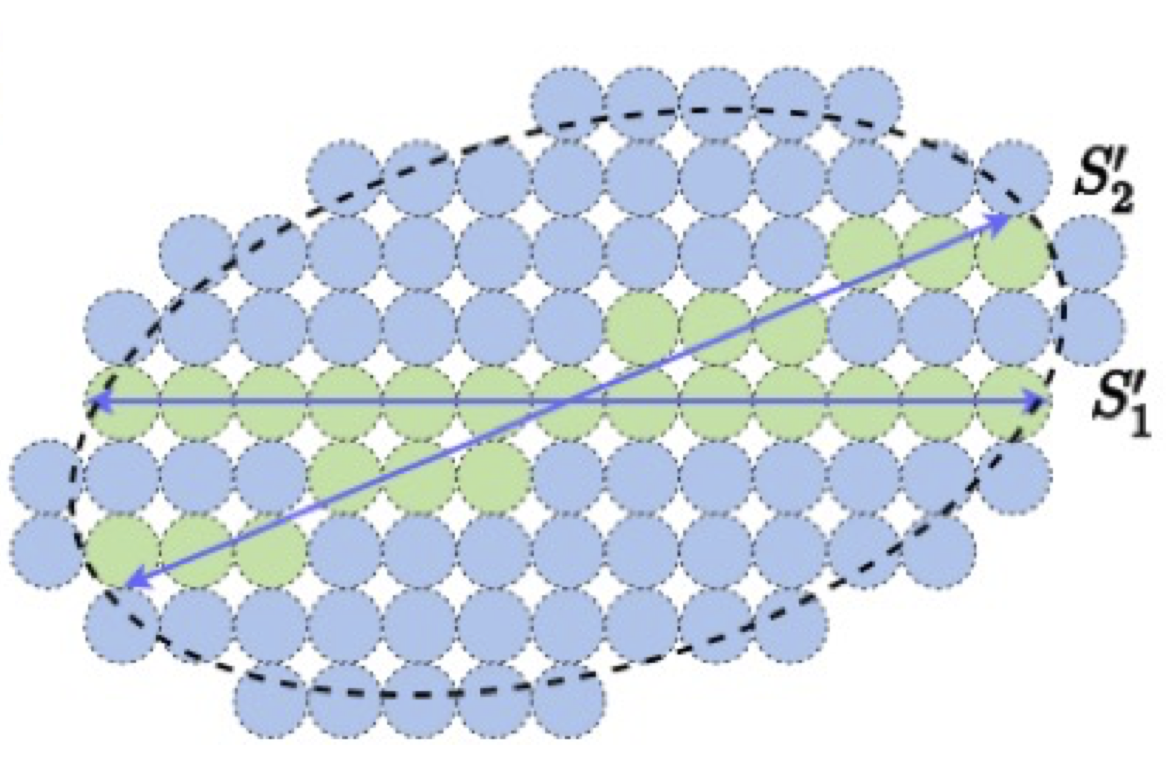
\includegraphics[width=0.5\linewidth]{\toplevelprefix/chapters/chapter1/figs/Coding-schemes.png}
    \caption{两种编码方案的比较。假设数据的真实分布位于两条箭头线周围。我们可以用包含所有蓝球的码本来编码来自这两条线上的样本;也可以用只包含绿球的码本来编码这些样本。显然,在相同精度下,第二种编码方案将得到更短的编码长度/更低的编码率。}
    \label{fig:coding-schemes}
\end{figure}

于是,预测函数 $f$ 的复杂度可以通过所有序列的平均编码长度来评估,这被称为编码率:\footnote{更精确地说,我们可以将 $R(f\mid \mathcal{E})$ 定义为所有长度为 $D$ 的片段的期望编码长度。}
\begin{equation}
   R(f \mid \mathcal E) = \mathbb{E}[L(\mathcal{E}(S))] \approx \frac{1}{N}\sum_{i=1}^N L(\mathcal{E}(S_i)). 
   \label{eqn:coding-rate}
\end{equation}
显然,如果使用不同的编码方案(或码本),编码率这一度量也会随之改变。在实践中,我们对数据片段所围绕分布的低维结构了解得越透彻,就能设计出越高效的码本,如图 \ref{fig:coding-schemes} 所示。敏锐的读者可能已经意识到,从概念上讲,图 \ref{fig:diffusion} 中所示的去噪过程,与从采用蓝色球的编码方案转变为采用绿色球的方案非常相似。


给定两种针对数据片段的编码方案 $\mathcal{E}_1$ 和 $\mathcal{E}_2$,如果二者的编码率之差为正:
\begin{equation}
   R(f \mid \mathcal E_1) -  R(f \mid \mathcal E_2) > 0, 
\end{equation}
我们便可以说编码方案 $\mathcal{E}_2$ 更优。这个差值可以看作一个度量,它衡量了关于数据分布,编码方案 $\mathcal{E}_2$ 相较于 $\mathcal{E}_1$ 多掌握了多少信息。在很大程度上,学习 $f$ 的目标等价于找到能最小化编码率的最优编码方案:
\begin{equation}
   \min_{\mathcal{E}} R(f \mid \mathcal E). 
\end{equation}
正如我们将在第 \ref{ch:compression} 章中看到的,可达到的最小编码率与熵 $H(S)$(见公式 \eqref{eqn:entropy-definition})的概念密切相关。


\begin{remark}\label{rem:computable-complexity}
    {用显式编码方案度量数据复杂度的视角,催生了若干旨在修正柯尔莫哥洛夫复杂度以提升其可计算性的学习目标 \cite{WallaceC1999},其中包括 1968 年提出的最小消息长度(MML)\cite{WallaceC1968} 和 1978 年提出的最小描述长度(MDL)\cite{Rissanen-1978,HansenM2001}。这些目标除了计算目标数据 $S$ 的编码长度外,通常还计算编码方案 $\mathcal{E}$ 本身(包括其码本)的编码长度:$L(\mathcal E(S)) + L(\mathcal E)$。然而,如果目标是学习一个有限大小的码本并将其应用于大量序列,那么码本的摊销成本可以忽略不计,因为当 $N$ 变得很大时,$$\frac{1}{N}\Big( L(\mathcal{E}) + \sum_{i=1}^N L(\mathcal{E}(S_i))\Big) \approx \frac{1}{N}\sum_{i=1}^N L(\mathcal{E}(S_i))$$。}
\end{remark}

再次强调,我们可以将最终得到的最优编码方案,视为对观测数据实现了最佳压缩的方案。一般而言,与柯尔莫哥洛夫复杂度相比,任何特定编码方案所给出的编码长度总是更大的:
\begin{equation}
    K(S) < L( \mathcal E(S)).
\end{equation} 
因此,最小化编码率/编码长度,本质上是在最小化那个不可计算的柯尔莫哥洛夫复杂度的一个上界。

\subsection{学习信息丰富的表示}

%\paragraph{通过信息增益实现结构化表示。}
请注意,如果目标仅仅是为压缩而压缩,那么理论上,逼近柯尔莫哥洛夫复杂度的最优编码将变得近乎随机或无结构 \cite{Chaitin-1966}。\footnote{因为任何有结构的代码都可以被进一步压缩。}然而,我们学习预测函数 $f$ 的真正目的,是在未来的预测中能够方便地反复使用它。因此,尽管压缩能帮助我们识别数据中的低维分布,我们仍希望以一种{\em 结构化、有组织}的方式对该分布进行编码,从而使得最终得到的表示信息量丰富且易于使用。\footnote{例如,在不同条件下对该分布进行采样。}图 \ref{fig:expansion} 通过一个例子直观地解释了为何需要这样的变换。

\begin{figure}
    \centering
    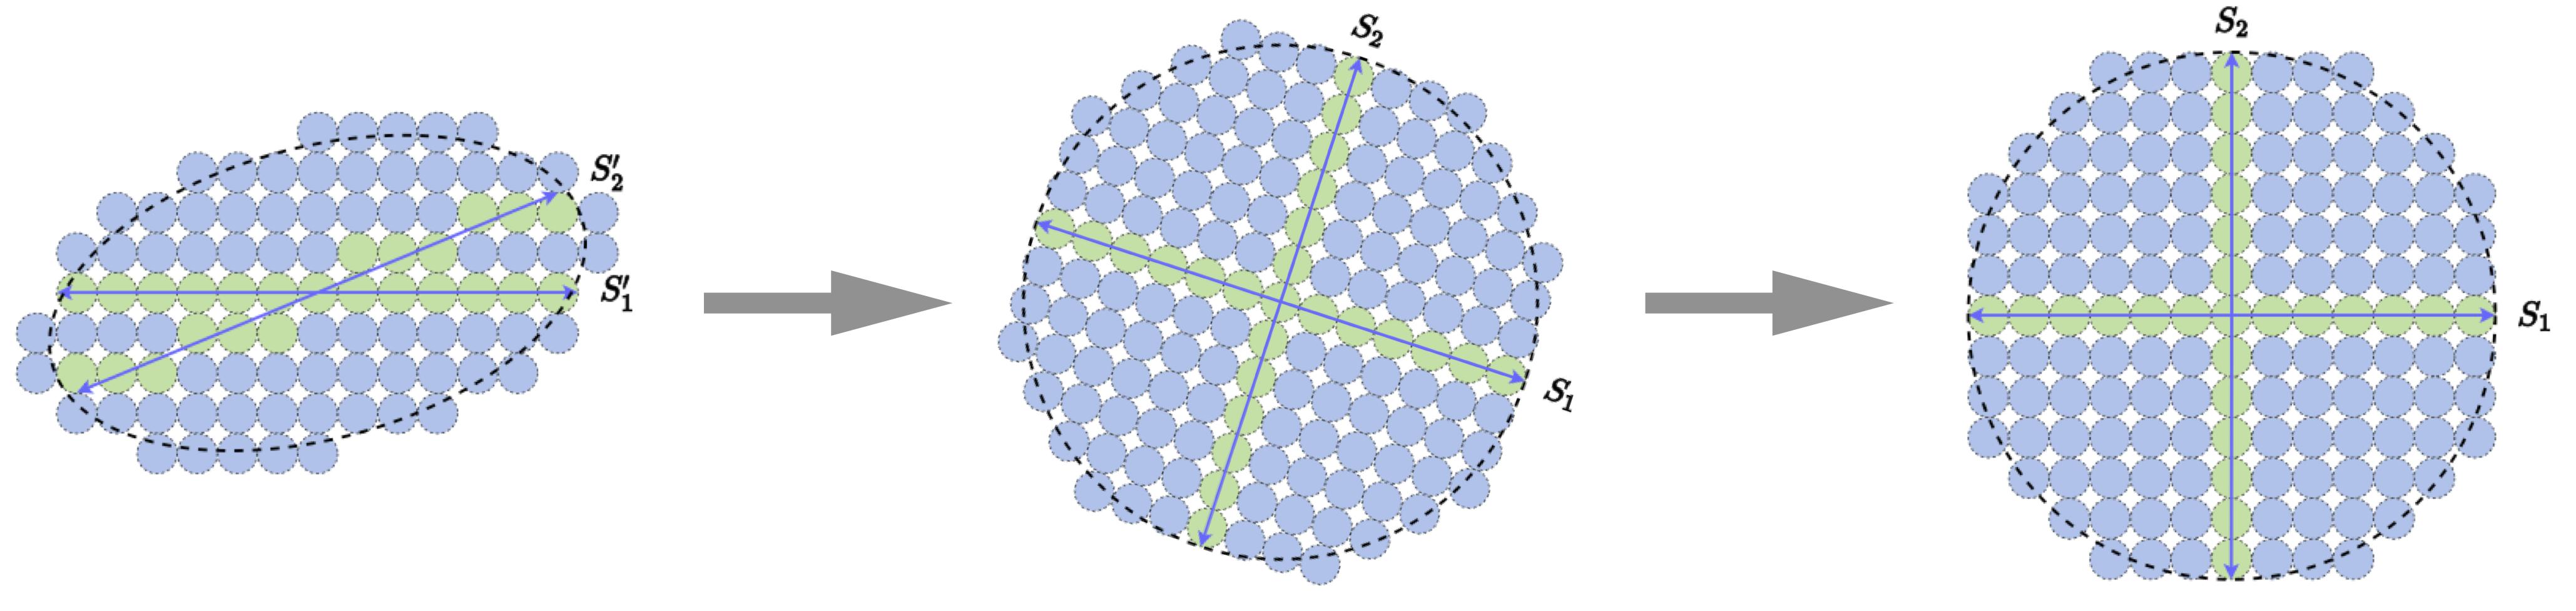
\includegraphics[width=0.98\linewidth]{\toplevelprefix/chapters/chapter1/figs/coding-transform.png}
    \caption{将已识别的低维数据分布变换为信息更丰富、结构更清晰的表示。}
    \label{fig:expansion}
\end{figure}
正如我们将在第 \ref{ch:compression} 章中展示的,通过选择一种基于所选编码方案之编码率的自然度量——即{\em 信息增益},可以精确地促进最终表示中这些理想结构的形成。正如我们在本书中将反复看到的,这种显式且构造性的编码方法,为学习真实世界数据中低维结构的良好表示提供了一个强大的计算框架。因为在许多具有重要实用价值的情况下,编码长度函数可以被高效地计算或精确地近似。在一些理想情况下,我们甚至可以获得解析解,例如子空间和高斯分布(见第 \ref{ch:compression} 章)。

此外,这样的计算框架引出了一种原则性的方法,它自然地揭示了深度网络在这一学习过程中所扮演的角色。正如我们将在第 \ref{ch:representation} 章中系统地推导的,深度网络的每一层都在试图以增量的方式执行优化目标函数的操作。从这个角度来看,深度网络的作用可以被精确地解释为模拟某个迭代优化算法(例如梯度下降法),以优化信息增益这一目标。由此产生的深度网络架构的每一层都可以被赋予精确的统计和几何解释,即执行增量的压缩编码和解码操作。最终,我们推导出的深度网络将成为透明的“白盒”,在数学上是完全可以解释的。



% \textbf{注记:} 将可预测性转化为低维性:这类数据的一个普遍数学特性是,在其所嵌入的通常是高维的空间中,它们的分布总是具有非常低的内在维度,因此是高度可压缩的。

% %促进低维性的其他相关性,例如许多由偏微分方程描述的物理定律,如电磁场的麦克斯韦方程组和流体动力学的纳维-斯托克斯方程。

% 紧凑性的度量:度量数据紧凑性的多种(在很大程度上等价的)方法:柯尔莫哥洛夫复杂度(不可计算)、数据分布(支撑集)的维度和体积、最小描述长度、率失真等。

% 因此,学习源于可预测性的低维结构的一种有效方法,是通过旨在最小化此类度量的某种“压缩”操作(我们稍后将给出精确定义)。





\subsection{学习一致的表示}

%\subsection{确保一致性}
\label{sec:consistency}
总结我们到目前的讨论,我们将数据表示为:
\begin{equation}
    \boldsymbol{X} = \{S_1, S_2, \ldots, S_i, \ldots, S_N\} \subset \mathbb{R}^D,
\end{equation}
并令 $\boldsymbol{Z} = \mathcal{E}(\X)$ 为通过某个编码器 $\mathcal{E}$ 得到的 $\X$ 的编码:
\begin{equation}
    \X  \xrightarrow{\hspace{2mm} \mathcal{E}\hspace{2mm}} \Z.
    \label{eqn:open-loop}
\end{equation}

在机器学习的语境中,$\Z$ 通常被称为“特征” (features) 或“潜在表示” (latent representation)。值得注意的是,若不知道 $\X$ 的底层分布,我们将无从知晓何种编码器 $\mathcal{E}$ 能够保留关于 $\X$ 分布的最多有用信息。在实践中,人们通常会先尝试某种适用于特定任务的紧凑编码方案。具体而言,他们会试图学习一个能优化所学表示的某种(经验性)简约性度量 (measure of parsimony) 的编码器:
\begin{equation}
    \min \rho(\Z). 
\end{equation}

\begin{example}
例如,图像分类便是如此:我们将同一类别中的所有图像赋予同一个编码,而不同类别中的图像则赋予不同的编码,比如“独热” (one-hot) 向量:
\begin{equation}
  \x \mapsto \z \in \{  [1, 0, 0, \ldots , 0, 0], \;  [0, 1, 0 \ldots, 0, 0], \; \ldots, \;  [0,0,0, \ldots, 0, 1].\}
  \label{eqn:class-labels}
\end{equation}
现在,一个分类器 $f(\cdot)$ 可以被建模为一个函数,用以预测给定的 $\x$ 属于 $K$ 个类别中每一个的概率:$\hat{\z} = f(\x) \in \mathbb{R}^K$。于是,分类器的“优劣” (goodness) 可以通过所谓的{\em 交叉熵} (cross entropy) 来衡量:\footnote{交叉熵可以被看作是 $\z$ 的真实分布与预测 $\hat\z$ 的分布之间的一种距离度量。它也可以被看作是 $\z$ 的期望编码长度——如果我们使用针对 $\hat\z$ 的最优码本来对 $\z$ 进行编码。当 $\z$ 和 $\hat\z$ 具有相同分布时,交叉熵达到最小值。}
\begin{equation}
    L(\hat{\z}, \z) = \sum_{k=1}^K - z_k \log \hat{z}_k,
\end{equation}
其中 $z_k$ 表示向量 $\z$ 的第 $k$ 个分量。正如深度网络的早期实践 \cite{krizhevsky2012imagenet} 所表明的,如果给予足够的数据,这种编码方案通常可以由一个深度网络来表示,并通过优化交叉熵以端到端 (end-to-end) 的方式学习得到。
\end{example}

交叉熵损失 $L(\hat \z, \z)$ 可被视为一种特殊的简约性度量 $\rho(\z)$,它与一类适用于分类的特定编码方案族相关联。然而,这种编码显然是{\em 极具损失性的} (very lossy)。所学得的 $\Z$ 除了其类别类型外,不包含关于 $\X$ 的任何其他信息。例如,通过为一个图像赋予(代表)类别标签“苹果”的编码,我们仅从该标签本身,已无法得知原始图像中苹果的具体种类。

当然,另一个极端是要求编码方案是{\em 无损的} (lossless)。也就是说,在 $\x$ 和其编码 $\z$ 之间存在一一映射。然而,正如我们将在第 \ref{ch:compression} 章中看到的,除非 $\x$ 是离散的,否则无损编码(或压缩)是不切实际的。对于一个连续随机变量,我们可能只考虑有损编码方案,从而使数据的编码长度有限。也就是说,我们仅以某个预设的精度对数据进行编码。正如我们将在第 \ref{ch:compression} 章中进一步阐述的,有损编码不仅仅是一个现实的选择,它在“使得从分布的有限样本中学习其底层连续分布成为可能”这一过程中,扮演着至关重要的角色。

出于许多学习目的,我们希望特征 $\z$ 即便是{\em 有损的},也能保留比其类别类型更多的关于 $\x$ 的信息。在本书中,我们将介绍一种更具普适性的简约性度量,该度量基于编码长度/率,并与一个更通用的编码方案族——即用子空间混合或高斯混合进行编码——相关联。该方案族能够以特定精度紧密地近似任意真实世界的分布。正如我们将在第 \ref{ch:compression} 章和第 \ref{ch:representation} 章中看到的,这样一种度量不仅会保留关于 $\X$ 分布的绝大部分信息,还将为所学得的表示 $\Z$ 促成某些理想的、优良的几何和统计结构。


\paragraph{为实现一致性的双向自动编码 (Bidirectional Autoencoding for Consistency)。}
在更广泛的学习语境中,压缩编码方案 $\mathcal{E}$ 的主要目标是识别数据 $\X$ 中的低维结构,从而可以利用这些结构对原始数据空间进行预测。这要求所学得的编码方案 $\mathcal{E}$ 能够匹配一个高效的解码方案,记作 $\mathcal{D}$。该解码方案将通常称为隐表示的 $\Z$ 映射回原始数据空间:
\begin{equation}
    \X   \xrightarrow{\hspace{2mm} \mathcal{E}\hspace{2mm}} \Z  \xrightarrow{\hspace{2mm} \mathcal{D} \hspace{2mm}} \hat \X.
       \label{eqn:auto-encoding}
\end{equation}
通常,我们将这样的编码和解码对 $(\mathcal{E}, \mathcal{D})$ 称为{\em 自编码} (autoencoding)。图 \ref{fig:autoencoder}
展示了这样一个自编码器的过程。
\begin{figure}
    \centering
    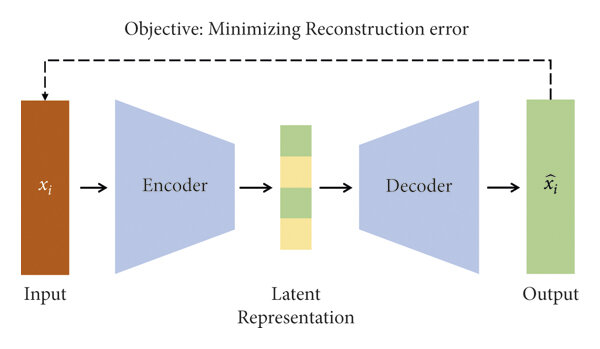
\includegraphics[width=0.7\linewidth]{\toplevelprefix/chapters/chapter1/figs/Autoencoder.jpg}
    \caption{自编码器架构示意图。}
    \label{fig:autoencoder}
\end{figure}


通常,我们希望解码过程近似于编码的“逆”过程,使得从 $\Z$ 解码出的数据(分布)$\hat \X$ 能在一定程度上与原始数据(分布)$\X$ 相似。\footnote{我们稍后将更精确地阐述“相似”的含义。}如果能做到这一点,我们便能够从 $\Z$ 中恢复或预测原始数据空间中的信息。在这种情况下,我们称 $(\mathcal{E}, \mathcal{D})$ 对构成了一个{\em 一致的} (consistent) 自编码。对于大多数实际应用而言,我们不仅需要这样的解码方案存在,还需要它能够被高效地实现和物理地部署。例如,如果 $\x$ 是一个实值变量,则需要进行量化,才能使任何解码方案都可以在有限状态机上实现,正如我们将在第 \ref{ch:compression} 章中详细解释的那样。因此,通常来说,我们应当预见到,可实现的编码和解码方案必然是有损的。一个核心问题是,如何学习一个紧凑的(有损的)表示 $\Z$,使其能很好地用于预测 $\X$。

一般而言,正如我们将看到的,编码器和解码器都可以通过深度网络来建模和实现,并通过求解如下形式的优化问题来学习:
\begin{equation}
   \min \, d( \X, \hat \X) + \rho(\Z), 
   \label{eqn:auto-encoding-objective}
\end{equation}
其中 $d(\cdot, \cdot)$ 是一个特定的距离函数,旨在促进 $\X$ 和 $\hat \X$ 之间的相似性\footnote{相似性可以是样本层面上的,也可以是分布层面上的,具体取决于距离函数 $d$ 的选择。},而 $\rho(\Z)$ 是某个度量,旨在促进 $\Z$ 的简约性和信息丰富性。经典的主成分分析 (PCA) \cite{JolliffeI2002} 是一致性自编码的一个典型例子,我们将在第 \ref{ch:classic} 章中对此进行深入研究,并将其作为通向更一般的低维结构的先导。在第 \ref{ch:autoencoding} 章中,我们将研究如何学习一致性自编码,以处理一般的(例如非线性的)低维分布。


\subsection{学习自洽表示}
请注意,在上述自编码目标中,需要评估解码数据 $\hat \X$ 与原始数据 $\X$ 的接近或一致程度。这通常需要外部的监督或关于使用何种相似性度量的知识。计算 $\hat \X$ 与 $\X$ 之间的相似性可能代价高昂,甚至完全不可能或难以处理。\footnote{例如,假设我们想要最小化两者之间的某种分布距离。} 值得注意的是,在自然界中,动物能够完全自主学习,而无需在数据空间中将其估计 $\hat \X$ 与基准真相 $\X$ 进行比较。它们通常甚至没有这样的选项。

那么,一个系统如何在没有外部监督或比较的情况下自主学习呢?它如何在不直接比较的情况下,便知晓 $\hat \X$ 与 $\X$ 是一致的呢?这引出了“闭环”的思想。事实证明,在我们将在第 \ref{ch:closed-loop} 章中详细阐述的温和条件下,为确保 $\X$ 和 $\hat \X$ 的一致性,只需将 $\hat \X$ 编码为 $\hat \Z$,并检验 $\Z$ 和 $\hat \Z$ 是否一致即可。我们将此一致性概念称为{\em 自洽性}(self-consistency),它可以通过以下图示来说明:
\begin{equation}
    \X   \xrightarrow{\hspace{2mm} \mathcal{E}\hspace{2mm}} \Z  \xrightarrow{\hspace{2mm} \mathcal{D} \hspace{2mm}} \hat \X \xrightarrow{\hspace{2mm} \mathcal{E}\hspace{2mm}} \hat \Z,
    \label{eqn:closed-loop}
\end{equation}
我们将此过程称为{\em 闭环转录}(closed-loop transcription),\footnote{其灵感来源于生物学中DNA与RNA或其他蛋白质之间的转录过程。} 如图 \ref{fig:closed-loop} 所示。

\begin{figure}[t]
    \centering
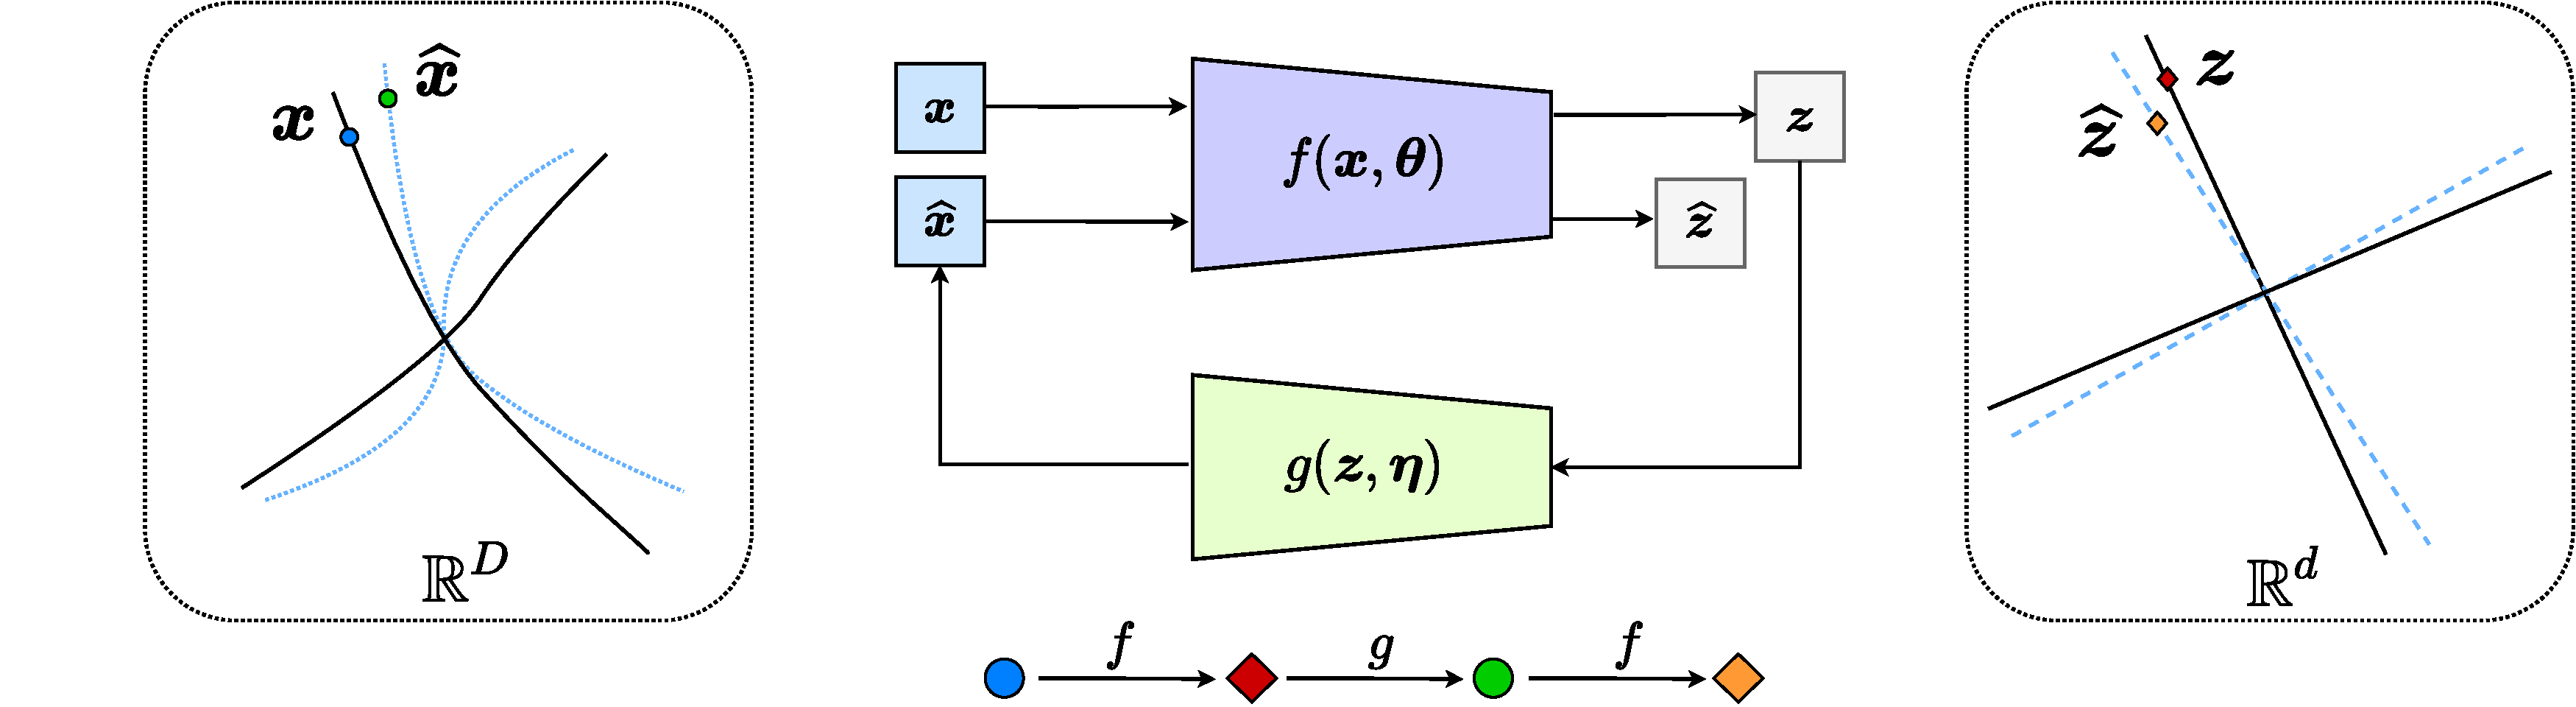
\includegraphics[width=0.9\linewidth]{\toplevelprefix/chapters/chapter1/figs/diagrams_redu_gan_2.pdf}
\caption{闭环转录示意图。此处我们用映射 $f$ 表示编码器 $\mathcal{E}$,用映射 $g$ 表示解码器 $\mathcal{D}$。}  \label{fig:closed-loop}
\end{figure}

可以说,任何自主智能体都只需学习观测数据 $\X$ 的一个自洽表示 $\Z$,因为在原始数据空间(通常指外部世界)中检验一致性,其代价不是过于高昂,就是物理上不可行。闭环范式允许我们通过一个仅依赖于内部(学习到的)特征 $\Z$ 的最小最大博弈,来学习一个最优的编码 $f(\cdot, \theta)$ 和解码 $g(\cdot, \eta)$:
\begin{equation}
\max_{\theta}\min_{\eta} \ell( \Z, \hat \Z) + \rho(\Z), 
   \label{eqn:closed-loop-objective}
\end{equation}
其中 $\ell( \Z, \hat \Z)$ 是一个基于特征 $\Z$ 和 $\hat \Z$ 编码率的损失函数,我们将看到,它的计算要容易得多。此处,$\rho(\Z)$ 同样是某种旨在提升 $\Z$ 的简约性和信息丰富度的度量。有些出人意料的是,我们将在第 \ref{ch:closed-loop} 章中看到,在相当温和的条件下(例如 $\X$ 的维度足够低),$(\Z, \hat \Z)$ 之间的自洽性竟然蕴含了 $(\X, \hat \X)$ 的一致性!此外,我们还将看到,闭环系统能让我们以一种{\em 连续和增量}的方式学习数据分布,\footnote{即一次学习一个类别,甚至一次学习一个样本。} 而不会遭受开环模型中常见的灾难性遗忘等问题。

\section{连接机器智能的理论与实践}
    
至此,我们已经介绍了三种相关的框架,用于为给定的数据分布 $\X$ 学习一个紧凑且结构化的表示 $\Z$:
\begin{itemize}
\item 开放式编码 \eqref{eqn:open-loop};
\item 双向自编码 \eqref{eqn:auto-encoding};
\item 闭环转录 \eqref{eqn:closed-loop}。
\end{itemize}
在本书中,我们将逐一系统地研究这三个框架:
\begin{equation}
    \mbox{\textbf{开放式}} \; \Longrightarrow \; 
    \mbox{\textbf{双向}} \;  \Longrightarrow \; \mbox{\textbf{闭环}},
\end{equation}
这三个框架将分别在第\ref{ch:representation}章、第\ref{ch:autoencoding}章的第\ref{sec:consistent-representation}节和第\ref{sec:self-consistency}节中进行探讨。

在过去几年中,学术界提出并发展了许多理论框架,以帮助理解深度网络。然而,许多框架未能提供可扩展的解决方案,使其在真实世界的数据和任务上的性能,媲美于经验方法。许多理论也未能为如何进一步改进实践提供有用的指导。第\ref{ch:conditional-inference}章和第\ref{ch:applications}章将展示本书提出的框架,如何帮助弥合理论与实践之间的鸿沟。第\ref{ch:conditional-inference}章将展示如何利用学习到的分布及其表示,来为那些依赖于条件估计和预测的实际任务,进行贝叶斯推断。第\ref{ch:applications}章将提供有力的实验证据,表明从第一性原理设计的网络和系统,可以在视觉表示学习、图像分类、图像补全、图像分割和文本生成等多种任务上,取得具有竞争力乃至更优的性能。


\paragraph{再论智能。}
如我们在开篇所提及的,任何智能体的一项基本任务,是从其感知的数据中学习可预测的信息。现在我们对这项任务的计算本质有了初步的了解,并且应当认识到,这是一个永无止境的过程,其原因如下:
\begin{itemize}
    \item 迄今为止从数据中学习到的知识(例如,通过编码和解码方案学得的知识),不大可能是完全正确或最优的。当预测新观测中仍存在误差时,智能应具备自我改进的能力。
    \item 迄今观测到的数据尚未涵盖所有可预测的信息。智能应能认识到当前知识的不足,并有能力在信息可得时随时学习和获取新知。
\end{itemize}

因此,智能并非是简单地预先收集所有数据,然后训练一个模型来记住数据中所有可预测的信息。恰恰相反,它关乎具备一种计算机制,该机制能在信息可得且有需要时,不断改进现有知识并获取新信息。也就是说,任何智能体或系统\footnote{例如一个动物、一个人类、一个智能机器人、整个科学界,乃至整个人类文明。}的一个基本特征是:{\em 能够自我持续地改进或获取信息(或知识)}。在概念上,我们可以用符号象征性地表示智能与信息(或知识)之间的关系如下:
\begin{equation}
\operatorname{智能}(t) = \odv*{\operatorname{信息}}{t}(t), \qquad 
\operatorname{信息}(t)  = \int_0^t \operatorname{智能}(s) \odif{s}.
\end{equation}
我们相信,闭环框架是一种普适的机制,它通过反馈\footnote{强化可以被看作是一种原始形式的反馈,例如来自大自然的自然选择。}或博弈\footnote{科学探究则可被视为一种最高级的博弈,它通过提出假设和验证假设来进行。}来实现自我改进和自我学习。自然界中所有的智能体或系统,在所有层面和所有尺度上,都利用闭环机制进行学习。这种机制的普遍性启发了早期的研究,这些研究试图用机器和计算机来建模与模拟智能,其中尤以诺伯特·维纳在20世纪40年代发起的控制论运动为著。

我们希望本书能帮助人们更好地理解智能背后的目标、原理和计算机制。它为未来进一步研究更高层次的人类智能——即真正的“人工智能”——奠定了基础。在本书的最后一章,即第\ref{ch:future}章中,我们将针对这些新方向,提出若干重大的开放性问题。

\end{document}

